\chapter{重述广义相对论——导数与曲率}

本章我们会引入导数,曲率以及它们的性质的旋量描述。重要的是,广义相对论作为一种“几何”理论,在旋量形式的重述下会变得更加简单和合理。


\section{流形}

我们已经有了流形上某一点旋量场的描述,那么如何描述时空流形上的点和其邻域,以及他们的切空间之间的关系?首先,如果要给出流形的切向量,其方向导数无疑是对流形上的标量场求导(记得$\boldsymbol{L} =\eta ^{-2} \partial /\partial \zeta +\overline{\eta }^{-2} \partial /\partial \overline{\zeta }$),那么实际上其方向导数描述的是标量场的“变化率”,即方向导数的性质完全由流形上的标量场的信息刻画。实际上,流形上的坐标系统也可以被看成一个标量场——因此,随后我们的尝试就是以标量场的形式来“定义”流形的结构。本节我们考虑的是实的$\mathbb{C}^{\infty }$标量场,由$\mathfrak{T}$表示,复的标量场$\mathfrak{S}$自然可以写为$\mathfrak{T} \oplus \mathrm{i}\mathfrak{T}$。同时目前为止我们考虑的都是$n$维的(豪斯多夫,仿紧,连通的)流形,直到后面才将其和时空等同起来。



那么考虑一个抽象的点集$\mathcal{M}$,上面的结构由$\mathfrak{T}$定义,每一个元素$f\in \mathfrak{T}$(即标量)是一个映射
\begin{equation*}
	f:\mathcal{M}\rightarrow \mathbb{R} .
\end{equation*}
如果我们给了$\mathfrak{T}$足够多的限制(后面称之为公理(axiom)),那么$\mathcal{M}$会成为一个可微流形,其微分结构就是$\mathfrak{T}$中的每个元素,即一个$\mathbb{C}^{\infty }$标量场。注意,这里我们给将要出的流形的定义和正常教科书中流形的定义完全等同。

\begin{post}[label={postulate 5.1}]{}
	如果$f_{1} ,f_{2} \cdots f_{r} \in \mathfrak{T}$,同时$F:\mathbb{R}^{r}\rightarrow \mathbb{R}$是一个任意的$r$个变量的$\mathbb{C}^{\infty }$实函数,那么$F( f_{1} ,f_{2} ,\cdots ,f_{r})$也是$\mathfrak{T}$中的一个元素。即
	\begin{equation*}
		F( f_{1} ,\cdots ,f_{r})( P) =F( f_{1}( P) ,\cdots ,f_{r}( P)) ,P\in \mathcal{M} .
	\end{equation*}
\end{post}

例如加法和乘法都是$\mathbb{C}^{\infty }$的映射$\mathbb{R}^{2}\rightarrow \mathbb{R}^{2}$,我们很自然给出
\begin{equation*}
	\begin{aligned}
		( f+g)( P) & \equiv f( P) +g( P) ,\\
		( fg)( P) & \equiv f( P) +g( P) .
	\end{aligned}
\end{equation*}
随后我们就要涉及到邻域的概念。我们称$P$的$\mathfrak{T}$-邻域是指对于某些$f\in \mathfrak{T}$,存在一个$\mathcal{M}$的子集$P$使得$f( P) \neq 0$。我们分配给$\mathcal{M}$的拓扑是由$\mathfrak{T}$-邻域生成的,即如果$\mathcal{M}$的一个子集是开的,那么当且仅当它是$\mathfrak{T}$-邻域的并。从而可以证明,每一个$\mathfrak{T}$的元素都是$\mathcal{M}$上的连续函数。



下一个公理刻画了“局域”的概念:

\begin{post}[label={postulate 5.2}]{}
	如果$g:\mathcal{M}\rightarrow \mathbb{R}$,并且如果对于每一个$P\in \mathcal{M}$都存在一个$P$的$\mathfrak{T}$-邻域$\mathcal{U}$以及$f\in \mathfrak{T}$作为定义邻域的函数,那么$g\in \mathfrak{T}$。
	
	即对于每一个$g:\mathcal{M}\rightarrow \mathbb{R}$,都存在$h,f\in \mathfrak{T}$满足$h( P) \neq 0$,其中$hf=hg$,那么$g\in \mathfrak{T}$。
\end{post}

下面一个公理保证了切空间的存在,即断言$\mathcal{M}$是“局域$n$维欧几里得”的。

\begin{post}[label={postulate 5.3}]{}
	对于每个$P\in \mathcal{M}$,都存在一个$\mathfrak{T}$-邻域$\mathcal{U}$,以及$n$个元素$x^{1} ,\cdots ,x^{n} \in \mathfrak{T}$满足
	\begin{enumerate}[label=(\alph*)]
		\item 任意$\mathcal{U}$中的两点,至少有一个$x^{a}$在两点取值不同
		\item 每一个$f\in \mathfrak{T}$都可以被表示成$x^{1} ,\cdots ,x^{n}$的$\mathbb{C}^{\infty }$函数
	\end{enumerate}
\end{post}

我们称标量$x^{1} ,x^{2} ,\cdots ,x^{n}$为$P$的\textbf{局部坐标}(local coordinate),并且称$\mathcal{U}$为\textbf{局域坐标邻域}(local coordinate nerghbourhood),以及称$\mathcal{(U} ,x^{i} )$为一个\textbf{局域坐标系统}(local coordinate sysmtem)。由这些条件,我们可以证明$\mathcal{M}$是一个豪斯多夫的拓扑空间。

通常我们还假定这个流形的拓扑有可数基,这个假定与仿紧性等价:

\begin{post}[label={postulate 5.4}]{}
	存在可数的$\mathfrak{T}$-邻域使得每一个$\mathfrak{T}$邻域可以被表达成这些邻域的并集。
\end{post}

另一个通常的假定是:
\begin{post}[label={postulate 5.5}]{}
	$\mathcal{M}$是连通的。
\end{post}

在做了这些假定后,我们可以简单地用“邻域”这个词来代替$\mathfrak{T}$邻域。


\subsection{向量场}

现在我们可以引入(逆变)向量场的概念。我们定义向量场$\boldsymbol{V}$是一个映射:
\begin{equation*}
	\boldsymbol{V} :\mathfrak{T}\rightarrow \mathfrak{T} ,
\end{equation*}
满足下面三个条件:
\begin{enumerate}[label=(\alph*)]
	\item $\boldsymbol{V}( k) =0$如果$k$是定义$\mathfrak{T}$的数域中的元素
	\item $\boldsymbol{V}( f+g) =\boldsymbol{V}( f) +\boldsymbol{V}( g)$如果$f,g\in \mathfrak{T}$
	\item $\boldsymbol{V}( fg) =f\boldsymbol{V}( g) +g\boldsymbol{V}( f)$如果$f,g\in \mathfrak{T}$
\end{enumerate}

满足这些条件的$\boldsymbol{V}$被称为导数(derivation)。考虑一个向量场$\boldsymbol{W} :\mathfrak{T}\rightarrow \mathfrak{T}$,那么在一个局域坐标系统$(\mathcal{U} ,x^{a} )$中,我们有
\begin{equation*}
	\boldsymbol{W}( f) =W^{a}\frac{\partial f}{\partial x^{a}} ,
\end{equation*}
其中
\begin{equation*}
	W^{1} ,W^{2} ,\cdots W^{n} \in \mathfrak{T} .
\end{equation*}
注意到如果有另一套坐标系统给出
\begin{equation*}
	\boldsymbol{W} =W^{b}\frac{\partial }{\partial y^{b}} ,
\end{equation*}
那么我们有
\begin{equation*}
	W^{b}\frac{\partial }{\partial y^{b}} =W^{a}\frac{\partial }{\partial x^{a}} \Rightarrow W^{b} =W^{a}\frac{\partial y^{b}}{\partial x^{a}} .
\end{equation*}
事实上,我们可以证明如下定理:

\begin{them}[label={them:form of vector field}]{}
	在任何局域坐标系统$(\mathcal{U} ,x^{a} )$中,一个向量$\boldsymbol{V}$都可以被表示成
	\begin{equation*}
		\boldsymbol{V} =V^{a}\frac{\partial }{\partial x^{a}} ,V^{i} \in \mathfrak{T}
	\end{equation*}
	的形式。
\end{them}

由这个定理,我们可以立刻看出,如果$h:\mathbb{R}^{n}\rightarrow \mathbb{R}$是$\mathbb{C}^{\infty }$的,以及$f_{1} ,\cdots ,f_{r} \in \mathfrak{T}$,那么
\begin{equation*}
	\boldsymbol{V} (h( f_{1} ,\cdots ,f_{r}) )=\sum _{i}\frac{\partial h}{\partial f_{i}}\boldsymbol{V}( f_{i}) .
\end{equation*}
接着我们可以给出切空间的概念。如果$\boldsymbol{U}( f)$和$\boldsymbol{V}( f)$在$P$点的值相同,那么他们属于一个等价类,记为$\boldsymbol{V}[ P]$,并且称其为一个切向量(tangent vector)。而在某一点所有的切向量构成的等价类称为\textbf{切空间}(tangent space),记为$\mathfrak{T}^{\bullet }[ P]$。同样的,我们可以在$\mathcal{M}$的子集$\mathcal{S}$上定义向量场。类似于单点的定义,如果$\boldsymbol{U}( f)$和$\boldsymbol{V}( f)$在$\mathcal{S}$中的每一个点的取值都相同那么它们构成一个等价类,我们称其为$\mathcal{S}$上的向量场$\boldsymbol{U}$,并且称$\mathfrak{T}^{\bullet }[\mathcal{S}]$为$\mathcal{S}$上的向量场的集合。同理,$\mathfrak{T}[\mathcal{S}]$表示$\mathcal{S}$上的标量场的集合。随后,我们可以定义向量场的运算,如果$\boldsymbol{U} ,\boldsymbol{V} \in \mathfrak{T}^{\bullet }$,那么
\begin{equation*}
	(\boldsymbol{U} +\boldsymbol{V} )( f) \equiv \boldsymbol{U}( f) +\boldsymbol{V}( f) ,\forall f\in \mathfrak{T} ,
\end{equation*}
以及对于标量$h\in \mathfrak{T}$,我们有
\begin{equation*}
	( hU)( f) \equiv hU( f) ,\forall f\in \mathfrak{T} .
\end{equation*}


现在,我们就可以用之前得到的结果,利用$\mathfrak{T}^{\boldsymbol{a}} ,\mathfrak{T}^{b} ,\cdots $的自然同构,以及其对偶$\mathfrak{T}_{\boldsymbol{a}} ,\mathfrak{T}_{\boldsymbol{b}} ,\cdots $构造一般的张量$\mathfrak{T}_{\boldsymbol{l} \cdots \boldsymbol{n}}^{\boldsymbol{a} \cdots \boldsymbol{g}}$。对于复的情况,我们只需要考虑其分成实部和虚部,即
\begin{equation*}
	C_{\boldsymbol{l} \cdots \boldsymbol{n}}^{\boldsymbol{a} \cdots \boldsymbol{g}} =A_{\boldsymbol{l} \cdots \boldsymbol{n}}^{\boldsymbol{a} \cdots \boldsymbol{g}} +\mathrm{i} B_{\boldsymbol{l} \cdots \boldsymbol{n}}^{\boldsymbol{a} \cdots \boldsymbol{g}} .
\end{equation*}


对于一个标量$f\in \mathfrak{T}$,我们可以定义其\textbf{梯度}(gradient)$\mathrm{d} f$为$\mathfrak{T}^{\bullet }$的对偶$\mathfrak{T}^{\bullet *}$中的元素:
\begin{equation}
	\mathrm{d} f(\boldsymbol{V}) \equiv \boldsymbol{V}( f) ,
	\label{eq:5.1}
\end{equation}
那么注意到对于一个局域坐标系统$(\mathcal{U} ,x^{a} )$,那么
\begin{equation*}
	\frac{\partial }{\partial x^{1}} ,\cdots ,\frac{\partial }{\partial x^{n}}
\end{equation*}
可以作为$\mathfrak{T}^{\bullet }[\mathcal{U}]$的一个基,而其对偶基就为
\begin{equation*}
	\mathrm{d} x^{1} ,\cdots ,\mathrm{d} x^{n} ,
\end{equation*}
因为
\begin{equation*}
	\mathrm{d} x^{a}\left(\frac{\partial }{\partial x^{\beta }}\right) =\frac{\partial }{\partial x^{\beta }} (x^{a} )=\delta _{b}^{a} .
\end{equation*}
对于一个不同的坐标系$y^{c}$,我们有
\begin{equation*}
	\frac{\partial }{\partial x^{b}} =\frac{\partial y^{c}}{\partial x^{b}}\frac{\partial }{\partial y^{c}} \Rightarrow \mathrm{d} y^{c} =\frac{\partial y^{c}}{\partial x^{a}}\mathrm{d} x^{a} .
\end{equation*}
那么在局域坐标系下,我们有
\begin{equation*}
	\mathrm{d} f\left(\frac{\partial }{\partial x^{a}}\right) =\frac{\partial f}{\partial x^{a}}\mathrm{\Rightarrow d} f=\frac{\partial f}{\partial x^{a}}\mathrm{d} x^{a} .
\end{equation*}
在抽象指标下,我们用符号$\boldsymbol{\nabla }_{\boldsymbol{a}}$表示作用在标量上的梯度算符,那么\ref{eq:5.1}就可以被写成
\begin{equation*}
	V^{\boldsymbol{a}}\boldsymbol{\nabla }_{\boldsymbol{a}} f=\boldsymbol{V}( f) ,
\end{equation*}
即
\begin{equation}
	\boldsymbol{V} =V^{\boldsymbol{a}}\boldsymbol{\nabla }_{\boldsymbol{a}} ,
	\label{eq:5.2}
\end{equation}
可以看出$\mathrm{d} f$在$x^{a}$坐标系$\mathrm{d} x^{a}$下的分量为$\partial f/\partial x^{a}$,那么$\boldsymbol{\nabla }_{a}$分量可以写为
\begin{equation*}
	\boldsymbol{\nabla }_{a} =\frac{\partial }{\partial x^{a}} .
\end{equation*}


\section{协变导数}

当考虑完了标量的梯度后,一个自然的想法是考虑矢量的梯度,但实际上,一个矢量$V^{\boldsymbol{a}} \in \mathfrak{T}^{\boldsymbol{a}}$(以及任何非标量的张量)是没有一个唯一的“梯度”的概念的。但如果我们给$\mathcal{M}$上添加一个附加结构,即矢量的“梯度”算符,那么我们就可以做到这件事。这个额外结构就是所谓的\textbf{联络}(connection),与之相关的操作就是协变导数。当然,只是要引入微分的话,没必要附加结构,有很多种操作可以做到这些事,例如李导数,外导数等等。但如果我们用协变导数描写这些操作会简单很多。


\subsection{协变导数,曲率与挠率}

协变导数算符被定义为映射
\begin{equation*}
	\boldsymbol{\nabla }_{\boldsymbol{a}} :\mathfrak{T}^{\boldsymbol{b}}\rightarrow \mathfrak{T}_{\boldsymbol{a}}^{\boldsymbol{b}} ,
\end{equation*}
满足两个条件:
\begin{equation*}
	\begin{aligned}
		\boldsymbol{\nabla }_{\boldsymbol{a}} (U^{\boldsymbol{b}} +V^{\boldsymbol{b}} ) & =\boldsymbol{\nabla }_{\boldsymbol{a}} U^{\boldsymbol{b}} +\boldsymbol{\nabla }_{\boldsymbol{a}} V^{\boldsymbol{b}}\\
		\boldsymbol{\nabla }_{\boldsymbol{a}} (fU^{\boldsymbol{b}} ) & =f\boldsymbol{\nabla }_{\boldsymbol{a}} U^{\boldsymbol{b}} +U^{\boldsymbol{b}}\boldsymbol{\nabla }_{\boldsymbol{a}} f.
	\end{aligned}
\end{equation*}
我们也可以给出协变矢量的协变导数:
\begin{equation*}
	\boldsymbol{\nabla }_{\boldsymbol{a}} :\mathfrak{T}_{\boldsymbol{b}}\rightarrow \mathfrak{T}_{\boldsymbol{ab}} ,
\end{equation*}
其中$\boldsymbol{\nabla }_{\boldsymbol{a}} A_{\boldsymbol{b}}$的定义为
\begin{equation*}
	(\boldsymbol{\nabla }_{\boldsymbol{a}} A_{\boldsymbol{b}} )V^{\boldsymbol{b}} =\boldsymbol{\nabla }_{\boldsymbol{a}} (A_{\boldsymbol{b}} V^{\boldsymbol{b}} )-A_{\boldsymbol{b}}\boldsymbol{\nabla }_{\boldsymbol{a}} V^{\boldsymbol{b}} .
\end{equation*}
那么对于任意张量的协变导数就由作用在它们对应的莱布尼茨律定义:
\begin{equation*}
	\begin{aligned}
		& (\boldsymbol{\nabla }_{\boldsymbol{r}} T_{\boldsymbol{l} \cdots \boldsymbol{n}}^{\boldsymbol{a} \cdots \boldsymbol{g}} )A_{\boldsymbol{a} \cdots } C_{\boldsymbol{g}} U^{\boldsymbol{l}} \cdots W^{\boldsymbol{n}}\\
		= & \boldsymbol{\nabla }_{\boldsymbol{r}} (T_{\boldsymbol{l} \cdots \boldsymbol{n}}^{\boldsymbol{a} \cdots \boldsymbol{g}} A_{\boldsymbol{a}} \cdots C_{\boldsymbol{g}} U^{\boldsymbol{l}} \cdots W^{\boldsymbol{n}} )-T_{\boldsymbol{l} \cdots \boldsymbol{n}}^{\boldsymbol{a} \cdots \boldsymbol{g}} (\boldsymbol{\nabla }_{\boldsymbol{r}} A_{\boldsymbol{a}} )\cdots C_{\boldsymbol{g}} U^{\boldsymbol{l}} \cdots W^{\boldsymbol{n}} -\cdots 
	\end{aligned}
\end{equation*}
即$\boldsymbol{\nabla }_{\boldsymbol{r}} :\mathfrak{T}_{\boldsymbol{l} \cdots \boldsymbol{n}}^{\boldsymbol{a} \cdots \boldsymbol{g}}\rightarrow \mathfrak{T}_{\boldsymbol{l} \cdots \boldsymbol{nr}}^{\boldsymbol{a} \cdots \boldsymbol{g}}$。然而,让协变导数与正常的矢量或张量不同的是,不同的算符之间不交换,即
\begin{equation}
	\upDelta _{\boldsymbol{ab}} \equiv \boldsymbol{\nabla }_{\boldsymbol{a}}\boldsymbol{\nabla }_{\boldsymbol{b}} -\boldsymbol{\nabla }_{\boldsymbol{b}}\boldsymbol{\nabla }_{\boldsymbol{a}} =2\boldsymbol{\nabla }_{[\boldsymbol{a}}\boldsymbol{\nabla }_{\boldsymbol{b}]} \neq 0
	\label{eq:5.3}
\end{equation}
我们注意到,算符$\upDelta _{\boldsymbol{ab}}$也满足线性性和莱布尼茨律,而对于一个标量,根据$\boldsymbol{\nabla }_{\boldsymbol{a}} k=0$,我们知道
\begin{equation*}
	X^{\boldsymbol{ab}} \upDelta _{\boldsymbol{ab}} k=0.
\end{equation*}
同时,对于函数有:
\begin{equation*}
	\begin{aligned}
		X^{\boldsymbol{ab}} \upDelta _{\boldsymbol{ab}}( f+g) & =X^{\boldsymbol{ab}} \upDelta _{\boldsymbol{ab}} f+X^{\boldsymbol{ab}} \upDelta _{\boldsymbol{ab}} g,\\
		X^{\boldsymbol{ab}} \upDelta _{\boldsymbol{ab}}( fg) & =fX^{\boldsymbol{ab}} \upDelta _{\boldsymbol{ab}} g+gX^{\boldsymbol{ab}} \upDelta _{\boldsymbol{ab}} f,
	\end{aligned}
\end{equation*}
这意味着$X^{\boldsymbol{ab}} \upDelta _{\boldsymbol{ab}}$也是一个导数,那么根据\ref{eq:5.2}存在一个唯一的$Y^{\boldsymbol{g}} \in \mathfrak{T}^{\boldsymbol{g}}$满足
\begin{equation*}
	X^{\boldsymbol{ab}} \upDelta _{\boldsymbol{ab}} =Y^{\boldsymbol{g}}\boldsymbol{\nabla }_{\boldsymbol{g}} .
\end{equation*}
那么我们发现$Y^{\boldsymbol{g}}$可以被写成一个张量:
\begin{equation*}
	Y^{\boldsymbol{g}} =X^{\boldsymbol{ab}} T{_{\boldsymbol{ab}}}^{\boldsymbol{g}} ,
\end{equation*}
其中$T{_{\boldsymbol{ab}}}^{\boldsymbol{g}} \in \mathfrak{T}_{\boldsymbol{ab}}^{\boldsymbol{g}}$被称为\textbf{挠率张量}(torsion tensor),即
\begin{equation*}
	\upDelta _{\boldsymbol{ab}} f=T{_{\boldsymbol{ab}}}^{\boldsymbol{g}}\boldsymbol{\nabla }_{\boldsymbol{g}} f.
\end{equation*}
显然这个张量对于$\boldsymbol{ab}$指标是反对称的。如果$T{_{\boldsymbol{ab}}}^{\boldsymbol{g}} =0$,那么我们称$\boldsymbol{\nabla }_{\boldsymbol{a}}$是无挠的。



现在我们考虑$\upDelta _{\boldsymbol{ab}}$作用在一个向量上。当有挠率的时候,考虑算符
\begin{equation*}
	\text{Д}_{\boldsymbol{ab}} \equiv \upDelta _{\boldsymbol{ab}} -T{_{\boldsymbol{ab}}}^{\boldsymbol{g}}\boldsymbol{\nabla }_{\boldsymbol{g}}
\end{equation*}
会更简单,因为
\begin{equation}
	\text{Д}_{\boldsymbol{ab}} f=0.
	\label{eq:5.4}
\end{equation}
显然,根据莱布尼茨律,$\text{Д}$算符满足
\begin{equation*}
	\text{Д}_{\boldsymbol{ab}}( fA_{\mathcal{D}}) =f\text{Д}_{\boldsymbol{ab}} A_{\boldsymbol{b}}
\end{equation*}
我们可以看到,映射$\text{Д}_{\boldsymbol{ab}} :\mathfrak{T}^{\boldsymbol{g}}\rightarrow \mathfrak{T}_{\boldsymbol{ab}}^{\boldsymbol{d}}$被定义为
\begin{equation*}
	V^{\boldsymbol{g}} \mapsto \text{Д}_{\boldsymbol{ab}} V^{\boldsymbol{d}}
\end{equation*}
且是$\mathfrak{T}$-线性的,那么我们可以用一个张量$R{_{\boldsymbol{abg}}}^{\boldsymbol{d}} \in \mathfrak{T}{_{\boldsymbol{abg}}}^{\boldsymbol{d}}$来表示:
\begin{equation*}
	\text{Д}_{\boldsymbol{ab}} V^{\boldsymbol{d}} \equiv R{_{\boldsymbol{abcg}}}^{\boldsymbol{d}} V^{\boldsymbol{g}} ,
\end{equation*}
并称这里的$R$为曲率张量。将其写出来,我们就有
\begin{equation}
	(\boldsymbol{\nabla }_{\boldsymbol{a}}\boldsymbol{\nabla }_{\boldsymbol{b}} -\boldsymbol{\nabla }_{\boldsymbol{b}}\boldsymbol{\nabla }_{\boldsymbol{a}} -T{_{\boldsymbol{ab}}}^{\boldsymbol{g}}\boldsymbol{\nabla }_{\boldsymbol{g}} )V^{\boldsymbol{d}} =R{_{\boldsymbol{abg}}}^{\boldsymbol{d}} V^{\boldsymbol{g}}
	\label{eq:5.5}
\end{equation}
由于\ref{eq:5.4},我们知道
\begin{equation*}
	\text{Д}_{\boldsymbol{ab}} (A_{\boldsymbol{d}} V^{\boldsymbol{d}} )=0\Rightarrow \text{Д}_{\boldsymbol{ab}} A_{\boldsymbol{g}} =-R{_{\boldsymbol{abg}}}^{\boldsymbol{d}} A_{\boldsymbol{d}} .
\end{equation*}
如果要考察$\text{Д}$对一般张量的作用,我们只需要用莱布尼茨率:
\begin{equation}
	\text{Д}_{\boldsymbol{ab}} H_{\boldsymbol{l} \cdots \boldsymbol{n}}^{\boldsymbol{r} \cdots \boldsymbol{t}} =R{_{\boldsymbol{abr} '}}^{\boldsymbol{r}} H_{\boldsymbol{l} \cdots \boldsymbol{n}}^{\boldsymbol{r} '\cdots \boldsymbol{t}} +\cdots +R{_{\boldsymbol{abt} '}}^{\boldsymbol{t}} H_{\boldsymbol{l} \cdots \boldsymbol{n}}^{\boldsymbol{r} \cdots \boldsymbol{t} '} -R{_{\boldsymbol{abl}}}^{\boldsymbol{l} '} H_{\boldsymbol{l} '\cdots \boldsymbol{n}}^{\boldsymbol{r} \cdots \boldsymbol{t}} -\cdots -R{_{\boldsymbol{abn}}}^{\boldsymbol{n} '} H_{\boldsymbol{l} \cdots \boldsymbol{n} '}^{\boldsymbol{r} \cdots \boldsymbol{t}} .
	\label{eq:5.6}
\end{equation}
我们称其为里奇恒等式(Ricci ideneity)。



随后我们可以考虑黎曼张量的比安基恒等式。首先考虑无挠的情况,如果$A_{\boldsymbol{g}} =\boldsymbol{\nabla }_{\boldsymbol{g}} f$,那么我们有
\begin{equation*}
	2\boldsymbol{\nabla }_{[\boldsymbol{a}}\boldsymbol{\nabla }_{\boldsymbol{b}]}\boldsymbol{\nabla }_{\boldsymbol{g}} f=-R{_{\boldsymbol{abg}}}^{\boldsymbol{d}}\boldsymbol{\nabla }_{\boldsymbol{d}} f,
\end{equation*}
如果对$\boldsymbol{abg}$三个指标做反对称化,我们发现
\begin{equation*}
	-\frac{1}{2} R{_{[\boldsymbol{abg}]}}^{\boldsymbol{d}}\boldsymbol{\nabla }_{\boldsymbol{d}} f=\boldsymbol{\nabla }_{[[\boldsymbol{a}}\boldsymbol{\nabla }_{\boldsymbol{b}]}\boldsymbol{\nabla }_{\boldsymbol{g}]} f=\boldsymbol{\nabla }_{[\boldsymbol{a}}\boldsymbol{\nabla }_{\boldsymbol{b}}\boldsymbol{\nabla }_{\boldsymbol{d}]} f=\boldsymbol{\nabla }_{[\boldsymbol{a}}\boldsymbol{\nabla }_{[\boldsymbol{b}}\boldsymbol{\nabla }_{\boldsymbol{d}]]} f=\frac{1}{2}\boldsymbol{\nabla }_{[\boldsymbol{a}} T{_{\boldsymbol{bg}]}}^{\boldsymbol{d}}\boldsymbol{\nabla }_{\boldsymbol{d}} f=0.
\end{equation*}
但注意到由于$\boldsymbol{\nabla }_{\boldsymbol{d}} f$是任意的,因此对于每一点,我们都有
\begin{equation}
	R{_{[\boldsymbol{abg}]}}^{\boldsymbol{d}} =0,
	\label{eq:5.7}
\end{equation}
即
\begin{equation*}
	R{_{\boldsymbol{abg}}}^{\boldsymbol{d}} +R{_{\boldsymbol{bga}}}^{\boldsymbol{d}} +R{_{\boldsymbol{gab}}}^{\boldsymbol{d}} =0.
\end{equation*}
如果有挠率,同样的计算可以给出
\begin{equation}
	R{_{[\boldsymbol{abg}]}}^{\boldsymbol{d}} +\boldsymbol{\nabla }_{[\boldsymbol{a}} T{_{\boldsymbol{bg}]}}^{\boldsymbol{d}} +T{_{[\boldsymbol{ab}}}^{\boldsymbol{r}} T{_{\boldsymbol{g}]\boldsymbol{r}}}^{\boldsymbol{d}} =0.
	\label{eq:5.8}
\end{equation}

现在,我们考虑展开$\boldsymbol{\nabla }_{[\boldsymbol{a}}\boldsymbol{\nabla }_{\boldsymbol{b}}\boldsymbol{\nabla }_{\boldsymbol{g}]} V^{\boldsymbol{d}}$。如果先使用$[[\boldsymbol{a} ,\boldsymbol{b}] ,\boldsymbol{c}]$的顺序,我们给出
\begin{equation*}
	2\boldsymbol{\nabla }_{[[\boldsymbol{a}}\boldsymbol{\nabla }_{\boldsymbol{b}]}\boldsymbol{\nabla }_{\boldsymbol{g}]} V^{\boldsymbol{d}} =R{_{[\boldsymbol{ab} |\boldsymbol{r} |}}^{\boldsymbol{d}}\boldsymbol{\nabla }_{\boldsymbol{g}]} V^{\boldsymbol{r}} -R{_{[\boldsymbol{abg}]}}^{\boldsymbol{r}}\boldsymbol{\nabla }_{\boldsymbol{r}} V^{\boldsymbol{d}} ,
\end{equation*}
如果使用$[\boldsymbol{a} ,[\boldsymbol{b} ,\boldsymbol{c}]]$的顺序,我们给出
\begin{equation*}
	2\boldsymbol{\nabla }_{[\boldsymbol{a}}\boldsymbol{\nabla }_{[\boldsymbol{b}}\boldsymbol{\nabla }_{\boldsymbol{g}]]} V^{\boldsymbol{d}} =\boldsymbol{\nabla }_{[\boldsymbol{a}} (R{_{\boldsymbol{bg}]\boldsymbol{r}}}^{\boldsymbol{d}} V^{\boldsymbol{r}} )=R{_{[\boldsymbol{bg} |\boldsymbol{r} |}}^{\boldsymbol{d}}\boldsymbol{\nabla }_{\boldsymbol{a}]} V^{\boldsymbol{r}} -V^{\boldsymbol{r}}\boldsymbol{\nabla }_{[\boldsymbol{a}} R{_{\boldsymbol{bg}]\boldsymbol{r}}}^{\boldsymbol{d}} ,
\end{equation*}
在无挠的情况下,令上面两式相减,我们给出
\begin{equation}
	\boldsymbol{\nabla }_{[\boldsymbol{a}} R{_{\boldsymbol{bg}]\boldsymbol{r}}}^{\boldsymbol{s}} =0,
	\label{eq:5.9}
\end{equation}
称其为\textbf{比安基恒等式}(Bianchi's identity)。如果有挠率,我们同样可以给出
\begin{equation}
	\boldsymbol{\nabla }_{[\boldsymbol{a}} R{_{\boldsymbol{bg}]\boldsymbol{r}}}^{\boldsymbol{s}} +T{_{[\boldsymbol{ab}}}^{\boldsymbol{d}} R{_{\boldsymbol{g}]\boldsymbol{dr}}}^{\boldsymbol{s}} =0.
	\label{eq:5.10}
\end{equation}

\subsection{导数算符的变换*}

现在考虑第二个导数算符$\tilde{\boldsymbol{\nabla }}_{\boldsymbol{a}} :\mathfrak{T}^{\boldsymbol{b}}\rightarrow \mathfrak{T}_{\boldsymbol{a}}^{\boldsymbol{b}}$,并且考虑其与原先导数算符的差:
\begin{equation*}
	(\tilde{\boldsymbol{\nabla }}_{\boldsymbol{a}} -\boldsymbol{\nabla }_{\boldsymbol{a}} ):\mathfrak{T}^{\boldsymbol{b}}\rightarrow \mathfrak{T}_{\boldsymbol{a}}^{\boldsymbol{b}} ,
\end{equation*}
由于$\boldsymbol{\nabla }_{\boldsymbol{a}} k=0$,我们必须有:
\begin{equation*}
	\tilde{\boldsymbol{\nabla }}_{\boldsymbol{a}} k=\boldsymbol{\nabla }_{\boldsymbol{a}} k.
\end{equation*}
由于这个映射是$\mathfrak{T}$-线性的,我们知道存在$Q{_{\boldsymbol{ag}}}^{\boldsymbol{b}} \in \mathfrak{T}_{\boldsymbol{ag}}^{\boldsymbol{b}}$:
\begin{equation}
	(\tilde{\boldsymbol{\nabla }}_{\boldsymbol{a}} -\boldsymbol{\nabla }_{\boldsymbol{a}} )U^{\boldsymbol{b}} =Q{_{\boldsymbol{ag}}}^{\boldsymbol{b}} U^{\boldsymbol{g}} .
	\label{eq:5.11}
\end{equation}
反过来,如果给定任意一个$Q{_{\boldsymbol{ag}}}^{\boldsymbol{b}}$以及协变导数算符$\boldsymbol{\nabla }_{\boldsymbol{a}}$,那么通过\ref{eq:5.11}定义的$\tilde{\boldsymbol{\nabla }}_{\boldsymbol{a}}$算符也都是协变导数算符。对于下标,我们同样给出:
\begin{equation*}
	(\tilde{\boldsymbol{\nabla }}_{\boldsymbol{a}} -\boldsymbol{\nabla }_{\boldsymbol{a}} )(A_{\boldsymbol{b}} U^{\boldsymbol{b}} )=0\Rightarrow (\tilde{\boldsymbol{\nabla }}_{\boldsymbol{a}} -\boldsymbol{\nabla }_{\boldsymbol{a}} )A_{\boldsymbol{b}} =-Q{_{\boldsymbol{ab}}}^{\boldsymbol{g}} A_{\boldsymbol{g}} .
\end{equation*}
对于一个一般的张量$H_{\boldsymbol{l} \cdots \boldsymbol{n}}^{\boldsymbol{a} \cdots \boldsymbol{g}}$,其导数的变换规则由同样的方式给出。



现在考虑由$\tilde{\boldsymbol{\nabla }}_{\boldsymbol{r}}$定义的挠率和曲率张量$\tilde{T}{_{\boldsymbol{ab}}}^{\boldsymbol{g}}$与$\tilde{R}{_{\boldsymbol{abg}}}^{\boldsymbol{d}}$,我们有:
\begin{equation*}
	\begin{aligned}
		\tilde{T}{_{\boldsymbol{ab}}}^{\boldsymbol{g}}\boldsymbol{\nabla }_{\boldsymbol{g}} k & =\tilde{T}{_{\boldsymbol{ab}}}^{\boldsymbol{g}}\tilde{\boldsymbol{\nabla }}_{\boldsymbol{g}} k=2\tilde{\boldsymbol{\nabla }}_{[\boldsymbol{a}}\tilde{\boldsymbol{\nabla }}_{\boldsymbol{b}]} f=2\tilde{\boldsymbol{\nabla }} \kern+0.01em _{[\boldsymbol{a}}\boldsymbol{\nabla }_{\boldsymbol{b}]} f\\
		& =2\boldsymbol{\nabla }_{[\boldsymbol{a}}\boldsymbol{\nabla }_{\boldsymbol{b}]} f-2Q{_{[\boldsymbol{ab}]}}^{\boldsymbol{g}}\boldsymbol{\nabla }_{\boldsymbol{g}} f=(T{_{\boldsymbol{ab}}}^{\boldsymbol{g}} -2Q{_{[\boldsymbol{ab}]}}^{\boldsymbol{g}} )\boldsymbol{\nabla }_{\boldsymbol{g}} f.
	\end{aligned}
\end{equation*}
这意味着$T$的变换规则为
\begin{equation}
	\tilde{T}{_{\boldsymbol{ab}}}^{\boldsymbol{g}} =T{_{\boldsymbol{ab}}}^{\boldsymbol{g}} -Q{_{\boldsymbol{ab}}}^{\boldsymbol{g}} +Q{_{\boldsymbol{ba}}}^{\boldsymbol{g}} .
	\label{eq:5.12}
\end{equation}
同样的计算给出$R$的变换规则为
\begin{equation*}
	\tilde{R}{_{\boldsymbol{abg}}}^{\boldsymbol{d}} =R{_{\boldsymbol{abg}}}^{\boldsymbol{d}} -T{_{\boldsymbol{ab}}}^{\boldsymbol{r}} Q{_{\boldsymbol{rg}}}^{\boldsymbol{d}} +2\boldsymbol{\nabla }_{[\boldsymbol{a}} Q{_{\boldsymbol{b}]\boldsymbol{g}}}^{\boldsymbol{d}} +2Q{_{[\boldsymbol{a} |\boldsymbol{r} |}}^{\boldsymbol{d}} Q{_{\boldsymbol{b}]\boldsymbol{g}}}^{\boldsymbol{r}} .
\end{equation*}
特别地,如果$Q{_{\boldsymbol{ab}}}^{\boldsymbol{g}} =T{_{\boldsymbol{ab}}}^{\boldsymbol{g}} /2$,那么根据\ref{eq:5.12},我们可以发现
\begin{equation*}
	\tilde{T}{_{\boldsymbol{ab}}}^{\boldsymbol{g}} =T{_{\boldsymbol{ab}}}^{\boldsymbol{g}} -T{_{\boldsymbol{ab}}}^{\boldsymbol{g}} =0,
\end{equation*}
即变换后的$\tilde{\boldsymbol{\nabla }}$是无挠的。这意味着对于一个有挠的一般算符$\boldsymbol{\nabla }$,我们可以构造一个变换$\boldsymbol{\nabla }\rightarrow \tilde{\boldsymbol{\nabla }}$,使得变换后的算符是无挠的,这时其变换后的曲率为
\begin{equation*}
	\tilde{R}{_{\boldsymbol{abg}}}^{\boldsymbol{d}} =R{_{\boldsymbol{abg}}}^{\boldsymbol{d}} +\boldsymbol{\nabla }_{[\boldsymbol{a}} T{_{\boldsymbol{b}]\boldsymbol{g}}}^{\boldsymbol{d}} -\frac{1}{2} T{_{\boldsymbol{ab}}}^{\boldsymbol{r}} T{_{\boldsymbol{rg}}}^{\boldsymbol{d}} -\frac{1}{2} T{_{\boldsymbol{r}[\boldsymbol{a}}}^{\boldsymbol{d}} T{_{\boldsymbol{b}]\boldsymbol{g}}}^{\boldsymbol{r}} .
\end{equation*}
如果我们将上式带入\ref{eq:5.7},\ref{eq:5.9},我们就能直接给出\ref{eq:5.8}和\ref{eq:5.10}。


\subsection{坐标导数}

现在我们尝试选取一个基底,然后将上述张量变为该基底下的分量。 \ 通常我们会选择$\mathfrak{T}^{\bullet }$的坐标基,或称为自然基
\begin{equation*}
	\boldsymbol{\delta }_{1} =\frac{\partial }{\partial x^{1}} ,\cdots ,\boldsymbol{\delta }_{n} =\frac{\partial }{\partial x^{n}} .
\end{equation*}
其对偶基为
\begin{equation*}
	\boldsymbol{\delta }^{1} =\mathrm{d} x^{1} ,\cdots ,\boldsymbol{\delta }^{n} =\mathrm{d} x^{n} .
\end{equation*}
即
\begin{equation*}
	\delta _{\boldsymbol{a}}^{a} =\boldsymbol{\nabla }_{\boldsymbol{a}} x^{a} .
\end{equation*}
一个一般张量的分量为
\begin{equation*}
	H_{l\cdots m}^{a\cdots g} =H_{\boldsymbol{l} \cdots \boldsymbol{m}}^{\boldsymbol{a} \cdots \boldsymbol{g}} \delta _{\boldsymbol{a}}^{a} \cdots \delta _{\boldsymbol{g}}^{g} \delta _{l}^{\boldsymbol{l}} \cdots \delta _{m}^{\boldsymbol{m}} .
\end{equation*}
那么在这坐标系下的导数就为
\begin{equation*}
	\frac{\partial }{\partial x^{r}} H_{l\cdots m}^{a\cdots g} .
\end{equation*}
上述方法我们是用映射的角度来构建一个张量(即第一类张量),但我们也可以使用第二类张量的定义,即通过其分量定义一个张量:
\begin{equation*}
	\partial _{\boldsymbol{r}} H_{\boldsymbol{l} \cdots \boldsymbol{m}}^{\boldsymbol{a} \cdots \boldsymbol{g}} =(\partial _{r} H_{l\cdots m}^{a\cdots g} )\delta _{\boldsymbol{r}}^{r} \delta _{a}^{\boldsymbol{a}} \cdots \delta _{g}^{\boldsymbol{g}} \delta _{\boldsymbol{l}}^{l} \cdots \delta _{\boldsymbol{m}}^{m} .
\end{equation*}
但注意,这里的$\partial _{\boldsymbol{r}}$是依赖于坐标系的,因此虽然它在局部坐标系中是一个张量,但其一般性质并不明晰。但引入$\partial _{\boldsymbol{r}}$仍然有其便利性,因为$\partial _{\boldsymbol{a}} \partial _{\boldsymbol{b}} =\partial _{\boldsymbol{b}} \partial _{\boldsymbol{a}}$,因此用$\partial _{\boldsymbol{a}}$定义的曲率和挠率都为零,即局域是欧几里得的。

现在我们来考虑$\boldsymbol{\nabla }_{\boldsymbol{a}}$在坐标系下的分量。我们考虑$\mathfrak{T}^{\boldsymbol{a}}$的基$\delta _{a}^{\boldsymbol{a}}$以及$\mathfrak{T}_{\boldsymbol{a}}$的基$\delta _{\boldsymbol{a}}^{a}$,它们并不一定是通过坐标自然给出的。如果一个基底可以从某些坐标系统中给出,那么我们称这样的基是可积的(holonomic)的,否则是不可积的(non-holonomic)。很多流形上允许全局定义的不可积基,而可能没有可积的基底。

考虑导数算符作用在一个向量上$\boldsymbol{\nabla }_{\boldsymbol{a}} V^{\boldsymbol{b}}$,其分量为
\begin{equation*}
	\begin{aligned}
		(\boldsymbol{\nabla }_{\boldsymbol{a}} V^{\boldsymbol{b}} )\delta _{a}^{\boldsymbol{a}} \delta _{\boldsymbol{b}}^{b} & =\delta _{\boldsymbol{b}}^{b}\boldsymbol{\nabla }_{a} (\delta _{g}^{\boldsymbol{b}} V^{g} )\\
		& =\delta _{\boldsymbol{b}}^{b} \delta _{g}^{\boldsymbol{b}}\boldsymbol{\nabla }_{a} V^{g} +V^{g} \delta _{\boldsymbol{b}}^{b}\boldsymbol{\nabla }_{a} \delta _{g}^{\boldsymbol{b}}
	\end{aligned}
\end{equation*}
如果我们定义所谓的\textbf{联络符号}(connection symbol)为
\begin{equation*}
	\upGamma {_{ab}}^{g} \equiv \delta _{\boldsymbol{b}}^{g}\boldsymbol{\nabla }_{a} \delta _{b}^{\boldsymbol{b}} ,
\end{equation*}
那么$\boldsymbol{\nabla }_{\boldsymbol{a}} V^{\boldsymbol{b}}$的分量就为
\begin{equation}
	(\boldsymbol{\nabla }_{\boldsymbol{a}} V^{\boldsymbol{b}} )\delta _{a}^{\boldsymbol{a}} \delta _{\boldsymbol{b}}^{b} =\boldsymbol{\nabla }_{a} V^{b} +V^{g} \upGamma {_{ag}}^{b} .
	\label{eq:5.13}
\end{equation}
注意到$0=\boldsymbol{\nabla }_{a} \delta _{b}^{g} =\boldsymbol{\nabla }_{a} (\delta _{\boldsymbol{b}}^{g} \delta _{g}^{b} )=\delta _{\boldsymbol{b}}^{g}\boldsymbol{\nabla }_{a} \delta _{b}^{\boldsymbol{b}} +\delta _{b}^{\boldsymbol{b}}\boldsymbol{\nabla }_{a} \delta _{\boldsymbol{b}}^{g}$,那么
\begin{equation*}
	\upGamma {_{ab}}^{g} =-\delta _{b}^{\boldsymbol{b}}\boldsymbol{\nabla }_{a} \delta _{\boldsymbol{b}}^{g} .
\end{equation*}
因此$\boldsymbol{\nabla }_{\boldsymbol{a}} A_{\boldsymbol{b}}$的分量就为
\begin{equation*}
	(\boldsymbol{\nabla }_{\boldsymbol{a}} A_{\boldsymbol{b}}) \delta _{a}^{\boldsymbol{a}} \delta _{b}^{\boldsymbol{b}} =\boldsymbol{\nabla }_{a} A_{b} -A_{g} \upGamma {_{ab}}^{g} .
\end{equation*}
一个一般张量的协变导数的分量也可以用莱布尼茨律给出。

那么我们考虑当$\delta _{a}^{\boldsymbol{a}}$是坐标基的情况,即$\boldsymbol{\nabla }_{\boldsymbol{a}} x^{a} =\delta _{\boldsymbol{a}}^{a}$,那么这时候$\boldsymbol{\nabla }_{r} =\partial /\partial x^{r}$。挠率的分量就为$\upGamma {_{ab}}^{g}$的反对称部分,因为
\begin{equation*}
	2\upGamma {_{[ ab]}}^{g} =2\delta _{[ a}^{\boldsymbol{a}}\boldsymbol{\nabla }_{b]} \delta _{\boldsymbol{a}}^{g} =2\delta _{[ a}^{\boldsymbol{a}} \delta _{b]}^{\boldsymbol{b}}\boldsymbol{\nabla }_{\boldsymbol{b}}\boldsymbol{\nabla }_{\boldsymbol{a}} x^{g} =2\delta _{a}^{\boldsymbol{a}} \delta _{b}^{\boldsymbol{b}}\boldsymbol{\nabla }_{[\boldsymbol{b}}\boldsymbol{\nabla }_{\boldsymbol{a}]} x^{g} =\delta _{a}^{\boldsymbol{a}} \delta _{b}^{\boldsymbol{b}} T{_{\boldsymbol{ba}}}^{\boldsymbol{g}}\boldsymbol{\nabla }_{\boldsymbol{g}} x^{g} =T{_{ba}}^{g} .
\end{equation*}
即,如果$\upGamma {_{ab}}^{g}$是对称的,那么无挠。但如果$\delta _{a}^{\boldsymbol{a}}$不是坐标基,即不可积,那么$\upGamma {_{[ ab]}}^{g}$与挠率之间没有简单联系。现在假设$\boldsymbol{\nabla }_{\boldsymbol{r}}$是无挠的,我们尝试给出曲率的分量。这里我们不需要假设坐标是可积的。我们利用式\ref{eq:5.5}给出
\begin{equation*}
	R{_{\boldsymbol{rsa}}}^{\boldsymbol{b}} =\delta _{\boldsymbol{a}}^{a} (\boldsymbol{\nabla }_{\boldsymbol{r}}\boldsymbol{\nabla }_{\boldsymbol{s}} -\boldsymbol{\nabla }_{\boldsymbol{s}}\boldsymbol{\nabla }_{\boldsymbol{r}} )\delta _{a}^{\boldsymbol{b}} ,
\end{equation*}
我们有:
\begin{equation*}
	\frac{1}{2} R{_{rsa}}^{b} =\delta _{r}^{\boldsymbol{r}} \delta _{s}^{\boldsymbol{s}} \delta _{\boldsymbol{b}}^{b}\boldsymbol{\nabla }_{[\boldsymbol{r}}\boldsymbol{\nabla }_{\boldsymbol{s}]} \delta _{a}^{\boldsymbol{b}} =\delta _{r}^{\boldsymbol{r}} \delta _{s}^{\boldsymbol{s}} \delta _{\boldsymbol{b}}^{b}\boldsymbol{\nabla }_{[\boldsymbol{r}} (\delta _{\boldsymbol{s}]}^{t} \delta _{g}^{\boldsymbol{b}} \upGamma {_{ta}}^{g} )=\boldsymbol{\nabla }_{[ r} \upGamma {_{s] a}}^{b} +\upGamma {_{[ s|a|}}^{g} \upGamma {_{r] g}}^{b} -\upGamma {_{[ rs]}}^{t} \upGamma {_{ta}}^{b} .
\end{equation*}
如果有挠,那么自然会多出一项
\begin{equation*}
	-\frac{1}{2} T{_{rs}}^{g} \upGamma {_{ga}}^{b} ,
\end{equation*}
如果无挠且是坐标基,那么我们可以给出我们熟悉的经典关系式:
\begin{equation*}
	R{_{rsa}}^{b} =\frac{\partial \upGamma {_{ar}}^{b}}{\partial x^{s}} -\frac{\partial \upGamma {_{sr}}^{b}}{\partial x^{a}} +\upGamma {_{ar}}^{g} \upGamma {_{sg}}^{b} -\upGamma {_{sr}}^{g} \upGamma {_{ag}}^{b} .
\end{equation*}
虽然$\partial _{r}$与坐标系相关,但我们也可以给出其抽象指标版本方便计算。例如\ref{eq:5.13}在抽象指标记号下可以表示为
\begin{equation*}
	\boldsymbol{\nabla }_{\boldsymbol{a}} V^{\boldsymbol{b}} =\partial _{\boldsymbol{a}} V^{\boldsymbol{b}} +V^{\boldsymbol{g}} \upGamma {_{\boldsymbol{ag}}}^{\boldsymbol{b}} ,
\end{equation*}
其中
\begin{equation*}
	\upGamma {_{\boldsymbol{ag}}}^{\boldsymbol{b}} \equiv G{_{ag}}^{b} \delta _{\boldsymbol{a}}^{a} \delta _{\boldsymbol{g}}^{g} \delta _{b}^{\boldsymbol{b}} .
\end{equation*}
在映射的意义下它是一个张量,就和$x^{3}$是一个标量一样,因为它是$\mathfrak{T}$的一个元素。但在传统的记号中它并不是标量,因为在坐标变换下它不是不变的。在传统的记号中,$\boldsymbol{\nabla }_{\boldsymbol{a}} A_{\boldsymbol{b}}$被写成$A_{b;a}$,但我们不能将$A_{b}$的某个分量当做标量$\phi $,然后将其带入给出$\phi _{;a} =\phi _{,a}$。这是因为协变导数不是对某个具体的张量的分量作用的算符,而是对张量整体作用的算符。但在我们的符号中,如果我们写$\boldsymbol{\nabla }_{2} A_{3}$,这确实意味着$\partial A_{3} /\partial x^{2}$,因为这是在局域坐标基下的结果,在经典的记号中$A_{b;a}$的$3,2$分量实际上等价于$\delta _{3}^{\boldsymbol{b}}\boldsymbol{\nabla }_{2} A_{\boldsymbol{b}}$,而这与$\partial _{2} A_{3}$实际上相差了$-A_{\boldsymbol{b}}\boldsymbol{\nabla }_{2} \delta _{3}^{\boldsymbol{b}} =-A_{b} \upGamma {_{23}}^{b}$。这里抽象指标$\boldsymbol{b}$是不能取值的,归根结底这是因为$\boldsymbol{\nabla }$和将其映射到坐标基底下的$\delta $不交换。


\section{不依赖联络的导数}

我们下面考虑的导数算符是不依赖于具体联络的,但是当我们选取了一个联络后,计算导数的流程就变得系统化了。如果$\boldsymbol{\nabla }_{\boldsymbol{r}}$是无挠的协变导数算符,我们可以构造很多与联络无关的表达式,例如
\begin{equation*}
	\boldsymbol{\nabla }_{[\boldsymbol{r}} A_{\boldsymbol{a} \cdots \boldsymbol{g}]} ;U^{\boldsymbol{a}}\boldsymbol{\nabla }_{\boldsymbol{a}} V^{\boldsymbol{b}} -V^{\boldsymbol{a}}\boldsymbol{\nabla }_{\boldsymbol{a}} U^{\boldsymbol{b}} ;\cdots 
\end{equation*}
如果要证明它们与$\boldsymbol{\nabla }_{\boldsymbol{r}}$无关,只需要考虑另一个$\tilde{\boldsymbol{\nabla }}_{\boldsymbol{r}}$,根据\ref{eq:5.12},$Q$的反对称部分消失,即
\begin{equation*}
	Q{_{\boldsymbol{ab}}}^{\boldsymbol{g}} =Q{_{\boldsymbol{ba}}}^{\boldsymbol{g}} .
\end{equation*}
例如对$\boldsymbol{\nabla }_{[\boldsymbol{r}} A_{\boldsymbol{a} \cdots \boldsymbol{g}]}$,我们有
\begin{equation}
	\tilde{\boldsymbol{\nabla }}_{[\boldsymbol{r}} A_{\boldsymbol{a} \cdots \boldsymbol{g}]} -\boldsymbol{\nabla }_{[\boldsymbol{r}} A_{\boldsymbol{a} \cdots \boldsymbol{g}]} =Q{_{[\boldsymbol{ra}}}^{\boldsymbol{d}} A_{|\boldsymbol{d} |\cdots \boldsymbol{g}]} +\cdots +Q{_{[\boldsymbol{rg}}}^{\boldsymbol{d}} A_{\boldsymbol{a} \cdots ]\boldsymbol{d}} =0.
	\label{eq:5.14}
\end{equation}
这个坐标无关的导数其实就是外导数。
\subsection{外导数}

外导数是对反对称的微分形式做的。我们称反对称张量
\begin{equation*}
	\boldsymbol{A} \equiv A_{\boldsymbol{i}_{1}\boldsymbol{i}_{2} \cdots \boldsymbol{i}_{p}}
\end{equation*}
为$p$-形式。根据我们之前得到的结果,每一个$n$-形式都是$\epsilon _{\boldsymbol{i}_{1} \cdots \boldsymbol{i}_{n}}$的标量倍。微分形式除了可加性,还有两个独特的运算,即外积(exterior product)与外微分(exterior derivative)。考虑一个$p$-形式一个$q$-形式,外积会给出一个$( p+q)$-形式:
\begin{equation*}
	\boldsymbol{A} \land \boldsymbol{C} \equiv A_{[\boldsymbol{i}_{i} \cdots \boldsymbol{i}_{q}} C_{\boldsymbol{i}_{p+1} \cdots \boldsymbol{i}_{p+q}]} .
\end{equation*}
对于一个$p$-形式,外微分就是一个无挠的导数算符,会给出一个$( p+1)$-形式
\begin{equation*}
	\mathrm{d}\boldsymbol{A} \equiv \boldsymbol{\nabla }_{[\boldsymbol{i}_{1}} A_{\boldsymbol{i}_{2} \cdots \boldsymbol{i}_{p+1}]} .
\end{equation*}
正如我们之前看到的,\ref{eq:5.14}告诉我们外导数与$\boldsymbol{\nabla }_{\boldsymbol{r}}$的选择无关。我们可以给出几个微分形式的性质:
\begin{itemize}
	\item $\boldsymbol{A} +\boldsymbol{B} =\boldsymbol{B} +\boldsymbol{A}$
	\item $\left(\boldsymbol{A} +\boldsymbol{B}\right) +\boldsymbol{C} =\boldsymbol{A} +\left(\boldsymbol{B} +\boldsymbol{C}\right)$
	\item $\boldsymbol{A} \land \left(\boldsymbol{B} +\boldsymbol{C}\right) =\boldsymbol{A} \land \boldsymbol{B} +\boldsymbol{A} \land \boldsymbol{C}$
	\item $\boldsymbol{A} \land \boldsymbol{B} =\left( -1\right)^{pq}\boldsymbol{B} \land \boldsymbol{A}$,如果$\boldsymbol{A},\boldsymbol{B}$分别是$p,q$形式
	\item $(\boldsymbol{A} \land \boldsymbol{B}) \land \boldsymbol{C} =\boldsymbol{A} \land (\boldsymbol{B} \land \boldsymbol{C})$
	\item $\mathrm{d}\left(\boldsymbol{A} +\boldsymbol{B}\right) =\mathrm{d}\boldsymbol{A} +\mathrm{d}\boldsymbol{B}$
	\item $\mathrm{d}\left(\boldsymbol{A} \land \boldsymbol{B}\right) =\left(\mathrm{d}\boldsymbol{A}\right) \land \boldsymbol{B} +\left( -1\right)^{p}\boldsymbol{A} \land \mathrm{d}\boldsymbol{B}$,如果$\boldsymbol{A}$是$p$-形式
	\item $\mathrm{d}\left(\mathrm{d}\boldsymbol{A}\right) =0$
\end{itemize}

最重要的是$\mathrm{d}(\mathrm{d}\boldsymbol{A}) =0$,如果要证明只需拆开:
\begin{equation*}
	\mathrm{d} (\mathrm{d}\boldsymbol{A} )=\partial _{[\cdot} \partial _{[\cdot} A_{\boldsymbol{\cdots }]]} =\partial _{[\cdot} \partial _{\cdot} A_{\boldsymbol{\cdots }]} =\partial _{[[\cdot} \partial _{\cdot]} A_{\boldsymbol{\cdots }]} =0.
\end{equation*}
有时这也被称为庞加莱引理。如果考虑坐标系下的分量,我们知道
\begin{equation*}
	\boldsymbol{A} =A_{a_{1} \cdots a_{p}} \delta _{[\boldsymbol{i}_{1}}^{a_{1}} \cdots \delta _{\boldsymbol{i}_{p}]}^{a_{p}} ,
\end{equation*}
其中
\begin{equation*}
	\delta _{\boldsymbol{i}_{1}}^{a} =\boldsymbol{\nabla }_{\boldsymbol{i}_{1}} x^{a} =\mathrm{d} x^{a} .
\end{equation*}
那么我们可以将微分形式写成:
\begin{equation*}
	\boldsymbol{A} =A_{a_{1} \cdots a_{p}}\mathrm{d} x^{a_{1}} \land \cdots \land \mathrm{d} x^{a_{p}} .
\end{equation*}
在一般的记号中,我们常常定义
\begin{equation*}
	a_{a_{1} \cdots a_{p}} \equiv p!A_{a_{1} \cdots a_{p}}
\end{equation*}
作为$p$形式,因为如果我们不使用求和约定的话:
\begin{equation*}
	\boldsymbol{A} =\sum _{a_{1} < \cdots < a_{p}} a_{a_{1} \cdots a_{p}}\mathrm{d} x^{a_{1}} \land \cdots \land \mathrm{d} x^{a_{p}} .
\end{equation*}
在我们的约定下,外积和外导数的分量则为
\begin{equation*}
	A_{[ a_{1} \cdots a_{p}} B_{a_{p+1} \cdots a_{p+q}]} ;\kern+0.4em \frac{\partial }{\partial x^{[ a_{1}}} A_{a_{2} \cdots a_{p+1}]} .
\end{equation*}
微分形式之所以重要,是因为有所谓的外微分基本定理(fundamental theorem of exterior calculus)。如果$\mathcal{P}$是一个定向的流形$\mathcal{M}$上的$p$-维定向曲面,那么我们定义在$\mathcal{P}$上的$p$-形式$\boldsymbol{A}$的积分为
\begin{equation*}
	\begin{aligned}
		\int _{\mathcal{P}}\boldsymbol{A} =\int _{\mathcal{P}} A_{a_{1} \cdots a_{p}}\mathrm{d} x^{a_{1}} \land \cdots \land \mathrm{d} x^{a_{p}} & =p!\int _{\mathcal{P}} A_{1\cdots p}\mathrm{d} x^{1} \land \cdots \land \mathrm{d} x^{p}\\
		& =p!\int \left( \cdots \left(\int A_{1\cdots p}\mathrm{d} x^{1}\right) \cdots \right)\mathrm{d} x^{p} .
	\end{aligned}
\end{equation*}
而外微分基本定理给出:
\begin{equation*}
	\int _{\mathcal{Q}}\mathrm{d}\boldsymbol{A} =\oint _{\partial \mathcal{Q}}\boldsymbol{A} ,
\end{equation*}
其中$\mathcal{Q}$是紧致的$p+1$维曲面,其边界为$\partial \mathcal{Q}$。


\subsection{李括号和李导数*}

我们知道$U^{\boldsymbol{a}}\boldsymbol{\nabla }_{\boldsymbol{a}} V^{\boldsymbol{b}} -V^{\boldsymbol{a}}\boldsymbol{\nabla }_{\boldsymbol{a}} U^{\boldsymbol{b}}$也是不依赖于$\boldsymbol{\nabla }$的选择的,从此出发我们可以定义李括号。如果$\boldsymbol{U} ,\boldsymbol{V}$为$\mathfrak{T}$上的两个导数,那么我们称$\boldsymbol{W} :\mathfrak{T}\rightarrow \mathfrak{T}$为一个对易子:
\begin{equation*}
	\boldsymbol{W} =[\boldsymbol{U} ,\boldsymbol{V}] \equiv \boldsymbol{U} \circ \boldsymbol{V} -\boldsymbol{V} \circ \boldsymbol{U} .
\end{equation*}
可以发现$\boldsymbol{W}( f) =\boldsymbol{U}(\boldsymbol{V}( f)) -\boldsymbol{V}(\boldsymbol{U}( f))$也是一个导数。如果用一个一般的协变导数算符$\boldsymbol{\nabla }$展开,我们会给出
\begin{equation*}
	W^{\boldsymbol{b}} =U^{\boldsymbol{a}}\boldsymbol{\nabla }_{\boldsymbol{a}} V^{\boldsymbol{b}} -V^{\boldsymbol{a}}\boldsymbol{\nabla }_{\boldsymbol{a}} U^{\boldsymbol{b}} +U^{\boldsymbol{a}} V^{\boldsymbol{g}} T{_{\boldsymbol{ag}}}^{\boldsymbol{b}} .
\end{equation*}
我们记协变方向导数(directional covariant derivative)为
\begin{equation*}
	\boldsymbol{\nabla }_{\boldsymbol{X}} \equiv X^{\boldsymbol{a}}\boldsymbol{\nabla }_{\boldsymbol{a}} .
\end{equation*}
那么我们发现
\begin{equation*}
	\boldsymbol{\nabla }_{\boldsymbol{X}}\boldsymbol{\nabla }_{\boldsymbol{Y}} -\boldsymbol{\nabla }_{\boldsymbol{Y}}\boldsymbol{\nabla }_{\boldsymbol{X}} =\boldsymbol{\nabla }_{[\boldsymbol{X} ,\boldsymbol{Y}]} +X^{\boldsymbol{a}} Y^{\boldsymbol{b}} \text{Д}_{\boldsymbol{ab}} .
\end{equation*}
这意味着根据\ref{eq:5.5},我们知道
\begin{equation*}
	(\boldsymbol{\nabla }_{\boldsymbol{X}}\boldsymbol{\nabla }_{\boldsymbol{Y}} -\boldsymbol{\nabla }_{\boldsymbol{Y}}\boldsymbol{\nabla }_{\boldsymbol{X}} -\boldsymbol{\nabla }_{[\boldsymbol{X} ,\boldsymbol{Y}]} )Z^{\boldsymbol{d}} =R{_{\boldsymbol{abg}}}^{\boldsymbol{d}} X^{\boldsymbol{a}} Y^{\boldsymbol{b}} Z^{\boldsymbol{g}} .
\end{equation*}
如果我们将其推广到一般张量$H_{\boldsymbol{l} \cdots \boldsymbol{n}}^{\boldsymbol{a} \cdots \boldsymbol{g}}$,便可给出李导数:
\begin{equation*}
	\mathcal{L}_{\boldsymbol{V}}\boldsymbol{X} \equiv [\boldsymbol{V} ,\boldsymbol{X}] .
\end{equation*}
如果$X$是一个标量$f$,那么
\begin{equation*}
	\mathcal{L}_{\boldsymbol{V}} f\equiv \boldsymbol{V}( f) =V^{\boldsymbol{r}}\boldsymbol{\nabla }_{\boldsymbol{r}} f.
\end{equation*}
如果是一个协变张量,根据
\begin{equation*}
	\mathcal{L}_{\boldsymbol{V}} (A_{\boldsymbol{a}} X^{\boldsymbol{a}} )=A_{\boldsymbol{a}}\mathcal{L}_{\boldsymbol{V}} X^{\boldsymbol{a}} +X^{\boldsymbol{a}}\mathcal{L}_{\boldsymbol{V}} A_{\boldsymbol{a}} ,
\end{equation*}
这意味着
\begin{equation*}
	\mathcal{L}_{\boldsymbol{V}} A_{\boldsymbol{a}} =V^{\boldsymbol{r}}\boldsymbol{\nabla }_{\boldsymbol{r}} A_{\boldsymbol{a}} +A_{\boldsymbol{r}}\boldsymbol{\nabla }_{\boldsymbol{a}} V^{\boldsymbol{r}} .
\end{equation*}
对于一个一般的张量,使用莱布尼茨率即可。我们很容易验证
\begin{equation*}
	\mathcal{L}_{\boldsymbol{U}}\mathcal{L}_{\boldsymbol{V}} -\mathcal{L}_{\boldsymbol{V}}\mathcal{L}_{\boldsymbol{U}} =\mathcal{L}_{[\boldsymbol{U} ,\boldsymbol{V}]} .
\end{equation*}


\subsection{黎曼几何}

现在我们尝试在$\mathcal{M}$上引入度规$g_{\boldsymbol{ab}}$,它是对称的,且满足
\begin{equation*}
	g^{\boldsymbol{ab}} g_{\boldsymbol{bc}} =\delta _{\boldsymbol{c}}^{\boldsymbol{a}} .
\end{equation*}
现在考虑一个无挠的$\boldsymbol{\nabla }_{\boldsymbol{r}}$算符,那么对相对$V^{\boldsymbol{a}}$对$g_{\boldsymbol{ab}}$的李导数为
\begin{equation}
	\mathcal{L}_{\boldsymbol{V}} g_{\boldsymbol{ac}} =V^{\boldsymbol{a}}\boldsymbol{\nabla }_{\boldsymbol{a}} g_{\boldsymbol{bc}} +g_{\boldsymbol{ac}}\boldsymbol{\nabla }_{\boldsymbol{b}} V^{\boldsymbol{c}} +g_{\boldsymbol{ab}}\boldsymbol{\nabla }_{\boldsymbol{c}} V^{\boldsymbol{a}} .
	\label{eq:5.15}
\end{equation}
如果对$V^{\boldsymbol{a}} g_{\boldsymbol{ab}}$做外导数,我们给出
\begin{equation}
	\boldsymbol{\nabla }_{\boldsymbol{c}} (V^{\boldsymbol{a}} g_{\boldsymbol{ab}} )-\boldsymbol{\nabla }_{\boldsymbol{b}} (V^{\boldsymbol{a}} g_{\boldsymbol{ac}} )=V^{\boldsymbol{a}}\boldsymbol{\nabla }_{\boldsymbol{c}} g_{\boldsymbol{ab}} +g_{\boldsymbol{ab}}\boldsymbol{\nabla }_{\boldsymbol{c}} V^{\boldsymbol{a}} -V^{\boldsymbol{a}}\boldsymbol{\nabla }_{\boldsymbol{b}} g_{\boldsymbol{ac}} -g_{\boldsymbol{ac}}\boldsymbol{\nabla }_{\boldsymbol{b}} V^{\boldsymbol{a}} .
	\label{eq:5.16}
\end{equation}
如果将两个坐标无关的导数\ref{eq:5.15},\ref{eq:5.16}相加,我们可以给出:
\begin{equation*}
	2g_{\boldsymbol{ab}}\boldsymbol{\nabla }_{\boldsymbol{c}} V^{\boldsymbol{a}} +V^{\boldsymbol{a}} (\boldsymbol{\nabla }_{\boldsymbol{a}} g_{\boldsymbol{ac}} +\boldsymbol{\nabla }_{\boldsymbol{c}} g_{\boldsymbol{ab}} -\boldsymbol{\nabla }_{\boldsymbol{b}} g_{\boldsymbol{ac}} ),
\end{equation*}
与$g^{\boldsymbol{bd}} /2$缩并,我们给出:
\begin{equation}
	\boldsymbol{\nabla }_{\boldsymbol{c}} V^{\boldsymbol{d}} +V^{\boldsymbol{a}}\left[\frac{1}{2} g^{\boldsymbol{bd}}(\boldsymbol{\nabla }_{\boldsymbol{a}} g_{\boldsymbol{ac}} +\boldsymbol{\nabla }_{\boldsymbol{c}} g_{\boldsymbol{ab}} -\boldsymbol{\nabla }_{\boldsymbol{b}} g_{\boldsymbol{ac}})\right] .
	\label{eq:5.17}
\end{equation}
这个表达式也一定是与联络无关的。如果我们额外要求
\begin{equation*}
	\boldsymbol{\nabla }_{\boldsymbol{r}} g_{\boldsymbol{ab}} =0,
\end{equation*}
那么我们会发现满足这个条件的$\boldsymbol{\nabla }_{\boldsymbol{r}}$是\textbf{唯一}的。因为在这个要求下\ref{eq:5.17}的第二项消失,而同时\ref{eq:5.17}与联络无关,这意味着我们可以将$\boldsymbol{\nabla }$换成任何一个无挠的算符$\partial $,那么我们就可以给出$\boldsymbol{\nabla }$的唯一表达式:
\begin{equation}
	\boldsymbol{\nabla }_{\boldsymbol{c}} V^{\boldsymbol{d}} =\partial _{\boldsymbol{c}} V^{\boldsymbol{d}} +V^{\boldsymbol{a}}\left[\frac{1}{2} g^{\boldsymbol{bd}}( \partial _{\boldsymbol{a}} g_{\boldsymbol{ac}} +\partial _{\boldsymbol{c}} g_{\boldsymbol{ab}} -\partial _{\boldsymbol{b}} g_{\boldsymbol{ac}})\right] ,
	\label{eq:5.18}
\end{equation}
这就是我们经典的协变导数的表达式。如果我们反过来,取$\partial _{\boldsymbol{g}} =\tilde{\boldsymbol{\nabla }}_{\boldsymbol{g}}$并且定义$\boldsymbol{\nabla }_{\boldsymbol{c}} V^{\boldsymbol{d}}$为\ref{eq:5.18},那么
\begin{equation*}
	Q{_{\boldsymbol{ca}}}^{\boldsymbol{d}} =-\frac{1}{2} g^{\boldsymbol{bd}}( \partial _{\boldsymbol{a}} g_{\boldsymbol{ac}} +\partial _{\boldsymbol{c}} g_{\boldsymbol{ab}} -\partial _{\boldsymbol{b}} g_{\boldsymbol{ac}}) ,
\end{equation*}
我们也可以计算出
\begin{equation}
	\boldsymbol{\nabla }_{\boldsymbol{r}} g_{\boldsymbol{ab}} =0.
	\label{eq:5.19}
\end{equation}
我们称这样定义的无挠导数算符$\boldsymbol{\nabla }_{\boldsymbol{r}}$为克里斯托夫(Christoffel)协变导数算符。由于$\boldsymbol{\nabla }_{\boldsymbol{r}} g_{\boldsymbol{ab}} =0$,这意味着用$g_{\boldsymbol{ab}}$来升降指标的操作和$\boldsymbol{\nabla }_{\boldsymbol{r}}$交换,即
\begin{equation*}
	\boldsymbol{\nabla }_{\boldsymbol{r}} H_{\mathcal{A}\boldsymbol{d}} =K_{\boldsymbol{r}\mathcal{A}\boldsymbol{d}} \Leftrightarrow \boldsymbol{\nabla }_{\boldsymbol{r}} H{_{\mathcal{A}}}^{\boldsymbol{d}} =K{_{\boldsymbol{r}\mathcal{A}}}^{\boldsymbol{d}} .
\end{equation*}
我们也可以将曲率用克里斯托夫符号$\boldsymbol{\nabla }_{\boldsymbol{r}}$表达。我们定义黎曼张量为
\begin{equation*}
	R_{\boldsymbol{abcd}} =R{_{\boldsymbol{abc}}}^{\boldsymbol{l}} g_{\boldsymbol{ld}} .
\end{equation*}
如果对$g$作用对易子,根据\ref{eq:5.19},我们知道
\begin{equation*}
	0=\upDelta _{\boldsymbol{ab}} g_{\boldsymbol{cd}} =-R{_{\boldsymbol{abc}}}^{\boldsymbol{s}} g_{\boldsymbol{sd}} -R{_{\boldsymbol{abd}}}^{\boldsymbol{s}} g_{\boldsymbol{cs}} =-2R_{\boldsymbol{ab}(\boldsymbol{cd})} ,
\end{equation*}
即
\begin{equation*}
	R_{\boldsymbol{abcd}} =R_{[\boldsymbol{ab}][\boldsymbol{cd}]} .
\end{equation*}
同时根据\ref{eq:5.7},我们也有
\begin{equation*}
	R_{\boldsymbol{abcd}} +R_{\boldsymbol{bcad}} +R_{\boldsymbol{cabd}} =0.
\end{equation*}
我们可以推导出
\begin{equation*}
	\begin{aligned}
		2R_{\boldsymbol{abcd}} & =R_{\boldsymbol{abcd}} +R_{\boldsymbol{badc}}\\
		& =-R_{\boldsymbol{bcad}} -R_{\boldsymbol{cabd}} -R_{\boldsymbol{adbc}} -R_{\boldsymbol{dbac}}\\
		& =-R_{\boldsymbol{cbda}} -R_{\boldsymbol{bdca}} -R_{\boldsymbol{acdb}} -R_{\boldsymbol{dacb}}\\
		& =R_{\boldsymbol{dcba}} +R_{\boldsymbol{cdab}} =2R_{\boldsymbol{cdab}} ,
	\end{aligned}
\end{equation*}
也即
\begin{equation*}
	R_{\boldsymbol{abcd}} =R_{\boldsymbol{cdab}} .
\end{equation*}
随后我们便可得到一系列标准结果,对两个指标求迹得到对称的里奇张量,再次缩并给出标量曲率。如果考虑里奇恒等式:
\begin{equation*}
	\boldsymbol{\nabla }_{\boldsymbol{a}} R_{\boldsymbol{bcrs}} +\boldsymbol{\nabla }_{\boldsymbol{b}} R_{\boldsymbol{cars}} +\boldsymbol{\nabla }_{\boldsymbol{c}} R_{\boldsymbol{abrs}} =0,
\end{equation*}
如果对$g^{\boldsymbol{ar}} g^{\boldsymbol{cs}}$缩并,我们给出
\begin{equation*}
	\boldsymbol{\nabla }^{\boldsymbol{a}}\left( R_{\boldsymbol{ab}} -\frac{1}{2} Rg_{\boldsymbol{ab}}\right) =0.
\end{equation*}
这给出了爱因斯坦场方程的数学基础。


\section{旋量的导数}

现在我们将之前讨论的一般情况固定到四维时空$\mathcal{M}$上,随后我们便可以将之前的协变导数的概念应用到旋量上。



还记得如果要构建$\mathcal{M}$上的旋量代数,我们用了两种方式,构建式的与公理式的。第一种就是我们在第一章中所做的事情,四维时空流形$\mathcal{M}$是已知的,上面有一个$\mathbb{C}^{\infty }$的度规,同时具有时间,空间可定向性以及自旋结构,随后自旋矢量可以通过几何的方式定义。我们也可以通过公理式的方式建立旋量代数,即先提出了旋量系统的代数要求,随后时空的结构,例如度规,号差,拓扑要求等可以被视为推导出来的性质。这里我们会采用第二种方式,即先给出与之前相同的旋量代数的结构,随后要求$\mathfrak{T}^{\boldsymbol{a}} =\mathfrak{T}^{\boldsymbol{AA} '}$与$\mathfrak{T}$的导数$\mathfrak{T}^{\bullet }$是同构的。这意味着每一个导数$\boldsymbol{U} \in \mathfrak{T}^{\bullet }$都对应了一个唯一的元素$U^{\boldsymbol{AA} '} =U^{\boldsymbol{a}} \in \mathfrak{T}^{\boldsymbol{a}}$,我们用符号$\boldsymbol{\nabla }_{\boldsymbol{a}}$来表达这种同构,即
\begin{equation*}
	\boldsymbol{\nabla }_{\boldsymbol{a}} :U^{\boldsymbol{a}} \mapsto \boldsymbol{U} ,U^{\boldsymbol{a}}\boldsymbol{\nabla }_{\boldsymbol{a}} =\boldsymbol{U} .
\end{equation*}
那么这可以被认为是一个作用在标量上的映射,从$\mathfrak{T}$到$\mathfrak{T}$。那么我们可以将其扩展到复标量:$\mathfrak{S} =\mathfrak{T} \oplus \mathrm{i}\mathfrak{T}$,即为一个映射$\mathfrak{S}\rightarrow \mathfrak{S}$:
\begin{equation*}
	U^{\boldsymbol{a}}\boldsymbol{\nabla }_{\boldsymbol{a}}( f+\mathrm{i} g) \equiv \boldsymbol{U}( f) +\mathrm{i}\boldsymbol{U}( g) \equiv \boldsymbol{U}( f+\mathrm{i} g) .
\end{equation*}
同样的,我们可以给出
\begin{equation*}
	(U^{\boldsymbol{a}} +\mathrm{i} V^{\boldsymbol{a}} )\boldsymbol{\nabla }_{\boldsymbol{a}} h\equiv \boldsymbol{U}( h) +\mathrm{i}\boldsymbol{V}( h) .
\end{equation*}
那么给定任意一个$h\in \mathfrak{S}$,我们都有一个映射$\mathfrak{S}^{\boldsymbol{a}}\rightarrow \mathfrak{S}$,即$W^{\boldsymbol{a}} \mapsto W^{\boldsymbol{a}}\boldsymbol{\nabla }_{\boldsymbol{a}} h$是$\mathfrak{S}$-线性的,那么对于$h\in \mathfrak{S}$,我们有
\begin{equation*}
	\boldsymbol{\nabla }_{\boldsymbol{a}} h\in \mathfrak{S}_{\boldsymbol{a}} .
\end{equation*}
现在我们尝试将$\boldsymbol{\nabla }_{\boldsymbol{a}}$的定义扩展到旋量上。我们定义旋量协变导数算符为一个映射:
\begin{equation*}
	\boldsymbol{\nabla }_{\boldsymbol{a}} :\mathfrak{S}^{\boldsymbol{B}}\rightarrow \mathfrak{S}^{\boldsymbol{B}}{}_{\boldsymbol{AA} '}
\end{equation*}
满足线性性和莱布尼茨率:
\begin{equation*}
	\begin{aligned}
		\boldsymbol{\nabla }_{\boldsymbol{a}} (\xi ^{\boldsymbol{B}} +\eta ^{\boldsymbol{B}} ) & =\boldsymbol{\nabla }_{\boldsymbol{a}} \xi ^{\boldsymbol{B}} +\boldsymbol{\nabla }_{\boldsymbol{a}} \eta ^{\boldsymbol{B}}\\
		\boldsymbol{\nabla }_{\boldsymbol{a}} (f\xi ^{\boldsymbol{B}} ) & =f\boldsymbol{\nabla }_{\boldsymbol{a}} \xi ^{\boldsymbol{B}} +\xi ^{\boldsymbol{B}}\boldsymbol{\nabla }_{\boldsymbol{a}} f.
	\end{aligned}
\end{equation*}
这里指标替换$\boldsymbol{\nabla }_{\boldsymbol{a}} \mapsto \boldsymbol{\nabla }_{\boldsymbol{AA} '}$仍然有效。对于下标,我们同样可以用莱布尼茨率:
\begin{equation*}
	(\boldsymbol{\nabla }_{\boldsymbol{a}} \alpha _{\boldsymbol{B}} )\xi ^{\boldsymbol{B}} =\boldsymbol{\nabla }_{\boldsymbol{a}} (\alpha _{\boldsymbol{B}} \xi ^{\boldsymbol{B}} )-\alpha _{\boldsymbol{B}}\boldsymbol{\nabla }_{\boldsymbol{a}} \xi ^{\boldsymbol{B}} .
\end{equation*}
随后我们定义复共轭操作,即
\begin{equation*}
	\boldsymbol{\nabla }_{\boldsymbol{a}} \xi ^{\boldsymbol{B} '} =\overline{\boldsymbol{\nabla }_{\boldsymbol{a}}\overline{\zeta }^{\boldsymbol{B}}} ,\kern+0.4em \boldsymbol{\nabla }_{\boldsymbol{a}} \omega _{\boldsymbol{B} '} =\overline{\boldsymbol{\nabla }_{\boldsymbol{a}}\overline{\omega }_{\boldsymbol{B}}} .
\end{equation*}
对于一个一般的旋量,我们也可以通过这种方式定义$\boldsymbol{\nabla }_{\boldsymbol{a}}$。即$\boldsymbol{\nabla }_{\boldsymbol{a}} \chi {_{\boldsymbol{B} \cdots \boldsymbol{F} '}}^{\boldsymbol{P} \cdots \boldsymbol{S} '}$为一个$\mathfrak{S}$-多线性映射,从$\mathfrak{S}^{\boldsymbol{B}} \times \cdots \times \mathfrak{S}^{\boldsymbol{F} '} \times \mathfrak{S}_{\boldsymbol{P}} \times \cdots \times \mathfrak{S}_{\boldsymbol{S} '}$到$\mathfrak{S}_{\boldsymbol{AA} '}$:
\begin{equation*}
	\boldsymbol{\nabla }_{\boldsymbol{a}} :\mathfrak{S}_{\boldsymbol{B} \cdots \boldsymbol{F} '}^{\boldsymbol{P} \cdots \boldsymbol{S} '}\rightarrow \mathfrak{S}_{\boldsymbol{AA} '\boldsymbol{B} \cdots \boldsymbol{F} '}^{\boldsymbol{P} \cdots \boldsymbol{S} '} ,
\end{equation*}
且满足
\begin{equation*}
	\begin{aligned}
		\boldsymbol{\nabla }_{\boldsymbol{a}}( \psi _{\mathcal{D}} +\chi _{\mathcal{D}}) & =\boldsymbol{\nabla }_{\boldsymbol{a}} \psi _{\mathcal{D}} +\boldsymbol{\nabla }_{\boldsymbol{a}} \psi _{\mathcal{D}} ,\\
		\boldsymbol{\nabla }_{\boldsymbol{a}} (\psi _{\mathcal{D}} \phi _{\mathcal{C}} ) & =\psi _{\mathcal{D}}\boldsymbol{\nabla }_{\boldsymbol{a}} \phi _{\mathcal{C}} +\phi _{\mathcal{C}}\boldsymbol{\nabla }_{\boldsymbol{a}} \psi _{\mathcal{D}} .
	\end{aligned}
\end{equation*}
同时,$\boldsymbol{\nabla }_{\boldsymbol{a}}$自然是一个实算符,即满足$\overline{\boldsymbol{\nabla }}_{\boldsymbol{a}} =\boldsymbol{\nabla }_{\boldsymbol{a}}$。


\subsection{唯一性*}

我们现在考虑满足这些条件的旋量协变导数算符的唯一性。考虑另一个导数算符$\tilde{\boldsymbol{\nabla }}_{\boldsymbol{a}}$:
\begin{equation*}
	(\tilde{\boldsymbol{\nabla }}_{\boldsymbol{a}} -\boldsymbol{\nabla }_{\boldsymbol{a}} ):\mathfrak{S}^{\boldsymbol{B}}\rightarrow \mathfrak{S}_{\boldsymbol{AA} '}^{\boldsymbol{B}} .
\end{equation*}
由于这个映射是$\mathfrak{S}$-线性的,这意味着对标量作用为零,即
\begin{equation}
	\tilde{\boldsymbol{\nabla }}_{\boldsymbol{a}} f=\boldsymbol{\nabla }_{\boldsymbol{a}} f.
	\label{eq:5.20}
\end{equation}
那么对于一个普通旋量,我们不妨设存在一个$\upTheta {_{\boldsymbol{AA} '\boldsymbol{B}}}^{\boldsymbol{C}}$,满足
\begin{equation}
	\tilde{\boldsymbol{\nabla }}_{\boldsymbol{AA} '} \xi ^{\boldsymbol{C}} =\boldsymbol{\nabla }_{\boldsymbol{AA} '} \xi ^{\boldsymbol{C}} +\upTheta {_{\boldsymbol{AA} '\boldsymbol{B}}}^{\boldsymbol{C}} \xi ^{\boldsymbol{B}} ,
	\label{eq:5.21}
\end{equation}
由于$(\tilde{\boldsymbol{\nabla }}_{\boldsymbol{a}} -\boldsymbol{\nabla }_{\boldsymbol{a}}) (\alpha _{\boldsymbol{B}} \xi ^{\boldsymbol{B}} )=0$,我们知道
\begin{equation}
	\tilde{\boldsymbol{\nabla }}_{\boldsymbol{AA} '} \alpha _{\boldsymbol{B}} =\boldsymbol{\nabla }_{\boldsymbol{AA} '} \alpha _{\boldsymbol{B}} -\upTheta {_{\boldsymbol{AA} '\boldsymbol{B}}}^{\boldsymbol{C}} \alpha _{\boldsymbol{C}} .
	\label{eq:5.22}
\end{equation}
对\ref{eq:5.21}和\ref{eq:5.22}取复共轭,我们给出
\begin{equation*}
	\begin{aligned}
		\tilde{\boldsymbol{\nabla }}_{\boldsymbol{AA} '} \zeta ^{\boldsymbol{C} '} & =\boldsymbol{\nabla }_{\boldsymbol{AA} '} \zeta ^{\boldsymbol{C} '} +\overline{\upTheta }{_{\boldsymbol{AA} '\boldsymbol{B} '}}^{\boldsymbol{C} '} \zeta ^{\boldsymbol{B} '} ,\\
		\tilde{\boldsymbol{\nabla }}_{\boldsymbol{AA} '} \omega _{\boldsymbol{B} '} & =\boldsymbol{\nabla }_{\boldsymbol{AA} '} \omega _{\boldsymbol{B} '} -\overline{\upTheta }{_{\boldsymbol{AA} '\boldsymbol{B} '}}^{\boldsymbol{C} '} \omega _{\boldsymbol{C} '} .
	\end{aligned}
\end{equation*}
因此对于一个一般的旋量,我们有:
\begin{equation*}
	\begin{aligned}
		& \tilde{\boldsymbol{\nabla }}_{\boldsymbol{AA} '} \chi {_{\boldsymbol{B} \cdots \boldsymbol{F} '}}^{\boldsymbol{P} \cdots \boldsymbol{S} '}\\
		= & \boldsymbol{\nabla }_{\boldsymbol{AA} '} \chi {_{\boldsymbol{B} \cdots \boldsymbol{F} '}}^{\boldsymbol{P} \cdots \boldsymbol{S} '} -\upTheta {_{\boldsymbol{AA} '\boldsymbol{B}}}^{\boldsymbol{X}} \chi {_{\boldsymbol{X} \cdots \boldsymbol{F} '}}^{\boldsymbol{P} \cdots \boldsymbol{S} '} -\cdots -\overline{\upTheta }{_{\boldsymbol{AA} '\boldsymbol{F} '}}^{\boldsymbol{X} '} \chi {_{\boldsymbol{B} \cdots \boldsymbol{X} '}}^{\boldsymbol{P} \cdots \boldsymbol{S} '}\\
		& +\upTheta {_{\boldsymbol{AA} '\boldsymbol{X}}}^{\boldsymbol{P}} \chi {_{\boldsymbol{B} ..\boldsymbol{F} '}}^{\boldsymbol{X} \cdots \boldsymbol{S} '} +\cdots +\overline{\upTheta }{_{\boldsymbol{AA} '\boldsymbol{X} '}}^{\boldsymbol{S} '} \chi {_{\boldsymbol{B} \cdots \boldsymbol{F} '}}^{\boldsymbol{P} \cdots \boldsymbol{X} '} .
	\end{aligned}
\end{equation*}
那么对于一个普通的世界矢量$U^{\boldsymbol{b}}$,我们有
\begin{equation*}
	\begin{aligned}
		(\tilde{\boldsymbol{\nabla }}_{\boldsymbol{a}} -\boldsymbol{\nabla }_{\boldsymbol{a}} )U^{\boldsymbol{BB} '} & =\upTheta {_{\boldsymbol{aC}}}^{\boldsymbol{B}} U^{\boldsymbol{CB} '} +\overline{\upTheta }{_{\boldsymbol{aC} '}}^{\boldsymbol{B} '} U^{\boldsymbol{BC} '}\\
		& =(\upTheta {_{\boldsymbol{aC}}}^{\boldsymbol{B}} \epsilon {_{\boldsymbol{C} '}}^{\boldsymbol{B} '} +\overline{\upTheta }{_{\boldsymbol{aC} '}}^{\boldsymbol{B} '} \epsilon {_{\boldsymbol{C}}}^{\boldsymbol{B}} )U^{\boldsymbol{CC} '}\\
		& =Q{_{\boldsymbol{ac}}}^{\boldsymbol{b}} U^{\boldsymbol{c}} .
	\end{aligned}
\end{equation*}
其中
\begin{equation}
	Q{_{\boldsymbol{ac}}}^{\boldsymbol{b}} =\upTheta {_{\boldsymbol{aC}}}^{\boldsymbol{B}} \epsilon {_{\boldsymbol{C} '}}^{\boldsymbol{B} '} +\overline{\upTheta }{_{\boldsymbol{aC} '}}^{\boldsymbol{B} '} \epsilon {_{\boldsymbol{C}}}^{\boldsymbol{B}} ,
	\label{eq:5.23}
\end{equation}
这与\ref{eq:5.11}的形式一致。随后,我们考虑旋量度规$\epsilon _{\boldsymbol{AB}}$的导数:
\begin{equation}
	\begin{aligned}
		(\tilde{\boldsymbol{\nabla }}_{\boldsymbol{a}} -\boldsymbol{\nabla }_{\boldsymbol{a}} )\epsilon _{\boldsymbol{BC}} & =-\upTheta {_{\boldsymbol{AA} '\boldsymbol{B}}}^{\boldsymbol{D}} \epsilon _{\boldsymbol{DC}} -\upTheta {_{\boldsymbol{AA} '\boldsymbol{C}}}^{\boldsymbol{D}} \epsilon _{\boldsymbol{BD}}\\
		& =-\upTheta _{\boldsymbol{AA} '\boldsymbol{BC}} +\upTheta _{\boldsymbol{AA} '\boldsymbol{CB}} .
	\end{aligned}
	\label{eq:5.24}
\end{equation}
如果我们\textbf{要求}算符$\boldsymbol{\nabla }_{\boldsymbol{a}} ,\tilde{\boldsymbol{\nabla }}_{\boldsymbol{a}}$对于旋量$\epsilon _{\boldsymbol{AB}}$的协变导数消失,即
\begin{equation*}
	\begin{aligned}
		\boldsymbol{\nabla }_{\boldsymbol{a}} \epsilon _{\boldsymbol{BC}} & =0\\
		\tilde{\boldsymbol{\nabla }}_{\boldsymbol{a}} \epsilon _{\boldsymbol{BC}} & =0,
	\end{aligned}
\end{equation*}
我们称这样的$\epsilon $是协变恒定(coveriantly constant)的。这意味着$\upTheta _{\boldsymbol{AA} '\boldsymbol{BC}}$在$\boldsymbol{B} ,\boldsymbol{C}$指标上是对称的。然而同时我们又有\ref{eq:5.23},这意味着$Q$的$\boldsymbol{b} ,\boldsymbol{c}$指标是反对称的:
\begin{equation}
	Q_{\boldsymbol{abc}} =-Q_{\boldsymbol{acb}} .
	\label{eq:5.25}
\end{equation}
如果$\tilde{\boldsymbol{\nabla }}_{\boldsymbol{a}}$无挠,那么根据\ref{eq:5.12},我们知道
\begin{equation*}
	\begin{aligned}
		T_{\boldsymbol{abc}} & =Q_{\boldsymbol{abc}} -Q_{\boldsymbol{bac}}\\
		& =\upTheta _{\boldsymbol{A} '\boldsymbol{ABC}} \epsilon _{\boldsymbol{B} '\boldsymbol{C} '} +\overline{\upTheta }_{\boldsymbol{AA} '\boldsymbol{B} '\boldsymbol{C} '} \epsilon _{\boldsymbol{BC}} -\upTheta _{\boldsymbol{B} '\boldsymbol{BAC}} \epsilon _{\boldsymbol{A} '\boldsymbol{C} '} -\overline{\upTheta }_{\boldsymbol{BB} '\boldsymbol{A} '\boldsymbol{C} '} \epsilon _{\boldsymbol{AC}} .
	\end{aligned}
\end{equation*}
这个式子对有挠率的Einstein-Cartan-Sciama-Kibble理论很重要。

实际上,我们可以证明如果$\epsilon _{\boldsymbol{AB}}$是协变恒定的且$\boldsymbol{\nabla }$无挠,那么$\boldsymbol{\nabla }_{\boldsymbol{a}}$是唯一的。因为无挠意味着
\begin{equation*}
	\boldsymbol{\nabla }_{\boldsymbol{a}}\boldsymbol{\nabla }_{\boldsymbol{b}} f=\boldsymbol{\nabla }_{\boldsymbol{b}}\boldsymbol{\nabla }_{\boldsymbol{a}} f,
\end{equation*}
这说明$Q_{\boldsymbol{abc}}$在$\boldsymbol{ab}$指标上是对称的。但由于$\boldsymbol{bc}$指标对称,因此$Q_{\boldsymbol{abc}} =0$。同时根据\ref{eq:5.23},我们知道$\upTheta _{\boldsymbol{AA} '\boldsymbol{BC}} =0$,这意味着$\boldsymbol{\nabla }$是唯一的。



然而当仅仅无挠条件成立,$\epsilon $不是协变恒定的话,$\boldsymbol{\nabla }$的不唯一性与共形变换紧密相关。即如果$\boldsymbol{\nabla }_{\boldsymbol{a}}$与$\tilde{\boldsymbol{\nabla }}_{\boldsymbol{a}}$都是无挠的,那么我们有$Q_{\boldsymbol{abc}} =Q_{\boldsymbol{bac}}$,这意味着
\begin{equation}
	\epsilon _{\boldsymbol{B} '\boldsymbol{C} '} \upTheta _{\boldsymbol{A} '\boldsymbol{ABC}} +\epsilon _{\boldsymbol{BC}}\overline{\upTheta }_{\boldsymbol{AA} '\boldsymbol{B} '\boldsymbol{C} '} =\epsilon _{\boldsymbol{A} '\boldsymbol{C} '} \upTheta _{\boldsymbol{B} '\boldsymbol{BAC}} +\epsilon _{\boldsymbol{AC}}\overline{\upTheta }_{\boldsymbol{BB} '\boldsymbol{A} '\boldsymbol{C} '} .
	\label{eq:5.26}
\end{equation}
如果将$\boldsymbol{A} ,\boldsymbol{B,C}$对称化并且与$\epsilon ^{\boldsymbol{B} '\boldsymbol{C} '}$缩并,我们给出
\begin{equation*}
	\upTheta _{\boldsymbol{A} '(\boldsymbol{ABC})} =0.
\end{equation*}
这意味着
\begin{equation*}
	\upTheta _{\boldsymbol{A} '\boldsymbol{ABC}} =\lambda _{\boldsymbol{A} '\boldsymbol{A}} \epsilon _{\boldsymbol{BC}} +\mu _{\boldsymbol{A} '\boldsymbol{B}} \epsilon _{\boldsymbol{AC}} +\nu _{\boldsymbol{A} '\boldsymbol{C}} \epsilon _{\boldsymbol{AB}} .
\end{equation*}
根据$\epsilon $的雅克比恒等式,我们可以将最后一项写为$\nu _{\boldsymbol{A} '\boldsymbol{A}} \epsilon _{\boldsymbol{CB}} +\nu _{\boldsymbol{A} '\boldsymbol{B}} \epsilon _{\boldsymbol{AC}}$,这意味着我们有:
\begin{equation}
	\upTheta _{\boldsymbol{A} '\boldsymbol{ABC}} =\upLambda _{\boldsymbol{A} '\boldsymbol{A}} \epsilon _{\boldsymbol{BC}} +\upUpsilon _{\boldsymbol{A} '\boldsymbol{B}} \epsilon _{\boldsymbol{AC}} .
	\label{eq:5.27}
\end{equation}
将\ref{eq:5.26}的$\boldsymbol{A} ,\boldsymbol{C}$和$\boldsymbol{A} ',\boldsymbol{C} '$反对称化,并带入\ref{eq:5.27},我们给出
\begin{equation*}
	-\epsilon _{\boldsymbol{B} '(\boldsymbol{C} '} \upLambda _{\boldsymbol{A} ')(\boldsymbol{A}} \epsilon _{\boldsymbol{C})\boldsymbol{B}} -\epsilon _{\boldsymbol{B} '(\boldsymbol{C} '}\overline{\upLambda }_{\boldsymbol{A} ')(\boldsymbol{A}} \epsilon _{\boldsymbol{C})\boldsymbol{B}} =0.
\end{equation*}
与$\epsilon ^{\boldsymbol{B} '\boldsymbol{C} '} \epsilon ^{\boldsymbol{BC}}$缩并,我们给出
\begin{equation*}
	\upLambda _{\boldsymbol{A} '\boldsymbol{A}} +\overline{\upLambda }_{\boldsymbol{AA} '} =0,
\end{equation*}
这意味着$\upLambda _{\boldsymbol{a}}$是纯虚的,因此我们可以将其写成$\upLambda _{\boldsymbol{a}} =\mathrm{i} \upPi _{\boldsymbol{a}}$,其中$\upPi _{\boldsymbol{a}}$是实的。同样的操作给出$\upUpsilon _{\boldsymbol{a}}$是实的。那么我们最终给出:
\begin{equation*}
	\upTheta {_{\boldsymbol{AA} '\boldsymbol{B}}}^{\boldsymbol{C}} =\mathrm{i} \upPi _{\boldsymbol{AA} '} \epsilon {_{\boldsymbol{B}}}^{\boldsymbol{C}} +\upUpsilon _{\boldsymbol{A} '\boldsymbol{B}} \epsilon {_{\boldsymbol{A}}}^{\boldsymbol{C}} ;\upPi _{\boldsymbol{a}} ,\upUpsilon _{\boldsymbol{a}} \in \mathfrak{T}_{\boldsymbol{a}} .
\end{equation*}
我们将会看到,当我们做共形重标度(conformal rescalings)的时候,$\upUpsilon _{\boldsymbol{a}}$会作为协变导数的变换关系中直接浮现,而$\upPi _{\boldsymbol{a}}$与电磁矢势相关。


\subsection{存在性——构建旋量协变导数*}

从现在开始我们假设$\boldsymbol{\nabla }_{\boldsymbol{a}}$是无挠的,并且$\epsilon _{\boldsymbol{AB}}$在这个导数算符下是协变常数的,那么$\boldsymbol{\nabla }_{\boldsymbol{a}}$是唯一的。同时,$\boldsymbol{\nabla }_{\boldsymbol{a}}$与指标升降操作是交换的,即
\begin{equation*}
	\boldsymbol{\nabla }_{\boldsymbol{a}} \chi _{\mathcal{D}\boldsymbol{B}} =\psi _{\boldsymbol{a}\mathcal{D}\boldsymbol{B}} \Leftrightarrow \boldsymbol{\nabla }_{\boldsymbol{a}} \chi {_{\mathcal{D}}}^{\boldsymbol{B}} =\psi {_{\boldsymbol{a}\mathcal{D}}}^{\boldsymbol{B}} .
\end{equation*}
前面我们所做的都是描述$\boldsymbol{\nabla }_{\boldsymbol{a}}$作用在旋量上的具体形式,但没有证明这样的算符是存在的。我们已经构造出来了作用在实世界张量上的这样的算符,其效果如式\ref{eq:5.18}所示。现在,我们需要将其定义延拓到复的旋量上。对于一个普通的复世界矢量,我们只需要定义
\begin{equation*}
	\boldsymbol{\nabla }_{\boldsymbol{a}} (H_{\mathcal{D}} +\mathrm{i} G_{\mathcal{D}} )=\boldsymbol{\nabla }_{\boldsymbol{a}} H_{\mathcal{D}} +\mathrm{i}\boldsymbol{\nabla }_{\boldsymbol{a}} G_{\mathcal{D}} ;H_{\mathcal{D}} ,G_{\mathcal{D}} \in \mathfrak{T}_{\mathcal{D}} ,
\end{equation*}
即可,这里的复合指标$\mathcal{D}$只需要含有等量的带撇和不带撇的指标即可。



现在考虑如下表达式:
\begin{equation}
	\alpha _{\boldsymbol{B} '}\boldsymbol{\nabla }_{\boldsymbol{a}} (\xi ^{\boldsymbol{B}} \beta ^{\boldsymbol{B} '} )-\beta _{\boldsymbol{B} '}\boldsymbol{\nabla }_{\boldsymbol{a}} (\xi ^{\boldsymbol{B}} \alpha ^{\boldsymbol{B} '} )-\xi ^{\boldsymbol{B}}\boldsymbol{\nabla }_{\boldsymbol{a}} (\alpha _{\boldsymbol{B} '} \beta ^{\boldsymbol{B} '} ),
	\label{eq:5.28}
\end{equation}
这个表达式是良定义的,因为$\boldsymbol{\nabla }_{\boldsymbol{a}}$只作用在复世界矢量或者标量上,同时这个表达式对于$\alpha ^{\boldsymbol{B} '}$和$\beta ^{\boldsymbol{B} '}$也是$\mathfrak{S}$-线性的。那么对于每个$\xi ^{\boldsymbol{B}}$,式\ref{eq:5.28}都定义了一个从$\mathfrak{S}^{\boldsymbol{B} '} \times \mathfrak{S}^{\boldsymbol{C} '}$到$\mathfrak{S}_{\boldsymbol{a}}^{\boldsymbol{B}}$的$\mathfrak{S}$-线性映射,那么这个线性映射可以用$\theta {_{\boldsymbol{a}}}^{\boldsymbol{B}}{}_{\boldsymbol{B} '\boldsymbol{C} '} \in \mathfrak{S}_{\boldsymbol{aB} '\boldsymbol{C} '}^{\boldsymbol{B}}$来刻画,具体的$\theta $取决于$\xi $,那么\ref{eq:5.28}就为$\theta {_{\boldsymbol{a}}}^{\boldsymbol{B}}{}_{\boldsymbol{B} '\boldsymbol{C} '} \alpha ^{\boldsymbol{B} '} \beta ^{\boldsymbol{C} '}$。注意到\ref{eq:5.28}是随着$\alpha ^{\boldsymbol{B} '}$和$\beta ^{\boldsymbol{B} '}$的交换反对称的,这意味着$\theta {_{\boldsymbol{a}}}^{\boldsymbol{B}}{}_{\boldsymbol{B} '\boldsymbol{C} '}$在$\boldsymbol{B} '\boldsymbol{C} '$指标上也是交换反对称的,那么我们可以将$\epsilon _{\boldsymbol{B} '\boldsymbol{C} '}$抽出来:
\begin{equation*}
	\theta {_{\boldsymbol{a}}}^{\boldsymbol{B}}{}_{\boldsymbol{B} '\boldsymbol{C} '} =\phi {_{\boldsymbol{a}}}^{\boldsymbol{B}} \epsilon _{\boldsymbol{B} '\boldsymbol{C} '} ,
\end{equation*}
其中$\phi {_{\boldsymbol{a}}}^{\boldsymbol{B}}$是$\xi ^{\boldsymbol{B}}$的函数。我们记$\tilde{\boldsymbol{\nabla }}_{\boldsymbol{a}} \xi ^{\boldsymbol{B}} =\phi {_{\boldsymbol{a}}}^{\boldsymbol{B}} /2$,那么\ref{eq:5.28}就为
\begin{equation}
	2(\tilde{\boldsymbol{\nabla }}_{\boldsymbol{a}} \xi ^{\boldsymbol{B}} )\alpha _{\boldsymbol{B} '} \beta ^{\boldsymbol{B} '} =\alpha _{\boldsymbol{B} '}\boldsymbol{\nabla }_{\boldsymbol{a}} (\xi ^{\boldsymbol{B}} \beta ^{\boldsymbol{B} '} )-\beta _{\boldsymbol{B} '}\boldsymbol{\nabla }_{\boldsymbol{a}} (\xi ^{\boldsymbol{B}} \alpha ^{\boldsymbol{B} '} )-\xi ^{\boldsymbol{B}}\boldsymbol{\nabla }_{\boldsymbol{a}} (\alpha _{\boldsymbol{B} '} \beta ^{\boldsymbol{B} '} ).
	\label{eq:5.29}
\end{equation}


随后,我们可以证明我们定义的映射$\tilde{\boldsymbol{\nabla }}_{\boldsymbol{a}} :\mathfrak{S}^{\boldsymbol{B}}\rightarrow \mathfrak{S}_{\boldsymbol{a}}^{\boldsymbol{B}} ,\xi ^{\boldsymbol{B}}\rightarrow \tilde{\boldsymbol{\nabla }}_{\boldsymbol{a}} \xi ^{\boldsymbol{B}}$满足线性性:
\begin{equation*}
	\begin{aligned}
		\tilde{\boldsymbol{\nabla }}_{\boldsymbol{a}} (\xi ^{\boldsymbol{B}} +\eta ^{\boldsymbol{B}} ) & =\tilde{\boldsymbol{\nabla }}_{\boldsymbol{a}} \xi ^{\boldsymbol{B}} +\tilde{\boldsymbol{\nabla }}_{\boldsymbol{a}} \eta ^{\boldsymbol{B}} ,\\
		\tilde{\boldsymbol{\nabla }}_{\boldsymbol{a}} (f\xi ^{\boldsymbol{B}} ) & =f\tilde{\boldsymbol{\nabla }}_{\boldsymbol{a}} \xi ^{\boldsymbol{B}} +\xi ^{\boldsymbol{B}}\tilde{\boldsymbol{\nabla }}_{\boldsymbol{a}} f.
	\end{aligned}
\end{equation*}
这意味着$\tilde{\boldsymbol{\nabla }}_{\boldsymbol{a}}$定义了一个旋量的协变导数算符。我们可以证明这个算符对$\epsilon $是协变常数的,即$\tilde{\boldsymbol{\nabla }}_{\boldsymbol{a}} \epsilon _{\boldsymbol{BC}} =0$,因为
\begin{equation}
	(\tilde{\boldsymbol{\nabla }}_{\boldsymbol{a}} \epsilon _{\boldsymbol{BC}} )\xi ^{\boldsymbol{B}} \eta ^{\boldsymbol{C}} =\boldsymbol{\nabla }_{\boldsymbol{a}} (\epsilon _{\boldsymbol{BC}} \xi ^{\boldsymbol{B}} \eta ^{\boldsymbol{C}} )-\epsilon _{\boldsymbol{BC}} \xi ^{\boldsymbol{B}}\tilde{\boldsymbol{\nabla }}_{\boldsymbol{a}} \eta ^{\boldsymbol{C}} -\epsilon _{\boldsymbol{BC}} \eta ^{\boldsymbol{C}}\tilde{\boldsymbol{\nabla }}_{\boldsymbol{a}} \xi ^{\boldsymbol{B}} ,
	\label{eq:5.30}
\end{equation}
乘以$2\epsilon _{\boldsymbol{B} '\boldsymbol{C} '} \alpha ^{\boldsymbol{B} '} \beta ^{\boldsymbol{C} '}$,并且根据\ref{eq:5.28}:
\begin{equation*}
	\begin{aligned}
		& 2\epsilon _{\boldsymbol{B} '\boldsymbol{C} '} \alpha ^{\boldsymbol{B} '} \beta ^{\boldsymbol{C} '}\tilde{\boldsymbol{\nabla }}_{\boldsymbol{a}} \eta ^{\boldsymbol{C}}\\
		= & \epsilon _{\boldsymbol{B} '\boldsymbol{C} '} \alpha ^{\boldsymbol{B} '}\boldsymbol{\nabla }_{\boldsymbol{a}} (\eta ^{\boldsymbol{C}} \beta ^{\boldsymbol{C} '} )+\epsilon _{\boldsymbol{B} '\boldsymbol{C} '} \beta ^{\boldsymbol{C} '}\boldsymbol{\nabla }_{\boldsymbol{a}} (\eta ^{\boldsymbol{C}} \alpha ^{\boldsymbol{B} '} )-\eta ^{\boldsymbol{C}}\boldsymbol{\nabla }_{\boldsymbol{a}} (\epsilon _{\boldsymbol{B} '\boldsymbol{C} '} \alpha ^{\boldsymbol{B} '} \beta ^{\boldsymbol{C} '} ),\\
		& 2\epsilon _{\boldsymbol{B} '\boldsymbol{C} '} \alpha ^{\boldsymbol{B} '} \beta ^{\boldsymbol{C} '}\tilde{\boldsymbol{\nabla }}_{\boldsymbol{a}} \xi ^{\boldsymbol{B}}\\
		= & \epsilon _{\boldsymbol{B} '\boldsymbol{C} '} \alpha ^{\boldsymbol{B} '}\boldsymbol{\nabla }_{\boldsymbol{a}} (\xi ^{\boldsymbol{B}} \beta ^{\boldsymbol{C} '} )+\epsilon _{\boldsymbol{B} '\boldsymbol{C} '} \beta ^{\boldsymbol{C} '}\boldsymbol{\nabla }_{\boldsymbol{a}} (\xi ^{\boldsymbol{B}} \alpha ^{\boldsymbol{B} '} )-\xi ^{\boldsymbol{B}}\boldsymbol{\nabla }_{\boldsymbol{a}} (\epsilon _{\boldsymbol{B} '\boldsymbol{C} '} \alpha ^{\boldsymbol{B} '} \beta ^{\boldsymbol{C} '}) .
	\end{aligned}
\end{equation*}
那么我们有\ref{eq:5.30}为
\begin{equation*}
	\begin{aligned}
		& \mathrm{LHS}\\
		= & 2\epsilon _{\boldsymbol{B} '\boldsymbol{C} '} \alpha ^{\boldsymbol{B} '} \beta ^{\boldsymbol{C} '}\boldsymbol{\nabla }_{\boldsymbol{a}} (\epsilon _{\boldsymbol{BC}} \xi ^{\boldsymbol{B}} \eta ^{\boldsymbol{C}} )\\
		& -\epsilon _{\boldsymbol{BC}} \xi ^{\boldsymbol{B}} 2\epsilon _{\boldsymbol{B} '\boldsymbol{C} '} \alpha ^{\boldsymbol{B} '} \beta ^{\boldsymbol{C} '}\tilde{\boldsymbol{\nabla }}_{\boldsymbol{a}} \eta ^{\boldsymbol{C}} -\epsilon _{\boldsymbol{BC}} \eta ^{\boldsymbol{C}} 2\epsilon _{\boldsymbol{B} '\boldsymbol{C} '} \alpha ^{\boldsymbol{B} '} \beta ^{\boldsymbol{C} '}\tilde{\boldsymbol{\nabla }}_{\boldsymbol{a}} \xi ^{\boldsymbol{B}}\\
		= & \textcolor{guanlv}{2\epsilon }\textcolor{guanlv}{_{\boldsymbol{B} '\boldsymbol{C} '}}\textcolor{guanlv}{\alpha }\textcolor{guanlv}{^{\boldsymbol{B} '}}\textcolor{guanlv}{\beta }\textcolor{guanlv}{^{\boldsymbol{C} '}}\boldsymbol{\textcolor{guanlv}{\nabla }}\textcolor{guanlv}{_{\boldsymbol{a}}}\textcolor{guanlv}{(\epsilon }\textcolor{guanlv}{_{\boldsymbol{BC}}}\textcolor{guanlv}{\xi }\textcolor{guanlv}{^{\boldsymbol{B}}}\textcolor{guanlv}{\eta }\textcolor{guanlv}{^{\boldsymbol{C}}}\textcolor{guanlv}{)}\\
		& -\epsilon _{\boldsymbol{BC}} (\epsilon _{\boldsymbol{B} '\boldsymbol{C} '}\textcolor{mulan}{\xi }\textcolor{mulan}{^{\boldsymbol{B}}}\textcolor{mulan}{\alpha }\textcolor{mulan}{^{\boldsymbol{B} '}}\boldsymbol{\textcolor{mulan}{\nabla }}\textcolor{mulan}{_{\boldsymbol{a}}}\textcolor{mulan}{(\eta }\textcolor{mulan}{^{\boldsymbol{C}}}\textcolor{mulan}{\beta }\textcolor{mulan}{^{\boldsymbol{C} '}}\textcolor{mulan}{)} +\epsilon _{\boldsymbol{B} '\boldsymbol{C} '}\textcolor{roulan}{\xi }\textcolor{roulan}{^{\boldsymbol{B}}}\textcolor{roulan}{\beta }\textcolor{roulan}{^{\boldsymbol{C} '}}\boldsymbol{\textcolor{roulan}{\nabla }}\textcolor{roulan}{_{\boldsymbol{a}}}\textcolor{roulan}{(\eta }\textcolor{roulan}{^{\boldsymbol{C}}}\textcolor{roulan}{\alpha }\textcolor{roulan}{^{\boldsymbol{B} '}}\textcolor{roulan}{)} -\textcolor{guanlv}{\xi }\textcolor{guanlv}{^{\boldsymbol{B}}}\textcolor{guanlv}{\eta }\textcolor{guanlv}{^{\boldsymbol{C}}}\boldsymbol{\textcolor{guanlv}{\nabla }}\textcolor{guanlv}{_{\boldsymbol{a}}}\textcolor{guanlv}{(\epsilon }\textcolor{guanlv}{_{\boldsymbol{B} '\boldsymbol{C} '}}\textcolor{guanlv}{\alpha }\textcolor{guanlv}{^{\boldsymbol{B} '}}\textcolor{guanlv}{\beta }\textcolor{guanlv}{^{\boldsymbol{C} '}}\textcolor{guanlv}{)} )\\
		& -\epsilon _{\boldsymbol{BC}} (\epsilon _{\boldsymbol{B} '\boldsymbol{C} '}\textcolor{roulan}{\eta }\textcolor{roulan}{^{\boldsymbol{C}}}\textcolor{roulan}{\alpha }\textcolor{roulan}{^{\boldsymbol{B} '}}\boldsymbol{\textcolor{roulan}{\nabla }}\textcolor{roulan}{_{\boldsymbol{a}}}\textcolor{roulan}{(\xi }\textcolor{roulan}{^{\boldsymbol{B}}}\textcolor{roulan}{\beta }\textcolor{roulan}{^{\boldsymbol{C} '}}\textcolor{roulan}{)} +\epsilon _{\boldsymbol{B} '\boldsymbol{C} '}\textcolor{mulan}{\eta }\textcolor{mulan}{^{\boldsymbol{C}}}\textcolor{mulan}{\beta }\textcolor{mulan}{^{\boldsymbol{C} '}}\boldsymbol{\textcolor{mulan}{\nabla }}\textcolor{mulan}{_{\boldsymbol{a}}}\textcolor{mulan}{(\xi }\textcolor{mulan}{^{\boldsymbol{B}}}\textcolor{mulan}{\alpha }\textcolor{mulan}{^{\boldsymbol{B} '}}\textcolor{mulan}{)} -\textcolor{guanlv}{\eta }\textcolor{guanlv}{^{\boldsymbol{C}}}\textcolor{guanlv}{\xi }\textcolor{guanlv}{^{\boldsymbol{B}}}\boldsymbol{\textcolor{guanlv}{\nabla }}\textcolor{guanlv}{_{\boldsymbol{a}}}\textcolor{guanlv}{(\epsilon }\textcolor{guanlv}{_{\boldsymbol{B} '\boldsymbol{C} '}}\textcolor{guanlv}{\alpha }\textcolor{guanlv}{^{\boldsymbol{B} '}}\textcolor{guanlv}{\beta }\textcolor{guanlv}{^{\boldsymbol{C} '}}\textcolor{guanlv}{)} )
	\end{aligned}
\end{equation*}
根据
\begin{equation*}
	\begin{aligned}
		\boldsymbol{\nabla }_{\boldsymbol{a}} (\eta ^{\boldsymbol{C}} \beta ^{\boldsymbol{C} '} \xi ^{\boldsymbol{B}} \alpha ^{\boldsymbol{B} '} ) & =\textcolor{mulan}{\eta }\textcolor{mulan}{^{\boldsymbol{C}}}\textcolor{mulan}{\beta }\textcolor{mulan}{^{\boldsymbol{C} '}}\boldsymbol{\textcolor{mulan}{\nabla }}\textcolor{mulan}{_{d}}\textcolor{mulan}{(\xi }\textcolor{mulan}{^{\boldsymbol{B}}}\textcolor{mulan}{\alpha }\textcolor{mulan}{^{\boldsymbol{B} '}}\textcolor{mulan}{)} +\textcolor{mulan}{\xi }\textcolor{mulan}{^{\boldsymbol{B}}}\textcolor{mulan}{\alpha }\textcolor{mulan}{^{\boldsymbol{B} '}}\boldsymbol{\textcolor{mulan}{\nabla }}\textcolor{mulan}{_{\boldsymbol{a}}}\textcolor{mulan}{(\eta }\textcolor{mulan}{^{\boldsymbol{C}}}\textcolor{mulan}{\beta }\textcolor{mulan}{^{\boldsymbol{C} '}}\textcolor{mulan}{)}\\
		& =\textcolor{roulan}{\eta }\textcolor{roulan}{^{\boldsymbol{C}}}\textcolor{roulan}{\alpha }\textcolor{roulan}{^{\boldsymbol{B} '}}\boldsymbol{\textcolor{roulan}{\nabla }}\textcolor{roulan}{_{\boldsymbol{a}}}\textcolor{roulan}{(\xi }\textcolor{roulan}{^{\boldsymbol{B}}}\textcolor{roulan}{\beta }\textcolor{roulan}{^{\boldsymbol{C} '}}\textcolor{roulan}{)} +\textcolor{roulan}{\xi }\textcolor{roulan}{^{\boldsymbol{B}}}\textcolor{roulan}{\beta }\textcolor{roulan}{^{\boldsymbol{C} '}}\boldsymbol{\textcolor{roulan}{\nabla }}\textcolor{roulan}{_{\boldsymbol{a}}}\textcolor{roulan}{(\eta }\textcolor{roulan}{^{\boldsymbol{C}}}\textcolor{roulan}{\alpha }\textcolor{roulan}{^{\boldsymbol{B} '}}\textcolor{roulan}{)} ,
	\end{aligned}
\end{equation*}
我们知道
\begin{equation*}
	\begin{aligned}
		& \mathrm{LHS}\\
		= & 2\epsilon _{\boldsymbol{B} '\boldsymbol{C} '} \alpha ^{\boldsymbol{B} '} \beta ^{\boldsymbol{C} '}\boldsymbol{\nabla }_{\boldsymbol{a}} (\epsilon _{\boldsymbol{BC}} \xi ^{\boldsymbol{B}} \eta ^{\boldsymbol{C}} )-\epsilon _{\boldsymbol{BC}} \xi ^{\boldsymbol{B}} 2\epsilon _{\boldsymbol{B} '\boldsymbol{C} '} \alpha ^{\boldsymbol{B} '} \beta ^{\boldsymbol{C} '}\tilde{\boldsymbol{\nabla }}_{\boldsymbol{a}} \eta ^{\boldsymbol{C}} -\epsilon _{\boldsymbol{BC}} \eta ^{\boldsymbol{C}} 2\epsilon _{\boldsymbol{B} '\boldsymbol{C} '} \alpha ^{\boldsymbol{B} '} \beta ^{\boldsymbol{C} '}\tilde{\boldsymbol{\nabla }}_{\boldsymbol{a}} \xi ^{\boldsymbol{B}}\\
		= & 2\boldsymbol{\nabla }_{\boldsymbol{a}} (\epsilon _{\boldsymbol{B} '\boldsymbol{C} '} \alpha ^{\boldsymbol{B} '} \beta ^{\boldsymbol{C} '} \epsilon _{\boldsymbol{BC}} \xi ^{\boldsymbol{B}} \eta ^{\boldsymbol{C}} )-2\epsilon _{\boldsymbol{BC}} \epsilon _{\boldsymbol{B} '\boldsymbol{C} '}\boldsymbol{\nabla }_{\boldsymbol{a}} (\eta ^{\boldsymbol{C}} \beta ^{\boldsymbol{C} '} \xi ^{\boldsymbol{B}} \alpha ^{\boldsymbol{B} '} )\\
		= & 2\xi ^{\boldsymbol{B}} \eta ^{\boldsymbol{C}} \alpha ^{\boldsymbol{B} '} \beta ^{\boldsymbol{C} '}\boldsymbol{\nabla }_{\boldsymbol{a}} (\epsilon _{\boldsymbol{BC}} \epsilon _{\boldsymbol{B} '\boldsymbol{C} '} )\\
		= & \xi ^{\boldsymbol{B}} \eta ^{\boldsymbol{C}} \alpha ^{\boldsymbol{B} '} \beta ^{\boldsymbol{C} '}\boldsymbol{\nabla }_{\boldsymbol{a}} g_{\boldsymbol{bc}} =0\text{. }
	\end{aligned}
\end{equation*}
即
\begin{equation*}
	(\tilde{\boldsymbol{\nabla }}_{\boldsymbol{a}} \epsilon _{\boldsymbol{BC}} )\xi ^{\boldsymbol{B}} \eta ^{\boldsymbol{C}} 2\epsilon _{\boldsymbol{B} '\boldsymbol{C} '} \alpha ^{\boldsymbol{B} '} \beta ^{\boldsymbol{C} '} =0\Rightarrow \tilde{\boldsymbol{\nabla }}_{\boldsymbol{a}} \epsilon _{\boldsymbol{BC}} =0.
\end{equation*}
这意味着旋量协变导数$\tilde{\boldsymbol{\nabla }}_{\boldsymbol{a}}$与指标升降操作可以交换。那么如果我们把\ref{eq:5.28}中的$\boldsymbol{\nabla }$都换成$\tilde{\boldsymbol{\nabla }}$,根据同样的推理,我们知道这个式子仍然可以写为$2(\tilde{\boldsymbol{\nabla }}_{\boldsymbol{a}} \xi ^{\boldsymbol{B}} )\alpha _{\boldsymbol{B} '} \beta ^{\boldsymbol{B} '}$。那么将其和原式比较,根据\ref{eq:5.20},我们有:
\begin{equation*}
	\alpha _{\boldsymbol{B} '} (\tilde{\boldsymbol{\nabla }}_{\boldsymbol{a}} -\boldsymbol{\nabla }_{\boldsymbol{a}} )(\xi ^{\boldsymbol{B}} \beta ^{\boldsymbol{B} '} )-\beta _{\boldsymbol{B} '} (\tilde{\boldsymbol{\nabla }}_{\boldsymbol{a}} -\boldsymbol{\nabla }_{\boldsymbol{a}} )(\xi ^{\boldsymbol{B}} \alpha ^{\boldsymbol{B} '} )=0.
\end{equation*}
那么根据\ref{eq:5.11},我们知道
\begin{equation*}
	\alpha _{\boldsymbol{B} '} Q{_{\boldsymbol{aCC} '}}^{\boldsymbol{BB} '} \xi ^{\boldsymbol{C}} \beta ^{\boldsymbol{C} '} =\beta _{\boldsymbol{B} '} Q{_{\boldsymbol{aCC} '}}^{\boldsymbol{BB} '} \xi ^{\boldsymbol{C}} \alpha ^{\boldsymbol{C} '} ,
\end{equation*}
这意味着$Q{_{\boldsymbol{ac}}}^{\boldsymbol{b}}$在$\boldsymbol{C} ',\boldsymbol{B} '$指标上是对称的。同时由于$Q_{\boldsymbol{acb}}$是实的,那么$\boldsymbol{B} ,\boldsymbol{C}$指标也是对称的,这意味着$Q_{\boldsymbol{acb}}$的$\boldsymbol{b} ,\boldsymbol{c}$指标也是对称的。但我们知道$g_{\boldsymbol{ab}}$对于$\tilde{\boldsymbol{\nabla }}_{\boldsymbol{a}} ,\boldsymbol{\nabla }_{\boldsymbol{a}}$都是协变常数的,根据\ref{eq:5.25}这意味着$\boldsymbol{c} ,\boldsymbol{b}$指标也是反对称的,故$Q_{\boldsymbol{acb}} =0$,这意味着对于张量,$\tilde{\boldsymbol{\nabla }}$作用的效果和$\boldsymbol{\nabla }$作用的效果一致。因此,对于任何旋量的导数,我们都可以记$\boldsymbol{\nabla }_{\boldsymbol{a}} \equiv \tilde{\boldsymbol{\nabla }}_{\boldsymbol{a}}$而不引起歧义。


\subsection{旋量微分方程的张量版本——狄拉克方程与四分量旋量}

现在我们我们承接之前的步骤,将旋量的微分操作翻译成张量版本。我们会证明,每一个旋量微分方程都有一个等价的张量形式,但可能非常复杂,除了内秉的符号不确定性之外。同时,由于张量方程常常包含了旋量的平方,这意味着对于非单连通的时空,全局的解对于张量方程可能存在,但对于对应的旋量方程的解可能不具有符号上的自洽性,这意味着张量方程和旋量方程可能在局域是等价的,但是在\textbf{全局}可能是\textbf{不等价}的。在翻译线性的旋量方程的时候,可能会出现非线性的张量方程。



在处理一般情况之前,我们首先考虑两个重要的情况:狄拉克-外尔中微子方程(无质量)以及狄拉克电子方程(有质量)。我们首先给出几个关于任意旋量$\phi _{\boldsymbol{A}}$的引理。



首先是恒等式:
\begin{equation}
	\boldsymbol{\nabla }_{\boldsymbol{p}} (\phi _{\boldsymbol{A}} \phi _{\boldsymbol{B}} )+\epsilon _{\boldsymbol{AB}} \phi _{\boldsymbol{C}}\boldsymbol{\nabla }_{\boldsymbol{p}} \phi ^{\boldsymbol{C}} =2\phi _{\boldsymbol{A}}\boldsymbol{\nabla }_{\boldsymbol{p}} \phi _{\boldsymbol{B}} ,
	\label{eq:5.31}
\end{equation}
因为注意到
\begin{equation*}
	\begin{aligned}
		2\phi _{\boldsymbol{A}}\mathbf{\nabla }_{\boldsymbol{p}} \phi _{\boldsymbol{B}} +\epsilon _{\boldsymbol{BA}} \phi _{\boldsymbol{C}}\mathbf{\nabla }_{\boldsymbol{p}} \phi ^{\boldsymbol{C}} & =2\phi _{\boldsymbol{A}}\mathbf{\nabla }_{\boldsymbol{p}} \phi _{\boldsymbol{B}} +2\phi _{[ B}\mathbf{\nabla }_{\boldsymbol{p}} \phi _{A]}\\
		& =\phi _{\boldsymbol{A}}\mathbf{\nabla }_{\boldsymbol{p}} \phi _{\boldsymbol{B}} +\phi _{\boldsymbol{B}}\mathbf{\nabla }_{\boldsymbol{p}} \phi _{\boldsymbol{A}}\\
		& =\mathbf{\nabla }_{\boldsymbol{p}} (\phi _{\boldsymbol{A}} \phi _{\boldsymbol{B}} ).
	\end{aligned}
\end{equation*}
第二个引理为,如果$F_{\boldsymbol{ab}}$是反自对偶的类光双矢:
\begin{equation*}
	F_{\boldsymbol{ab}} =\phi _{\boldsymbol{A}} \phi _{\boldsymbol{B}} \epsilon _{\boldsymbol{A} '\boldsymbol{B} '} ,
\end{equation*}
$M_{\boldsymbol{p}}$为一个辅助矢量:
\begin{equation*}
	M_{\boldsymbol{p}} =\phi _{\boldsymbol{A}}\boldsymbol{\nabla }_{\boldsymbol{p}} \phi ^{\boldsymbol{A}} ,
\end{equation*}
那么
\begin{equation}
	F_{\boldsymbol{ab}}\boldsymbol{\nabla }_{\boldsymbol{p}} F{_{\boldsymbol{c}}}^{\boldsymbol{b}} =F_{\boldsymbol{ac}} M_{\boldsymbol{p}} .
	\label{eq:5.32}
\end{equation}
证明只需要展开:
\begin{equation*}
	\mathrm{LHS} =\phi _{\boldsymbol{A}} \phi _{\boldsymbol{B}} \epsilon _{\boldsymbol{A} '\boldsymbol{B} '}\boldsymbol{\nabla }_{\boldsymbol{p}} (\phi _{\boldsymbol{C}} \phi ^{\boldsymbol{B}} )\epsilon {_{\boldsymbol{C} '}}^{\boldsymbol{B} '} =\phi _{\boldsymbol{A}} \phi _{\boldsymbol{B}} \epsilon _{\boldsymbol{A} '\boldsymbol{C} '}\boldsymbol{\phi _{\boldsymbol{C}} \nabla }_{\boldsymbol{p}} (\phi ^{\boldsymbol{B}} )=\mathrm{RHS} .
\end{equation*}


现在狄拉克-外尔方程的旋量形式实际上为\parencite{noauthor_relativistic_1936}:
\begin{equation}
	\boldsymbol{\nabla }_{\boldsymbol{AA} '} \phi ^{\boldsymbol{A}} =0.
	\label{eq:5.33}
\end{equation}
为了将其转换成张量形式,我们需要引入一个辅助向量:
\begin{equation}
	R_{\boldsymbol{a}} =\phi _{\boldsymbol{A}}\boldsymbol{\nabla }_{\boldsymbol{BA} '} \phi ^{\boldsymbol{B}} ,
	\label{eq:5.34}
\end{equation}
而显然狄拉克-外尔方程等价于这个辅助向量为零,除了$\phi _{\boldsymbol{A}} =0$的情况(但假设了$\phi _{\boldsymbol{A}}$是光滑的条件后,$\phi _{\boldsymbol{A} =0}$的情况可以连续地变换到其他情况)。随后,我们将\ref{eq:5.31}的$\boldsymbol{B}$指标升上去,将$\boldsymbol{p}$换为$\boldsymbol{b}$并乘以$\epsilon {_{\boldsymbol{A} '}}^{\boldsymbol{B} '}$:
\begin{equation*}
	\boldsymbol{\nabla }_{\boldsymbol{BB} '} (\phi _{\boldsymbol{A}} \phi ^{\boldsymbol{B}} \epsilon {_{\boldsymbol{A} '}}^{\boldsymbol{B} '} )+\phi _{\boldsymbol{C}}\boldsymbol{\nabla }_{\boldsymbol{AA} '} \phi ^{\boldsymbol{C}} =2\phi _{\boldsymbol{A}}\boldsymbol{\nabla }_{\boldsymbol{BA} '} \phi ^{\boldsymbol{B}} ,
\end{equation*}
即
\begin{equation}
	\boldsymbol{\nabla }_{\boldsymbol{b}} (F{_{\boldsymbol{a}}}^{\boldsymbol{b}} )+M_{\boldsymbol{a}} =2R_{\boldsymbol{a}} .
	\label{eq:5.35}
\end{equation}
因此,等价于$R_{\boldsymbol{a}} =0$的狄拉克-外尔方程等价于
\begin{equation*}
	\boldsymbol{\nabla }_{\boldsymbol{b}} (F{_{\boldsymbol{a}}}^{\boldsymbol{b}} )+M_{\boldsymbol{a}} =0.
\end{equation*}
将方程两边同时乘以$F_{\boldsymbol{ab}}$,并根据引理\ref{eq:5.32},我们给出:
\begin{equation}
	F\boldsymbol{_{\boldsymbol{ab}} \nabla }_{\boldsymbol{d}} (F{_{\boldsymbol{c}}}^{\boldsymbol{d}} )+F_{\boldsymbol{ad}}\boldsymbol{\nabla }_{\boldsymbol{c}} (F{_{\boldsymbol{b}}}^{\boldsymbol{d}} )=0,
	\label{eq:5.36}
\end{equation}
这是一个张量方程,并且$F_{\boldsymbol{ab}}$有其自身的约束:
\begin{equation}
	F_{\boldsymbol{ab}} =-F_{\boldsymbol{ba}} ,\kern+0.4em F_{\boldsymbol{ab}} =\mathrm{i}\prescript{*}{}{} F_{\boldsymbol{ab}} ,\kern+0.4em F_{\boldsymbol{ab}} F^{\boldsymbol{ab}} =0.
	\label{eq:5.37}
\end{equation}
实际上,\ref{eq:5.36}和\ref{eq:5.37}两个张量方程等价于旋量形式的狄拉克-外尔方程\ref{eq:5.33}。显然,张量方程的结构远远比原始的旋量方程的结构简单,更重要的是,这个方程是非线性的。



有质量的狄拉克电子方程可以被写成$2$分量旋量的形式:
\begin{equation}
	\begin{cases}
		\boldsymbol{\nabla }^{\boldsymbol{A}}{}_{\boldsymbol{A} '} \phi _{\boldsymbol{A}} & =\mu \chi _{\boldsymbol{A} '}\\
		\boldsymbol{\nabla }^{\boldsymbol{A} '}{}_{\boldsymbol{A}} \chi _{\boldsymbol{A} '} & =\mu \phi _{\boldsymbol{A}} ,
	\end{cases}
	\label{eq:5.38}
\end{equation}
其中$\mu $是一个是参数,满足$\mu =2^{-1/2} m\hbar ^{-1}$。通常这个方程以$4$分量旋量的形式出现。一个狄拉克$4$-旋量是一对$2$-旋量:$\boldsymbol{\upPsi } =( \phi _{\boldsymbol{A}} ,\psi _{\boldsymbol{A} '})$,两个分量可以分别用投影算符$(\boldsymbol{I} +\mathrm{i} \gamma _{5}) /2$和$(\boldsymbol{I} -\mathrm{i} \gamma _{5} )/2$作用在$\boldsymbol{\upPsi }$上得到。其中$\gamma _{5} =\gamma _{0} \gamma _{1} \gamma _{2} \gamma _{3}$,而这些矩阵分别由$\epsilon $定义:
\begin{equation*}
	( \gamma _{\boldsymbol{p}}){_{\boldsymbol{a}}}^{\boldsymbol{b}} =\gamma {_{\boldsymbol{pa}}}^{\boldsymbol{b}} =\sqrt{2}\begin{pmatrix}
		0 & \epsilon _{\boldsymbol{PA}} \epsilon {_{\boldsymbol{P} '}}^{\boldsymbol{B} '}\\
		\epsilon _{\boldsymbol{P} '\boldsymbol{A} '} \epsilon {_{\boldsymbol{P}}}^{\boldsymbol{B}} & 0
	\end{pmatrix} ,\kern+0.4em (\gamma _{5} ){_{\boldsymbol{a}}}^{\boldsymbol{b}} =\begin{pmatrix}
		-\mathrm{i} \epsilon {_{\boldsymbol{A}}}^{\boldsymbol{B}} & 0\\
		0 & \mathrm{i} \epsilon {_{\boldsymbol{A} '}}^{\boldsymbol{B} '}
	\end{pmatrix} ,
\end{equation*}
我们很容易验证这些矩阵满足Clifford-Dirac方程:
\begin{equation*}
	\gamma _{\boldsymbol{p}} \gamma _{\boldsymbol{q}} +\gamma _{\boldsymbol{q}} \gamma _{\boldsymbol{p}} =-2g_{\boldsymbol{pq}}\boldsymbol{I} ,
\end{equation*}
如果将具体分量写出来:
\begin{equation*}
	\gamma {_{\boldsymbol{pa}}}^{\boldsymbol{b}} \gamma {_{\boldsymbol{qb}}}^{\boldsymbol{c}} +\gamma {_{\boldsymbol{qa}}}^{\boldsymbol{b}} \gamma {_{\boldsymbol{qb}}}^{\boldsymbol{c}} =-2g_{\boldsymbol{pq}} \delta _{\boldsymbol{a}}^{\boldsymbol{c}} .
\end{equation*}
在这个记号下,我们的狄拉克方程就为
\begin{equation}
	(\gamma ^{\boldsymbol{p}} ){_{\boldsymbol{a}}}^{\boldsymbol{b}}\boldsymbol{\nabla }_{\boldsymbol{p}}( \upPhi )_{\boldsymbol{b}} =m( \upPhi )_{\boldsymbol{b}} ,
	\label{eq:5.39}
\end{equation}
如果将其展开,我们发现上式等价于
\begin{equation*}
	\sqrt{2}\begin{pmatrix}
		0 & \epsilon ^{\boldsymbol{P}}{}_{\boldsymbol{A}} \epsilon ^{\boldsymbol{P}'\boldsymbol{B}'}\boldsymbol{\nabla }_{\boldsymbol{PP} '}\\
		\epsilon ^{\boldsymbol{P} '}{}_{\boldsymbol{A} '} \epsilon ^{\boldsymbol{PB}}\boldsymbol{\nabla }_{\boldsymbol{PP} '} & 0
	\end{pmatrix}\begin{pmatrix}
		\phi _{\boldsymbol{B}}\\
		\psi _{\boldsymbol{B} '}
	\end{pmatrix} =\sqrt{2}\begin{pmatrix}
		\boldsymbol{\nabla }{_{\boldsymbol{A}}}^{\boldsymbol{B} '} \psi _{\boldsymbol{B} '}\\
		\boldsymbol{\nabla }^{\boldsymbol{B}}{}_{\boldsymbol{A} '} \phi _{\boldsymbol{B}}
	\end{pmatrix} =\begin{pmatrix}
		m\phi _{\boldsymbol{B}}\\
		m\psi _{\boldsymbol{B} '}
	\end{pmatrix} ,
\end{equation*}
即与方程\ref{eq:5.38}一致。我们常常省略\ref{eq:5.39}的$\boldsymbol{ab}$指标不写,同时选定一个具体的坐标基,那么这个方程就变为我们最熟悉的狄拉克方程的传统形式\parencite{weinberg1995quantum,schwartz2014quantum}:
\begin{equation*}
	(\gamma ^{\mu }\boldsymbol{\nabla }_{\mu } -m)\upPhi \equiv (\slashed{\partial } -m)\upPhi =0.
\end{equation*}
除此之外,在场论中我们常常省略旋量指标,记:
\begin{equation*}
	\gamma ^{\boldsymbol{p}} =\begin{pmatrix}
		0 & \sigma ^{\boldsymbol{p}}\\
		\overline{\sigma }^{\boldsymbol{p}} & 0
	\end{pmatrix} ,
\end{equation*}
那么我们就可以在通常的记号和二选量形式之间做替换:
\begin{equation*}
	\gamma ^{\boldsymbol{p}}\boldsymbol{\nabla }_{\boldsymbol{p}} \upPhi \rightarrow \boldsymbol{\nabla }_{\boldsymbol{AA} '} \phi ^{\boldsymbol{A}( ')} .
\end{equation*}


同时人们常常定义:
\begin{equation*}
	\sigma ^{\boldsymbol{pq}} \equiv \frac{1}{4} (\sigma ^{\boldsymbol{p}}\overline{\sigma }^{\boldsymbol{q}} -\sigma ^{\boldsymbol{q}}\overline{\sigma }^{\boldsymbol{p}} ),
\end{equation*}
如果把旋量指标写出来:
\begin{equation*}
	\begin{aligned}
		\sigma ^{\boldsymbol{PP} '\boldsymbol{QQ} '}{}_{\boldsymbol{AB}} & =\frac{1}{4} (\epsilon ^{\boldsymbol{P}}{}_{\boldsymbol{A}} \epsilon ^{\boldsymbol{P}'\boldsymbol{B} '} \epsilon ^{\boldsymbol{Q} '}{}_{\boldsymbol{B} '} \epsilon ^{\boldsymbol{Q}}{}_{\boldsymbol{B}} -\epsilon ^{\boldsymbol{Q}}{}_{\boldsymbol{A}} \epsilon ^{\boldsymbol{Q} '\boldsymbol{B} '} \epsilon ^{\boldsymbol{P} '}{}_{\boldsymbol{B} '} \epsilon ^{\boldsymbol{P}}{}_{\boldsymbol{B}} )\\
		& =\frac{1}{4} (-\epsilon ^{\boldsymbol{P}}{}_{\boldsymbol{A}} \epsilon ^{\boldsymbol{P}'\boldsymbol{Q}'} \epsilon ^{\boldsymbol{Q}}{}_{\boldsymbol{B}} +\epsilon ^{\boldsymbol{Q}}{}_{\boldsymbol{A}} \epsilon ^{\boldsymbol{QP} '} \epsilon ^{\boldsymbol{P}}{}_{\boldsymbol{B}} )\\
		& =-\frac{1}{2} \epsilon ^{\boldsymbol{P}'\boldsymbol{Q}'} \epsilon ^{\boldsymbol{P}}{}_{\{\boldsymbol{A}} \epsilon ^{\boldsymbol{Q}}{}_{\boldsymbol{B}\}} .
	\end{aligned}
\end{equation*}
容易验证,$\sigma ^{\boldsymbol{pq}}$及其共轭$\overline{\sigma }^{\boldsymbol{pq}} =\overline{\sigma }^{\boldsymbol{PP} '\boldsymbol{QQ} '}{}_{\boldsymbol{A} '\boldsymbol{B} '}$满足洛伦兹群生成元$J^{\boldsymbol{pq}}$的对易关系:
\begin{equation*}
	[J^{\boldsymbol{pq}} ,J^{\boldsymbol{rs}} ]=-\mathrm{i} (g^{\boldsymbol{ps}} J^{\boldsymbol{qr}} +g^{\boldsymbol{qr}} J^{\boldsymbol{ps}} -g^{\boldsymbol{pr}} J^{\boldsymbol{qs}} -g^{\boldsymbol{qs}} J^{\boldsymbol{pr}} ),
\end{equation*}
可以被看成洛伦兹群$( 1/2,0)$表示和$( 0,1/2)$表示的生成元。



现在我们尝试将方程\ref{eq:5.38}翻译成普通(二分量旋量对应的)张量形式 。将第一个方程乘以$\phi $,我们给出:
\begin{equation*}
	\phi _{\boldsymbol{A}}\boldsymbol{\nabla }_{\boldsymbol{BA} '} \phi ^{\boldsymbol{B}} =-\mu \phi _{\boldsymbol{A}} \chi _{\boldsymbol{A} '} .
\end{equation*}
我们发现等式左侧就是我们熟悉的\ref{eq:5.34}$R_{\boldsymbol{a}}$。我们定义等式右边的为$C_{\boldsymbol{a}} =\phi _{\boldsymbol{A}} \chi _{\boldsymbol{A} '}$,那么我们知道上式等价于$R_{\boldsymbol{a}} =-\mu C_{\boldsymbol{a}}$,因此\ref{eq:5.35}可以被改造成
\begin{equation*}
	\boldsymbol{\nabla }_{\boldsymbol{b}} (F{_{\boldsymbol{a}}}^{\boldsymbol{b}} )+M_{\boldsymbol{a}} =-2\mu C_{\boldsymbol{a}} .
\end{equation*}
用同样的方式,对于$\chi _{\boldsymbol{A}}$定义同样的$G_{\boldsymbol{ab}}$和$N_{\boldsymbol{a}}$张量,我们可以将\ref{eq:5.38}的第二个方程改写为
\begin{equation*}
	\boldsymbol{\nabla }_{\boldsymbol{b}} (G{_{\boldsymbol{a}}}^{\boldsymbol{b}} )+N_{\boldsymbol{a}} =-2\mu C_{\boldsymbol{a}} .
\end{equation*}
同样的消除辅助矢量$N,M$的步骤给出:
\begin{equation}
	\begin{aligned}
		F\boldsymbol{_{\boldsymbol{ab}} \nabla }_{\boldsymbol{d}} (F{_{\boldsymbol{c}}}^{\boldsymbol{d}} )+F_{\boldsymbol{ad}}\boldsymbol{\nabla }_{\boldsymbol{c}} (F{_{\boldsymbol{b}}}^{\boldsymbol{d}} ) & =-2\mu F_{\boldsymbol{ab}} C_{\boldsymbol{c}} ,\\
		G\boldsymbol{_{\boldsymbol{ab}} \nabla }_{\boldsymbol{d}} (G{_{\boldsymbol{c}}}^{\boldsymbol{d}} )+G_{\boldsymbol{ad}}\boldsymbol{\nabla }_{\boldsymbol{c}} (G{_{\boldsymbol{b}}}^{\boldsymbol{d}} ) & =-2\mu G_{\boldsymbol{ab}} C_{\boldsymbol{c}} .
	\end{aligned}
	\label{eq:5.40}
\end{equation}
当然,这个方程同样有代数约束\ref{eq:5.37}和其$G_{\boldsymbol{ab}}$的版本。这里双矢$F_{\boldsymbol{ab}}$和$G_{\boldsymbol{ab}}$在代数上都是独立的,但$C_{\boldsymbol{a}}$是一个由$F_{\boldsymbol{ab}} ,G_{\boldsymbol{ab}}$决定的向量:
\begin{equation*}
	\phi _{\boldsymbol{A}} \chi _{\boldsymbol{A} '} \phi _{\boldsymbol{B}} \chi _{\boldsymbol{B} '} =\phi _{\boldsymbol{A}} \phi ^{\boldsymbol{C}} \epsilon {_{\boldsymbol{A} '}}^{\boldsymbol{C} '} \chi _{\boldsymbol{C} '} \chi _{\boldsymbol{B} '} \epsilon _{\boldsymbol{CB}} ,
\end{equation*}
即
\begin{equation}
	C_{\boldsymbol{a}} C_{\boldsymbol{b}} =F{_{\boldsymbol{a}}}^{\boldsymbol{c}} G_{\boldsymbol{cb}} .
	\label{eq:5.41}
\end{equation}
对于一般情况,有偶数个旋量指标的情况是没有新的困难的。对于奇数个旋量指标的情况,利用恒等式:
\begin{equation*}
	2\phi ^{\mathcal{A}_{1}} \phi ^{\mathcal{A}_{2}}\boldsymbol{\nabla }_{\boldsymbol{p}} \phi ^{\mathcal{A}_{3}} =\phi ^{\mathcal{A}_{1}}\boldsymbol{\nabla }_{\boldsymbol{p}} (\phi ^{\mathcal{A}_{2}} \phi ^{\mathcal{A}_{3}} )+\phi ^{\mathcal{A}_{2}}\boldsymbol{\nabla }_{\boldsymbol{p}} (\phi ^{\mathcal{A}_{1}} \phi ^{\mathcal{A}_{3}} )-\phi ^{\mathcal{A}_{3}}\boldsymbol{\nabla }_{\boldsymbol{p}} (\phi ^{\mathcal{A}_{1}} \phi ^{\mathcal{A}_{2}} )
\end{equation*}
即可把奇数指标变成偶数指标。对于高阶的微分方程,我们只需要将上式推广:
\begin{equation*}
	\begin{aligned}
		2\phi ^{\mathcal{A}_{1}} \phi ^{\mathcal{A}_{2}}\boldsymbol{\nabla }_{\boldsymbol{p}}\boldsymbol{\nabla }_{\boldsymbol{q}} \phi ^{\mathcal{A}_{3}} = & \phi ^{\mathcal{A}_{1}}\boldsymbol{\nabla }_{\boldsymbol{p}}\boldsymbol{\nabla }_{\boldsymbol{q}} (\phi ^{\mathcal{A}_{2}} \phi ^{\mathcal{A}_{3}} )+\phi ^{\mathcal{A}_{2}}\boldsymbol{\nabla }_{\boldsymbol{p}}\boldsymbol{\nabla }_{\boldsymbol{q}} (\phi ^{\mathcal{A}_{1}} \phi ^{\mathcal{A}_{3}} )\\
		- & \phi ^{\mathcal{A}_{3}}\boldsymbol{\nabla }_{\boldsymbol{p}}\boldsymbol{\nabla }_{\boldsymbol{q}} (\phi ^{\mathcal{A}_{1}} \phi ^{\mathcal{A}_{2}} )-2\phi ^{\mathcal{A}_{1}}\boldsymbol{\nabla }_{(\boldsymbol{p}} \phi ^{\mathcal{A}_{2}}\boldsymbol{\nabla }_{\boldsymbol{q} )} \phi ^{\mathcal{A}_{3}}\\
		- & 2\phi ^{\mathcal{A}_{2}}\boldsymbol{\nabla }_{(\boldsymbol{p}} \phi ^{\mathcal{A}_{1}}\boldsymbol{\nabla }_{\boldsymbol{q} )} \phi ^{\mathcal{A}_{3}} +2\phi ^{\mathcal{A}_{3}}\boldsymbol{\nabla }_{(\boldsymbol{p}} \phi ^{\mathcal{A}_{1}}\boldsymbol{\nabla }_{\boldsymbol{q} )} \phi ^{\mathcal{A}_{2}} ,
	\end{aligned}
\end{equation*}
即可。


\section{对旋量分量的微分}
\subsection{自旋系数}

上一阶我们对旋量的协变导数是以与标架无关的方式做的,那么如果当我们选取一个具体的标架,旋量导数的分量又会是什么样的呢?



我们令$\epsilon {_{A}}^{\boldsymbol{A}} =(o^{\boldsymbol{A}} ,\iota ^{\boldsymbol{A}} )$为一个旋量二标架,其对偶为基$\epsilon {_{\boldsymbol{A}}}^{A}$。考虑一个旋量$\kappa ^{\boldsymbol{A}} \in \mathfrak{S}^{\boldsymbol{A}}$,其分量为$\kappa ^{A} =\kappa ^{\boldsymbol{A}} \epsilon {_{\boldsymbol{A}}}^{A}$。那么我们可以写出协变导数算符的分量为
\begin{equation*}
	\boldsymbol{\nabla }_{AA'} =\epsilon {_{A}}^{\boldsymbol{A}} \epsilon {_{A'}}^{\boldsymbol{A} '}\boldsymbol{\nabla }_{\boldsymbol{AA} '} .
\end{equation*}
那么一个旋量的协变导数$\boldsymbol{\nabla }_{\boldsymbol{AA} '} \kappa ^{\boldsymbol{B}}$的分量就为
\begin{equation*}
	\begin{aligned}
		\epsilon {_{A}}^{\boldsymbol{A}} \epsilon {_{A'}}^{\boldsymbol{A} '} \epsilon {_{\boldsymbol{B}}}^{B}\boldsymbol{\nabla }_{\boldsymbol{AA} '} \kappa ^{\boldsymbol{B}} & =\epsilon {_{\boldsymbol{B}}}^{B}\boldsymbol{\nabla }_{AA'} (\kappa ^{C} \epsilon {_{C}}^{\boldsymbol{B}} )\\
		& =\epsilon {_{\boldsymbol{B}}}^{B} \epsilon {_{C}}^{\boldsymbol{B}}\boldsymbol{\nabla }_{AA'} (\kappa ^{C} )+\epsilon {_{\boldsymbol{B}}}^{B} \kappa ^{C}\boldsymbol{\nabla }_{AA'} (\epsilon {_{C}}^{\boldsymbol{B}} )\\
		& =\boldsymbol{\nabla }_{AA'} \kappa ^{B} +\kappa ^{C} \gamma {_{AA'C}}^{B} ,
	\end{aligned}
\end{equation*}
其中
\begin{equation}
	\gamma {_{AA'C}}^{B} =\epsilon {_{\boldsymbol{A}}}^{B}\boldsymbol{\nabla }_{AA'} \epsilon {_{C}}^{\boldsymbol{A}} =-\epsilon {_{C}}^{\boldsymbol{A}}\boldsymbol{\nabla }_{AA'} \epsilon {_{\boldsymbol{A}}}^{B} .
	\label{eq:5.42}
\end{equation}
其共轭为
\begin{equation*}
	\overline{\gamma }{_{AA'C'}}^{B'} =\epsilon {_{\boldsymbol{A} '}}^{B'}\boldsymbol{\nabla }_{AA'} \epsilon {_{C'}}^{\boldsymbol{A} '} =-\epsilon {_{C'}}^{\boldsymbol{A} '}\boldsymbol{\nabla }_{AA'} \epsilon {_{\boldsymbol{A} '}}^{B'} .
\end{equation*}
如果我们选定一个具体的自旋标架$\epsilon {_{A}}^{\boldsymbol{A}}$,取归一化$o_{\boldsymbol{A}} \iota ^{\boldsymbol{A}} =1$,我们有:
\begin{equation}
	\epsilon _{BC} =\epsilon _{B\boldsymbol{A}} \epsilon {_{C}}^{\boldsymbol{A}} =\begin{pmatrix}
		0 & 1\\
		-1 & 0
	\end{pmatrix} ,
	\label{eq:5.43}
\end{equation}
那么我们知道
\begin{equation*}
	\begin{aligned}
		0=\mathbf{\nabla }_{AA'} \epsilon _{BC} & =\mathbf{\nabla }_{AA'} (\epsilon {_{B}}^{\boldsymbol{A}} \epsilon _{\boldsymbol{A} C} )\\
		& =\epsilon _{\boldsymbol{A} C}\mathbf{\nabla }_{AA'} (\epsilon {_{B}}^{\boldsymbol{A}} )-\epsilon _{B\boldsymbol{A}}\mathbf{\nabla }_{AA'} (\epsilon ^{\boldsymbol{A}}{}_{C} )\\
		& =\gamma _{AA'BC} -\gamma _{AA'CB} ,
	\end{aligned}
\end{equation*}
我们发现$\gamma $的$B,C$指标是对称的:
\begin{equation}
	\gamma _{AA'BC} =\gamma _{AA'CB} .
	\label{eq:5.44}
\end{equation}
因此,$\gamma _{AA'BC}$只能有$2\times 2\times ( 2+1) =12$个独立分量,我们将其称为\textbf{自旋系数}(spin-coefficients)。



需要注意的是,如果归一化条件\ref{eq:5.43}不成立,那么对称条件\ref{eq:5.44}也不成立,此时$\gamma _{AA'BC}$就有$16$个独立分量。零
\begin{equation*}
	\chi =o_{\boldsymbol{A}} \iota ^{\boldsymbol{A}} ,
\end{equation*}
我们知道
\begin{equation*}
	\epsilon _{BC} =\epsilon _{B\boldsymbol{A}} \epsilon {_{C}}^{\boldsymbol{A}} =\begin{pmatrix}
		0 & \chi \\
		-\chi  & 0
	\end{pmatrix} .
\end{equation*}
此时$(o^{\boldsymbol{A}} ,\iota ^{\boldsymbol{A}} )$的对偶基就为$\epsilon {_{\boldsymbol{A}}}^{0} =-\chi ^{-1} \iota _{\boldsymbol{A}} ,\epsilon {_{\boldsymbol{A}}}^{0} =-\chi ^{-1} o_{\boldsymbol{A}}$。那么我们知道
\begin{equation*}
	\gamma _{AA'BC} -\gamma _{AA'CB} =\boldsymbol{\nabla }_{AA'} \epsilon _{BC} =\epsilon _{BC} \chi ^{-1}\boldsymbol{\nabla }_{AA'} \chi ,
\end{equation*}
即
\begin{equation*}
	\gamma _{AA'01} -\gamma _{AA'10} =\boldsymbol{\nabla }_{AA'} \chi .
\end{equation*}
或者
\begin{equation*}
	\gamma {_{AA'B}}^{B} =2\chi ^{-1}\boldsymbol{\nabla }_{AA'} \chi .
\end{equation*}
当$\chi =1$的时候,升降分量指标和微分是交换的,但当$\chi $不是常数的时候,这两个操作就不交换了:
\begin{equation*}
	\begin{aligned}
		\psi {_{AA'\cdots M}}^{\cdots } & =\boldsymbol{\nabla }_{AA'} \phi {_{\cdots M}}^{\cdots } \Leftrightarrow \psi {_{\cdots }}^{M\cdots } =\boldsymbol{\nabla }_{AA'} \phi {_{\cdots }}^{M} +\phi {_{\cdots }}^{M\cdots } \chi ^{-1}\boldsymbol{\nabla }_{AA'} \chi \\
		\tilde{\psi }{_{AA'\cdots }}^{M'\cdots } & =\boldsymbol{\nabla }_{AA'} \phi {_{\cdots }}^{M'\cdots } \Leftrightarrow \tilde{\psi }{_{\cdots M'}}^{\cdots } =\boldsymbol{\nabla }_{AA'} \phi {_{\cdots M'}}^{\cdots } -\phi {_{\cdots M'}}^{\cdots }\overline{\chi }^{-1}\boldsymbol{\nabla }_{AA'}\overline{\chi } .
	\end{aligned}
\end{equation*}
对于一个有下标的协变自旋矢量$\mu _{\boldsymbol{B}}$,$\boldsymbol{\nabla }_{\boldsymbol{AA} '} \mu _{\boldsymbol{B}}$的分量为
\begin{equation*}
	\begin{aligned}
		\epsilon {_{A}}^{\boldsymbol{A}} \epsilon {_{A'}}^{\boldsymbol{A} '} \epsilon {_{B}}^{\boldsymbol{B}}\mathbf{\nabla }_{\boldsymbol{AA} '} \mu _{\boldsymbol{B}} & =\epsilon {_{B}}^{\boldsymbol{B}}\mathbf{\nabla }_{AA'} (\mu _{C} \epsilon {_{\boldsymbol{B}}}^{C} )\\
		& =\mathbf{\nabla }_{AA'} (\mu _{B} )+\epsilon {_{B}}^{\boldsymbol{B}} \mu _{C}\mathbf{\nabla }_{AA'} (\epsilon {_{\boldsymbol{B}}}^{C} )\\
		& =\mathbf{\nabla }_{AA'} \mu _{B} -\mu _{C} \gamma {_{AA'B}}^{C}
	\end{aligned}
\end{equation*}
根据莱布尼茨率,我们可以获得对于一般旋量的协变导数的分量:
\begin{equation*}
	\begin{aligned}
		& \epsilon {_{A}}^{\boldsymbol{A}} \cdots \epsilon {_{K'}}^{\boldsymbol{K} '} \cdots \boldsymbol{\nabla }_{\boldsymbol{AA} '} \psi _{\boldsymbol{H} \cdots \boldsymbol{K} '\cdots }^{\boldsymbol{B} \cdots \boldsymbol{E} '\cdots }\\
		= & \boldsymbol{\nabla }_{AA'} \psi _{H\cdots K'\cdots }^{B\cdots E'\cdots } +\psi _{H\cdots K'\cdots }^{B_{0} \cdots E'\cdots } \gamma {_{AA'B_{0}}}^{B} +\cdots +\boldsymbol{\nabla }_{AA'} \psi _{H\cdots K'\cdots }^{B\cdots E'_{0} \cdots }\overline{\gamma }{_{AA'E'_{0}}}^{E'}\\
		& -\boldsymbol{\nabla }_{AA'} \psi _{H_{0} \cdots K'\cdots }^{B\cdots E'\cdots } \gamma {_{AA'H}}^{H_{0}} -\cdots -\boldsymbol{\nabla }_{AA'} \psi _{H\cdots K_{0} '\cdots }^{B\cdots E'\cdots }\overline{\gamma }{_{AA'K}}^{K'_{0}} .
	\end{aligned}
\end{equation*}


\subsection{自旋系数的表达式}

一般情况下,我们有$16$个$\gamma {_{AA'B}}^{C}$的独立分量,我们将其写为
\begin{equation*}
	\gamma {_{AA'B}}^{C} =\begin{array}{|c|c|c|c|c|}
		\hline
		_{AA} \setminus {_{B}}^{C} & {_{0}}^{0} & {_{0}}^{1} & {_{1}}^{0} & {_{1}}^{1}\\
		\hline
		00' & \epsilon  & -\kappa  & -\tau ' & \gamma '\\
		\hline
		10' & \alpha  & -\rho  & -\sigma ' & \beta '\\
		\hline
		01' & \beta  & -\sigma  & -\rho ' & \alpha '\\
		\hline
		11' & \gamma  & -\tau  & -\kappa  & \epsilon '\\
		\hline
	\end{array} .
\end{equation*}
之所以用带撇的指标因为如果我们做变换:
\begin{equation*}
	o^{\boldsymbol{A}} \mapsto \mathrm{i} \iota ^{\boldsymbol{A}} ,\iota ^{\boldsymbol{A}} \mapsto \mathrm{i} o^{\boldsymbol{A}} ,o^{\boldsymbol{A} '} \mapsto -\mathrm{i} \iota ^{\boldsymbol{A} '} ,\iota ^{\boldsymbol{A}} \mapsto -\mathrm{i} o^{\boldsymbol{A} '} ,
\end{equation*}
那么带撇的量和不带撇的量会交换。注意,如果做两次变换,那么标架会变成原来的负值,但自旋系数却不变。之前我们已经定义了类光矢量基底
\begin{equation*}
	l^{\boldsymbol{a}} =o^{\boldsymbol{A}} o^{\boldsymbol{A} '} ,n^{\boldsymbol{a}} =\iota ^{\boldsymbol{A}} \iota ^{\boldsymbol{A} '} ,m^{\boldsymbol{a}} =o^{\boldsymbol{A}} \iota ^{\boldsymbol{A} '} ,\overline{m}^{\boldsymbol{a}} =\iota ^{\boldsymbol{A}} o^{\boldsymbol{A} '} ,
\end{equation*}
可以发现在“撇”操作下我们有:
\begin{equation*}
	(l^{\boldsymbol{a}} )'=n^{\boldsymbol{a}} ,(n^{\boldsymbol{a}} )'=l^{\boldsymbol{a}} ,(\overline{m}^{\boldsymbol{a}} )'=m^{\boldsymbol{a}} ,(m^{\boldsymbol{a}} )'=\overline{m}^{\boldsymbol{a}} .
\end{equation*}
同时,我们有:
\begin{equation}
	l^{\boldsymbol{a}} n_{\boldsymbol{a}} =\chi \overline{\chi } =-m^{\boldsymbol{a}}\overline{m}_{\boldsymbol{a}} ,
	\label{eq:5.45}
\end{equation}
那么根据$\gamma {_{AA'B}}^{C}$的定义式\ref{eq:5.42},我们实际上可以将$\gamma $用$o^{\boldsymbol{A}} ,\iota ^{\boldsymbol{A}}$进而用$l,n,m,\overline{m}$表达。例如
\begin{equation*}
	\begin{aligned}
		-\rho '=\gamma {_{01'1}}^{0} & =\epsilon {_{\boldsymbol{C}}}^{0} \epsilon {_{0}}^{\boldsymbol{A}} \epsilon {_{1}}^{\boldsymbol{A} '}\mathbf{\nabla }_{\boldsymbol{AA} '} \epsilon {_{1}}^{\boldsymbol{C}}\\
		& =-\chi ^{-1} \iota _{\boldsymbol{C}} o^{\boldsymbol{A}} \iota ^{\boldsymbol{A} '}\mathbf{\nabla }_{\boldsymbol{AA} '} \iota ^{\boldsymbol{C}}\\
		& =\chi ^{-1} \iota ^{\boldsymbol{C}} m^{\boldsymbol{a}}\mathbf{\nabla }_{\boldsymbol{a}} \iota _{\boldsymbol{C}} \equiv \chi ^{-1} \iota ^{\boldsymbol{C}} \delta '\iota _{\boldsymbol{C}} .
	\end{aligned}
\end{equation*}
这里我们定义$m^{\boldsymbol{a}}\boldsymbol{\nabla }_{\boldsymbol{a}} \equiv \delta '$。

同样的,我们也可以定义
\begin{equation*}
	\begin{aligned}
		D & \equiv \boldsymbol{\nabla }_{00'} =o^{\boldsymbol{A}} o^{\boldsymbol{A} '}\boldsymbol{\nabla }_{\boldsymbol{AA} '} =l^{\boldsymbol{a}}\boldsymbol{\nabla }_{\boldsymbol{a}} =\overline{D}\\
		\delta  & \equiv \boldsymbol{\nabla }_{01'} =o^{\boldsymbol{A}} \iota ^{\boldsymbol{A} '}\boldsymbol{\nabla }_{\boldsymbol{AA} '} =m^{\boldsymbol{a}}\boldsymbol{\nabla }_{\boldsymbol{a}} =\overline{\delta } '\\
		\delta ' & \equiv \boldsymbol{\nabla }_{10'} =\iota ^{\boldsymbol{A}} \iota ^{\boldsymbol{A} '}\boldsymbol{\nabla }_{\boldsymbol{AA} '} =\overline{m}^{\boldsymbol{a}}\boldsymbol{\nabla }_{\boldsymbol{a}} =\overline{\delta }\\
		D' & \equiv \boldsymbol{\nabla }_{11'} =\iota ^{\boldsymbol{A}} \iota ^{\boldsymbol{A} '}\boldsymbol{\nabla }_{\boldsymbol{AA} '} =n^{\boldsymbol{a}}\boldsymbol{\nabla }_{\boldsymbol{a}} =\overline{D} ',
	\end{aligned}
\end{equation*}
那么自旋系数就可以被表达为
\begin{equation}
	\begin{array}{|c|c|c|c|}
		\hline
		\kappa  & \epsilon  & \gamma ' & \tau '\\
		\hline
		\rho  & \alpha  & \beta ' & \sigma '\\
		\hline
		\sigma  & \beta  & \alpha ' & \rho '\\
		\hline
		\tau  & \gamma  & \epsilon ' & \kappa '\\
		\hline
	\end{array} =\chi ^{-1} \times \begin{array}{|l|l|l|l|}
		\hline
		o^{\boldsymbol{A}} Do_{\boldsymbol{A}} & \iota ^{\boldsymbol{A}} Do_{\boldsymbol{A}} & -o^{\boldsymbol{A}} D\iota _{\boldsymbol{A}} & -\iota ^{\boldsymbol{A}} D\iota _{\boldsymbol{A}}\\
		\hline
		o^{\boldsymbol{A}} \delta 'o_{\boldsymbol{A}} & \iota ^{\boldsymbol{A}} \delta 'o_{\boldsymbol{A}} & -o^{\boldsymbol{A}} \delta '\iota _{\boldsymbol{A}} & -\iota ^{\boldsymbol{A}} \delta '\iota _{\boldsymbol{A}}\\
		\hline
		o^{\boldsymbol{A}} \delta o_{\boldsymbol{A}} & \iota ^{\boldsymbol{A}} \delta o_{\boldsymbol{A}} & -o^{\boldsymbol{A}} \delta \iota _{\boldsymbol{A}} & -\iota ^{\boldsymbol{A}} \delta \iota _{\boldsymbol{A}}\\
		\hline
		o^{\boldsymbol{A}} D'o_{\boldsymbol{A}} & \iota ^{\boldsymbol{A}} D'o_{\boldsymbol{A}} & -o^{\boldsymbol{A}} D'\iota _{\boldsymbol{A}} & -\iota ^{\boldsymbol{A}} D'\iota _{\boldsymbol{A}}\\
		\hline
	\end{array} .
	\label{eq:5.46}
\end{equation}


如果我们将$\boldsymbol{\nabla }_{\boldsymbol{AA} '}$作用在向量$l,n,m,\overline{m}$上,例如
\begin{equation*}
	\begin{aligned}
		m^{\boldsymbol{a}}\mathbf{\nabla }_{\boldsymbol{BB} '} l_{\boldsymbol{a}} & =o^{\boldsymbol{A}} \iota ^{\boldsymbol{A} '}\mathbf{\nabla }_{\boldsymbol{BB} '} (o_{\boldsymbol{A}} o_{\boldsymbol{A} '} )\\
		& =o^{\boldsymbol{A}} \iota ^{\boldsymbol{A} '} o_{\boldsymbol{A} '}\mathbf{\nabla }_{\boldsymbol{BB} '} (o_{\boldsymbol{A}} )\\
		& =\overline{\chi } o^{\boldsymbol{A}}\mathbf{\nabla }_{\boldsymbol{BB} '} o_{\boldsymbol{A}} =-l^{\boldsymbol{a}}\mathbf{\nabla }_{\boldsymbol{BB} '} m_{\boldsymbol{a}} .
	\end{aligned}
\end{equation*}
同样的,我们也可以有其他四个关系式:
\begin{equation*}
	\begin{aligned}
		\overline{m}^{\boldsymbol{a}}\boldsymbol{\nabla }_{\boldsymbol{BB} '} n_{\boldsymbol{a}} & =\overline{\chi } \iota ^{\boldsymbol{A}}\boldsymbol{\nabla }_{\boldsymbol{BB} '} \iota _{\boldsymbol{A}} =-n^{\boldsymbol{a}}\boldsymbol{\nabla }_{\boldsymbol{BB} '} ,\overline{m}_{\boldsymbol{a}}\\
		n^{\boldsymbol{a}}\boldsymbol{\nabla }_{\boldsymbol{BB} '} l_{\boldsymbol{a}} +m^{\boldsymbol{a}}\boldsymbol{\nabla }_{\boldsymbol{BB} '}\overline{m}_{\boldsymbol{a}} +\overline{\chi }\boldsymbol{\nabla }_{\boldsymbol{BB} '} \chi  & =2\overline{\chi } \iota ^{\boldsymbol{A}}\boldsymbol{\nabla }_{\boldsymbol{BB} '} o_{\boldsymbol{A}}\\
		l^{\boldsymbol{a}}\boldsymbol{\nabla }_{\boldsymbol{BB} '} ,n_{\boldsymbol{a}} +\overline{m}^{\boldsymbol{a}}\boldsymbol{\nabla }_{\boldsymbol{BB} '} ,m_{\boldsymbol{a}} +\overline{\chi }\boldsymbol{\nabla }_{\boldsymbol{BB} '} \chi  & =2\overline{\chi } o^{\boldsymbol{A}}\boldsymbol{\nabla }_{\boldsymbol{BB} '} \iota _{\boldsymbol{A}}\\
		\boldsymbol{\nabla }_{\boldsymbol{BB} '} \chi  & =\iota ^{\boldsymbol{A}}\boldsymbol{\nabla }_{\boldsymbol{BB} '} o_{\boldsymbol{A}} -o^{\boldsymbol{A}}\boldsymbol{\nabla }_{\boldsymbol{BB} '} \iota _{\boldsymbol{A}} .
	\end{aligned}
\end{equation*}
这意味着我们可以将$\epsilon {_{A}}^{\boldsymbol{A}}\boldsymbol{\nabla }_{\boldsymbol{BB} '} \epsilon {_{\boldsymbol{A}}}^{C}$表达成$\boldsymbol{\nabla }$作用在向量$l,n,m,\overline{m}$和$\chi $上的线性组合。但注意,根据\ref{eq:5.45},$l,n,m,\overline{m}$只定义了$\chi $的模,因此四标架并没有完全定义$\alpha ,\beta ,\gamma ,\epsilon $,除非$\chi $是实的。那么我们可以进一步将自旋系数表达为:
\begin{equation*}
	\begin{aligned}
		& \begin{array}{|c|c|c|c|}
			\hline
			\kappa  & \epsilon  & \gamma ' & \tau '\\
			\hline
			\rho  & \alpha  & \beta ' & \sigma '\\
			\hline
			\sigma  & \beta  & \alpha ' & \rho '\\
			\hline
			\tau  & \gamma  & \epsilon ' & \kappa '\\
			\hline
		\end{array} =\chi ^{-1}\overline{\chi }^{-1} \times \\
		& \begin{array}{|l|l|l|l|}
			\hline
			m^{\boldsymbol{a}} Dl_{\boldsymbol{a}} & \frac{1}{2} (n^{\boldsymbol{a}} Dl_{\boldsymbol{a}} +m^{\boldsymbol{a}} D\overline{m}_{\boldsymbol{a}} +\overline{\chi } D\chi ) & \frac{1}{2} (l^{\boldsymbol{a}} Dn_{\boldsymbol{a}} +\overline{m}^{\boldsymbol{a}} Dm_{\boldsymbol{a}} +\overline{\chi } D\chi ) & \overline{m}^{\boldsymbol{a}} Dn_{\boldsymbol{a}}\\
			\hline
			m^{\boldsymbol{a}} \delta 'l_{\boldsymbol{a}} & \frac{1}{2} (n^{\boldsymbol{a}} \delta 'l_{\boldsymbol{a}} +m^{\boldsymbol{a}} \delta '\overline{m}_{\boldsymbol{a}} +\overline{\chi } \delta '\chi ) & \frac{1}{2} (l^{\boldsymbol{a}} \delta 'n_{\boldsymbol{a}} +\overline{m}^{\boldsymbol{a}} \delta 'm_{\boldsymbol{a}} +\overline{\chi } \delta '\chi ) & \overline{m}^{\boldsymbol{a}} \delta 'n_{\boldsymbol{a}}\\
			\hline
			m^{\boldsymbol{a}} \delta l_{\boldsymbol{a}} & \frac{1}{2} (n^{\boldsymbol{a}} \delta l_{\boldsymbol{a}} +m^{\boldsymbol{a}} \delta \overline{m}_{\boldsymbol{a}} +\overline{\chi } \delta \chi ) & \frac{1}{2} (l^{\boldsymbol{a}} \delta n_{\boldsymbol{a}} +\overline{m}^{\boldsymbol{a}} \delta m_{\boldsymbol{a}} +\overline{\chi } \delta \chi ) & \overline{m}^{\boldsymbol{a}} \delta n_{\boldsymbol{a}}\\
			\hline
			m^{\boldsymbol{a}} D'l_{\boldsymbol{a}} & \frac{1}{2} (n^{\boldsymbol{a}} D'l_{\boldsymbol{a}} +m^{\boldsymbol{a}} D'\overline{m}_{\boldsymbol{a}} +\overline{\chi } D'\chi ) & \frac{1}{2} (l^{\boldsymbol{a}} D'n_{\boldsymbol{a}} +\overline{m}^{\boldsymbol{a}} D'm_{\boldsymbol{a}} +\overline{\chi } D'\chi ) & \overline{m}^{\boldsymbol{a}} D'n_{\boldsymbol{a}}\\
			\hline
		\end{array} .
	\end{aligned}
\end{equation*}
当然,我们也可以将\ref{eq:5.46}反过来,用自旋系数和标架表达$D( ') ,\delta ( ')$作用在标架上的值:
\begin{equation*}
	\begin{array}{ r l r l }
		Do^{\boldsymbol{A}} & =\epsilon o^{\boldsymbol{A}} -\kappa \iota ^{\boldsymbol{A}} & D\iota ^{\boldsymbol{A}} & =\gamma '\iota ^{\boldsymbol{A}} -\tau 'o^{\boldsymbol{A}}\\
		\delta 'o^{\boldsymbol{A}} & =\alpha o^{\boldsymbol{A}} -\rho \iota ^{\boldsymbol{A}} & \delta '\iota ^{\boldsymbol{A}} & =\beta '\iota ^{\boldsymbol{A}} -\sigma 'o^{\boldsymbol{A}}\\
		\delta o^{\boldsymbol{A}} & =\beta o^{\boldsymbol{A}} -\sigma \iota ^{\boldsymbol{A}} & \delta \iota ^{\boldsymbol{A}} & =\alpha '\iota ^{\boldsymbol{A}} -\rho 'o^{\boldsymbol{A}}\\
		D'o^{\boldsymbol{A}} & =\gamma o^{\boldsymbol{A}} -\tau \iota ^{\boldsymbol{A}} & D'\iota ^{\boldsymbol{A}} & =\epsilon '\iota ^{\boldsymbol{A}} -\kappa 'o^{\boldsymbol{A}}\\
		Do^{A'} & =\overline{\epsilon } o^{A'} -\overline{\kappa } l^{A'} & Dl^{A'} & =\overline{\gamma } 'l^{A'} -\overline{\tau } 'o^{A'}\\
		\delta o^{A'} & =\overline{\alpha } o^{A'} -\overline{\rho } l^{A'} & \delta l^{A'} & =\overline{\beta } 'l^{A'} -\overline{\sigma } 'o^{A'}\\
		\delta 'o^{A'} & =\overline{\beta } o^{A'} -\overline{\sigma } l^{A'} & \delta 'l^{A'} & =\overline{\alpha } 'l^{A'} -\overline{\rho } 'o^{A'}\\
		D'o^{A'} & =\overline{\gamma } o^{A'} -\overline{\tau } l^{A'} & D'l^{A'} & =\overline{\epsilon } 'l^{A'} -\overline{\kappa } 'o^{A'}
	\end{array} .
\end{equation*}
同样的,这项操作在四标架身上也奏效:
\begin{equation*}
	\begin{aligned}
		Dl^{\boldsymbol{a}} & =(\epsilon +\overline{\epsilon } )l^{\boldsymbol{a}} -\overline{\kappa } m^{\boldsymbol{a}} -\kappa \overline{m}^{\boldsymbol{a}} , & Dm^{\boldsymbol{a}} & =(\epsilon +\overline{\gamma } ')m^{\boldsymbol{a}} -\overline{\tau } 'l^{\boldsymbol{a}} -\kappa n^{\boldsymbol{a}}\\
		\delta l^{\boldsymbol{a}} & =(\beta +\overline{\alpha } )l^{\boldsymbol{a}} -\overline{\rho } m^{\boldsymbol{a}} -\sigma \overline{m}^{\boldsymbol{a}} , & \delta m^{\boldsymbol{a}} & =(\beta +\overline{\beta '} )m^{\boldsymbol{a}} -\overline{\sigma } 'l^{\boldsymbol{a}} -\sigma n^{\boldsymbol{a}}\\
		\delta 'l^{\boldsymbol{a}} & =(\alpha +\overline{\beta } )l^{\boldsymbol{a}} -\overline{\sigma } m^{\boldsymbol{a}} -\rho \overline{m}^{\boldsymbol{a}} , & \delta 'm^{\boldsymbol{a}} & =(\alpha +\overline{\alpha } ')m^{\boldsymbol{a}} -\overline{\rho } 'l^{\boldsymbol{a}} -\rho n^{\boldsymbol{a}}\\
		D'l^{\boldsymbol{a}} & =(\gamma +\overline{\gamma } )l^{\boldsymbol{a}} -\overline{\tau } m^{\boldsymbol{a}} -\tau \overline{m}^{\boldsymbol{a}} , & D'm^{\boldsymbol{a}} & =(\gamma +\overline{\epsilon } ')m^{\boldsymbol{a}} -\overline{\kappa } 'l^{\boldsymbol{a}} -\tau n^{\boldsymbol{a}}\\
		D\overline{m}^{\boldsymbol{a}} & =(\gamma '+\overline{\epsilon } )\overline{m}^{\boldsymbol{a}} -\tau 'l^{\boldsymbol{a}} -\overline{\kappa } n^{\boldsymbol{a}} , & Dn^{\boldsymbol{a}} & =(\gamma '+\overline{\gamma } ')n^{\boldsymbol{a}} -\tau 'm^{\boldsymbol{a}} -\overline{\tau } '\overline{m}^{\boldsymbol{a}}\\
		\delta \overline{m}^{\boldsymbol{a}} & =(\alpha '+\overline{\alpha } )\overline{m}^{\boldsymbol{a}} -\rho 'l^{\boldsymbol{a}} -\overline{\rho } n^{\boldsymbol{a}} , & \delta n^{\boldsymbol{a}} & =(\alpha '+\overline{\beta } ')n^{\boldsymbol{a}} -\rho 'm^{\boldsymbol{a}} -\overline{\sigma } '\overline{m}^{\boldsymbol{a}}\\
		\delta '\overline{m}^{\boldsymbol{a}} & =(\beta '+\overline{\beta } )\overline{m}^{\boldsymbol{a}} -\sigma 'l^{\boldsymbol{a}} -\overline{\sigma } n^{\boldsymbol{a}} , & \delta 'n^{\boldsymbol{a}} & =(\beta '+\overline{\alpha } ')n^{\boldsymbol{a}} -\sigma 'm^{\boldsymbol{a}} -\overline{\rho } '\overline{m}^{\boldsymbol{a}}\\
		D'\overline{m}^{\boldsymbol{a}} & =(\epsilon '+\overline{\gamma } )\overline{m}^{\boldsymbol{a}} -\kappa 'l^{\boldsymbol{a}} -\overline{\tau } n^{\boldsymbol{a}} , & D'n^{\boldsymbol{a}} & =(\epsilon '+\overline{\epsilon } ')n^{\boldsymbol{a}} -\kappa 'm^{\boldsymbol{a}} -\overline{\kappa } '\overline{m}^{\boldsymbol{a}}
	\end{aligned} .
\end{equation*}

当然,如果旋量基是归一化的,即$\chi =1$,上面的关系式可以被大大简化,我们有$\alpha =-\beta ',\epsilon =-\gamma '$,以及$\beta =-\alpha ',\gamma =-\epsilon '$,此时我们会用$\pi ,\lambda ,\mu ,\nu $代替$-\tau ',-\sigma ',-\rho ',-\kappa '$,那么我们此时有:
\begin{equation*}
	\gamma _{AA'BC} =\begin{array}{|c|c|c|c|}
		\hline
		_{AA} \setminus _{BC} & 00 & 01/10 & 11\\
		\hline
		00' & \kappa  & \epsilon =-\gamma ' & \pi =-\tau '\\
		\hline
		10' & \rho  & \alpha =-\beta ' & \lambda =-\sigma '\\
		\hline
		01' & \sigma  & \beta  & \mu =-\rho '\\
		\hline
		11' & \tau  & \gamma  & \nu =-\kappa '\\
		\hline
	\end{array} .
\end{equation*}


\subsection{与克氏符的关系}

要注意,在抽象指标记号下,$\boldsymbol{AA} '=\boldsymbol{a}$,但是对于具体指标则不是如此,因为这取决于张量和旋量基的选择。现在,我们希望将用$\boldsymbol{\nabla }_{\boldsymbol{a}}$构建的量用任意的张量基$g{_{a}}^{\boldsymbol{a}}$表达,特别地,如果是坐标基,那么我们有$\boldsymbol{\nabla }_{a} =\partial /\partial x^{a}$。想要做到这点,我们只需要使用英菲尔德-范德瓦尔登符号$g{_{a}}^{AA'} \equiv g{_{a}}^{\boldsymbol{a}} \epsilon {_{\boldsymbol{A}}}^{A} \epsilon {_{\boldsymbol{A} '}}^{A'}$:
\begin{equation*}
	\boldsymbol{\nabla }_{a} =g{_{a}}^{AA'}\boldsymbol{\nabla }_{\boldsymbol{AA} '} .
\end{equation*}
我们可以定义:
\begin{equation*}
	\gamma {_{aB}}^{C} \equiv \gamma {_{AA'B}}^{C} g{_{a}}^{AA'} .
\end{equation*}
那么我们知道:
\begin{equation*}
	g{_{a}}^{\boldsymbol{a}} \epsilon {_{\boldsymbol{B}}}^{B}\boldsymbol{\nabla }_{\boldsymbol{a}} \kappa ^{\boldsymbol{B}} =\boldsymbol{\nabla }_{a} \kappa ^{B} +\kappa ^{C} \gamma {_{aC}}^{B} .
\end{equation*}
同样对于一个协变张量:
\begin{equation*}
	g{_{a}}^{\boldsymbol{a}} \epsilon {_{B}}^{\boldsymbol{B}}\boldsymbol{\nabla }_{\boldsymbol{a}} \mu _{\boldsymbol{B}} =\boldsymbol{\nabla }_{a} \mu _{B} -\mu _{C} \gamma {_{aB}}^{C} .
\end{equation*}
对于一个既有张量也有旋量指标的量,我们知道:
\begin{equation*}
	g{_{a}}^{\boldsymbol{a}} g{_{\boldsymbol{c}}}^{c} \epsilon {_{B}}^{\boldsymbol{B}}\boldsymbol{\nabla }_{\boldsymbol{a}} \theta {_{\boldsymbol{B}}}^{\boldsymbol{c}} =\boldsymbol{\nabla }_{a} \theta {_{B}}^{c} -\theta {_{D}}^{c} \gamma {_{aB}}^{D} +\theta {_{B}}^{e} \upGamma {_{ae}}^{c} .
\end{equation*}
但如果我们将$\boldsymbol{c}$指标看做$\boldsymbol{CC} '$,那么我们可以获得克氏符与自旋系数之间的关系:
\begin{equation*}
	\begin{aligned}
		\upGamma {_{cb}}^{a} = & g{_{\boldsymbol{a}}}^{a}\boldsymbol{\nabla }_{c} g{_{b}}^{\boldsymbol{a}}\\
		= & g{_{\boldsymbol{a}}}^{a}\boldsymbol{\nabla }_{c} g{_{b}}^{\boldsymbol{AA} '}\\
		= & g{_{\boldsymbol{a}}}^{a}\boldsymbol{\nabla }_{c} (g{_{b}}^{AA'} \epsilon {_{A}}^{\boldsymbol{A}} \epsilon {_{A'}}^{\boldsymbol{A} '} )\\
		= & g{_{\boldsymbol{a}}}^{a} \epsilon {_{A}}^{\boldsymbol{A}} \epsilon {_{A'}}^{\boldsymbol{A} '}\boldsymbol{\nabla }_{c} g{_{b}}^{AA'} +g{_{\boldsymbol{a}}}^{a} g{_{b}}^{AA'} (\epsilon {_{A'}}^{\boldsymbol{A} '}\boldsymbol{\nabla }_{c} \epsilon {_{A}}^{\boldsymbol{A}} +\epsilon {_{A}}^{\boldsymbol{A}}\boldsymbol{\nabla }_{c} \epsilon {_{A'}}^{\boldsymbol{A} '} )\\
		= & g{_{AA'}}^{a}\boldsymbol{\nabla }_{c} g{_{b}}^{AA'} +g{_{BB'}}^{a} \epsilon {_{\boldsymbol{A}}}^{B} \epsilon {_{\boldsymbol{A} '}}^{B'} g{_{b}}^{AA'} (\epsilon {_{A'}}^{\boldsymbol{A} '}\boldsymbol{\nabla }_{c} \epsilon {_{A}}^{\boldsymbol{A}} +\epsilon {_{A}}^{\boldsymbol{A}}\boldsymbol{\nabla }_{c} \epsilon {_{A'}}^{\boldsymbol{A} '} ).
	\end{aligned}
\end{equation*}
这意味着
\begin{equation}
	g{_{a}}^{BB'} g{_{AA'}}^{b} \upGamma {_{cb}}^{a} =g{_{AA'}}^{b}\boldsymbol{\nabla }_{c} g{_{b}}^{BB'} +\epsilon {_{A'}}^{B'} \gamma {_{cA}}^{B} +\epsilon {_{A}}^{B}\overline{\gamma }{_{cA'}}^{B'} .
	\label{eq:5.47}
\end{equation}
对指标$A',B'$缩并,我们给出:
\begin{equation}
	\gamma {_{cA}}^{\boldsymbol{B}} =\frac{1}{2} \upGamma {_{cAA'}}^{BA'} -\epsilon {_{A}}^{B}\overline{\chi }^{-1}\boldsymbol{\nabla }_{c}\overline{\chi } -\frac{1}{2} g{_{AA'}}^{b}\boldsymbol{\nabla }_{c} g{_{b}}^{BA'} .
	\label{eq:5.48}
\end{equation}
对于一个归一化的自旋标架,$\chi =1$,上式第二项消失。随后我们都假设是这种情况。如果我们取了坐标基,那么我们知道(注意,下式是具体指标,$\boldsymbol{\nabla }_{a} =\partial _{a}$而$\boldsymbol{\nabla }_{\boldsymbol{a}} g_{\boldsymbol{cd}} =0$):
\begin{equation}
	\upGamma {_{ca}}^{b} =\frac{1}{2} g^{bd} (\boldsymbol{\nabla }_{a} g_{cd} +\boldsymbol{\nabla }_{c} g_{ad} -\boldsymbol{\nabla }_{d} g_{ac} ),
	\label{eq:5.49}
\end{equation}
以及
\begin{equation}
	\boldsymbol{\nabla }_{a} g_{cd} =\boldsymbol{\nabla }_{a} (g{_{c}}^{DD'} g_{dDD'} )=2[\boldsymbol{\nabla }_{a} g{_{( c}}^{DD'} ]g_{d) DD'} .
	\label{eq:5.50}
\end{equation}
那么,我们就可以将自旋系数用$g{_{a}}^{AA'}$及其导数表示了。将\ref{eq:5.50}带入\ref{eq:5.49},我们给出:
\begin{equation}
	\begin{aligned}
		\upGamma {_{ac}}^{b} = & \frac{1}{2} g^{bd} (g_{cDD'}\boldsymbol{\nabla }_{a} g{_{d}}^{DD'} +g_{dDD'}\boldsymbol{\nabla }_{a} g{_{c}}^{DD'}\\
		& +g_{aDD'}\boldsymbol{\nabla }_{c} g{_{d}}^{DD'} +g_{dDD'}\boldsymbol{\nabla }_{c} g{_{a}}^{DD'}\\
		& -g_{aDD'}\boldsymbol{\nabla }_{d} g{_{c}}^{DD'} -g_{cDD'}\boldsymbol{\nabla }_{d} g{_{a}}^{DD'} ).
	\end{aligned}
	\label{eq:5.51}
\end{equation}
将$a,b$变为$AA',BB'$,对$A',B'$缩并,带入\ref{eq:5.48}:
\begin{equation*}
	\begin{aligned}
		& \gamma _{cAB}\\
		= & \frac{1}{4} g{_{B}}^{A'd} (g_{cDD'}\boldsymbol{\nabla }_{AA'} g{_{d}}^{DD'} +\boldsymbol{\nabla }_{c} g_{dAA'} -\boldsymbol{\nabla }_{d} g_{cAA'} -g^{a}{}_{AA'} g_{cDD'}\boldsymbol{\nabla }_{d} g{_{a}}^{DD'} )\\
		& +\frac{1}{4}\boldsymbol{\nabla }_{AA'} g{_{cB}}^{A'} -\frac{1}{4} g^{a}{}_{AA'}\boldsymbol{\nabla }_{c} g{_{aB}}^{A'} .
	\end{aligned}
\end{equation*}
那么对于一般的自旋系数,我们给出:
\begin{equation}
	\begin{aligned}
		& \gamma _{CC'AB}\\
		= & \frac{1}{4} g{_{B}}^{A'd} (\boldsymbol{\nabla }_{AA'} g_{dCC'} +\boldsymbol{\nabla }_{CC'} g_{dAA'} -g^{c}{}_{CC'}\boldsymbol{\nabla }_{d} g_{cAA'} -g^{a}{}_{AA'}\boldsymbol{\nabla }_{d} g_{aCC'} )\\
		& +\frac{1}{4} g^{c}{}_{CC'}\boldsymbol{\nabla }_{AA'} g{_{cB}}^{A'} -\frac{1}{4} g^{a}{}_{AA'}\boldsymbol{\nabla }_{CC'} g{_{aB}}^{A'} .
	\end{aligned}
	\label{eq:5.52}
\end{equation}
这意味着,我们可以将自旋系数完全表示成坐标的函数。


\section{曲率的旋量对应}
\subsection{曲率旋量}

下面,我们尝试将给出黎曼曲率张量的旋量形式,并给出爱因斯坦场方程的旋量形式。首先我们可以很自然地写出:
\begin{equation*}
	R_{\boldsymbol{AA} '\boldsymbol{BB} '\boldsymbol{CC} '\boldsymbol{DD} '} =R_{\boldsymbol{abcd}} .
\end{equation*}
由于$R$关于$\boldsymbol{ab}$是反对称的,这意味着我们可以抽出$\epsilon _{\boldsymbol{AB}}$和$\epsilon _{\boldsymbol{A} '\boldsymbol{B} '}$:
\begin{equation*}
	R_{\boldsymbol{abcd}} =\frac{1}{2} R{_{\boldsymbol{AX} '\boldsymbol{B}}}^{\boldsymbol{X} '}{}_{\boldsymbol{cd}} \epsilon _{\boldsymbol{A} '\boldsymbol{B} '} +\frac{1}{2} R{_{\boldsymbol{XA} '}}^{\boldsymbol{X}}{}_{\boldsymbol{B} '\boldsymbol{cd}} \epsilon _{\boldsymbol{AB}} .
\end{equation*}
再将$\boldsymbol{cd}$的反对称部分抽出来:
\begin{equation}
	\begin{aligned}
		R_{\boldsymbol{abcd}} = & X_{\boldsymbol{ABCD}} \epsilon _{\boldsymbol{A} '\boldsymbol{B} '} \epsilon _{\boldsymbol{C} '\boldsymbol{D} '} +\upPhi _{\boldsymbol{ABC} '\boldsymbol{D} '} \epsilon _{\boldsymbol{A} '\boldsymbol{B} '} \epsilon _{\boldsymbol{CD}}\\
		+ & \overline{\upPhi }_{\boldsymbol{A'B'CD}} \epsilon _{\boldsymbol{AB}} \epsilon _{\boldsymbol{C'D} '} +X_{\boldsymbol{A'B'C'D} '} \epsilon _{\boldsymbol{AB}} \epsilon _{\boldsymbol{CD}} .
	\end{aligned}
	\label{eq:5.53}
\end{equation}
这里
\begin{equation}
	X_{\boldsymbol{ABCD}} =\frac{1}{4} R{_{\boldsymbol{AX} '\boldsymbol{B}}}^{\boldsymbol{X} '}{}{_{\boldsymbol{CY} '\boldsymbol{D}}}^{\boldsymbol{Y} '} ,\kern+0.4em \upPhi _{\boldsymbol{ABC} '\boldsymbol{D} '} =\frac{1}{4} R{_{\boldsymbol{AX} '\boldsymbol{B}}}^{\boldsymbol{X} '}{}{_{\boldsymbol{YC} '}}^{\boldsymbol{Y}}{}_{\boldsymbol{D} '} .
	\label{eq:5.54}
\end{equation}
我们称上式中的两个旋量为曲率旋量。由于黎曼张量的\textbf{反}对称性,我们立刻得到曲率旋量的对称性:
\begin{equation}
	X_{\boldsymbol{ABCD}} =X_{(\boldsymbol{AB})(\boldsymbol{CD})} ,\kern+0.4em \upPhi _{\boldsymbol{ABC} '\boldsymbol{D} '} =\upPhi _{(\boldsymbol{AB})(\boldsymbol{C} '\boldsymbol{D} ')} .
	\label{eq:5.55}
\end{equation}
而$R_{\boldsymbol{abcd}} =R_{\boldsymbol{cdab}}$意味着
\begin{equation}
	X_{\boldsymbol{ABCD}} =X_{\boldsymbol{CDAB}} ,\thinspace \overline{\upPhi }_{\boldsymbol{ABC} '\boldsymbol{D} '} =\upPhi _{\boldsymbol{ABC} '\boldsymbol{D} '} ,
	\label{eq:5.56}
\end{equation}
这意味着$\upPhi _{\boldsymbol{AA} '\boldsymbol{BB} '}$对应了一个实张量$\upPhi _{\boldsymbol{ab}}$,同时$\upPhi _{\boldsymbol{ab}}$也是对称且无迹的:
\begin{equation*}
	\upPhi _{\boldsymbol{AA} '\boldsymbol{BB} '} =\upPhi _{\boldsymbol{ab}} =\upPhi _{\boldsymbol{ba}} =\overline{\upPhi }_{\boldsymbol{ab}} ,\thinspace \upPhi {_{\boldsymbol{a}}}^{\boldsymbol{a}} =0.
\end{equation*}
对于$X$,我们可以发现:
\begin{equation*}
	X_{\boldsymbol{A}(\boldsymbol{BC})\boldsymbol{D}} =X_{(\boldsymbol{ABCD} )} \Rightarrow X{_{\boldsymbol{A}(\boldsymbol{BC})}}^{\boldsymbol{A}} =0.
\end{equation*}
对于$R_{\boldsymbol{abcd}}$的循环恒等式,我们需要考虑其对偶。我们可以分别对$R_{\boldsymbol{abcd}}$的两对反对称指标做对偶:
\begin{equation*}
	\begin{aligned}
		R^{*}{}_{\boldsymbol{abcd}} & =\frac{1}{2} e{_{\boldsymbol{cd}}}^{\boldsymbol{pq}} R_{\boldsymbol{abpq}} =\mathrm{i} R_{\boldsymbol{AA} '\boldsymbol{BB} '\boldsymbol{CD} '\boldsymbol{DC} '}\\
		\prescript{*}{}{} R_{\boldsymbol{abcd}} & =\frac{1}{2} e{_{\boldsymbol{ab}}}^{\boldsymbol{pq}} R_{\boldsymbol{pqcd}} =\mathrm{i} R_{\boldsymbol{AB} '\boldsymbol{BA} '\boldsymbol{CC} '\boldsymbol{DD} '}\\
		\prescript{*}{}{} R^{*}{}_{\boldsymbol{abcd}} & =\frac{1}{4} e{_{\boldsymbol{ab}}}^{\boldsymbol{pq}} e{_{\boldsymbol{cd}}}^{\boldsymbol{rs}} R_{\boldsymbol{pqrs}} =-R_{\boldsymbol{AB} '\boldsymbol{BA} '\boldsymbol{CD} '\boldsymbol{DC} '} .
	\end{aligned}
\end{equation*}
我们发现,黎曼张量的对偶也有互换对称性:
\begin{equation*}
	\prescript{*}{}{} R^{*}{}_{\boldsymbol{abcd}} =\prescript{*}{}{} R^{*}{}_{\boldsymbol{cdab}} .
\end{equation*}
同时也有轮换对称性:
\begin{equation}
	\prescript{*}{}{} R^{*}{}_{\boldsymbol{a}[\boldsymbol{bcd}]} =0,\thinspace \prescript{*}{}{} R_{\boldsymbol{abcd}} =R^{*}{}_{\boldsymbol{cdab}} .
	\label{eq:5.57}
\end{equation}
显然,其对偶也可以用$X,\upPhi $表示:
\begin{equation}
	\begin{aligned}
		R_{\boldsymbol{abcd}} & =X+\upPhi +\overline{\upPhi } +\overline{X}\\
		R^{*}{}_{\boldsymbol{abcd}} & =-\mathrm{i} X+\mathrm{i} \upPhi -\mathrm{i}\overline{\upPhi } +\mathrm{i}\overline{X}\\
		\prescript{*}{}{} R_{\boldsymbol{abcd}} & =-\mathrm{i} X-\mathrm{i} \upPhi +\mathrm{i}\overline{\upPhi } +\mathrm{i}\overline{X}\\
		\prescript{*}{}{} R^{*}{}_{\boldsymbol{abcd}} & =-X+\upPhi +\overline{\upPhi } -\overline{X} .
	\end{aligned}
	\label{eq:5.58}
\end{equation}
我们也可以同样对$R$定义对偶旋转:
\begin{equation*}
	\begin{aligned}
		R^{( \theta )}{}_{\boldsymbol{abcd}} & =\mathrm{e}^{-\mathrm{i} \theta } X+\mathrm{e}^{\mathrm{i} \theta } \upPhi +\mathrm{e}^{-\mathrm{i} \theta }\overline{\upPhi } +\mathrm{e}^{\mathrm{i} \theta }\overline{X} ,\\
		\prescript{( \theta )}{}{} R_{\boldsymbol{abcd}} & =\mathrm{e}^{-\mathrm{i} \theta } X+\mathrm{e}^{-\mathrm{i} \theta } \upPhi +\mathrm{e}^{\mathrm{i} \theta }\overline{\upPhi } +\mathrm{e}^{\mathrm{i} \theta }\overline{X} .
	\end{aligned}
\end{equation*}
现在我们尝试将$R_{\boldsymbol{a}[\boldsymbol{bcd}]} =0$翻译成旋量形式。注意到
\begin{equation}
	R_{\boldsymbol{a}[\boldsymbol{bcd}]} =0\Leftrightarrow R^{*}{}{_{\boldsymbol{ab}}}^{\boldsymbol{bc}} =0,\kern+0.4em R_{[\boldsymbol{abc}]\boldsymbol{d}} =0\Leftrightarrow \prescript{*}{}{} R^{\boldsymbol{ab}}{}_{\boldsymbol{bc}} =0.
	\label{eq:5.59}
\end{equation}
值得一提的是,$\prescript{*}{}{} R_{\boldsymbol{abcd}}$只有在特殊情况下才满足轮换对称性$\prescript{*}{}{} R_{[\boldsymbol{abc}]\boldsymbol{d}} =0$,即$\prescript{**}{}{} R^{ab}{}_{bc} =-R^{\boldsymbol{ab}}{}_{\boldsymbol{bc}} =0$的情况,此时里奇张量消失。现在,如果我们将\ref{eq:5.59}带入\ref{eq:5.58},那么$R^{*}{}{_{\boldsymbol{ab}}}^{\boldsymbol{bc}} =0$等价于
\begin{equation}
	X{_{\boldsymbol{AB}}}^{\boldsymbol{B}}{}_{\boldsymbol{C}} \epsilon _{\boldsymbol{A} '\boldsymbol{C} '} =\overline{X}{_{\boldsymbol{A} '\boldsymbol{B} '}}^{\boldsymbol{B} '}{}_{\boldsymbol{C} '} \epsilon _{\boldsymbol{AC}} .
	\label{eq:5.60}
\end{equation}
将$\boldsymbol{C} ',\boldsymbol{C}$指标和$\boldsymbol{A} ',\boldsymbol{A}$指标缩并我们给出:
\begin{equation}
	\upLambda =\overline{\upLambda } ,
	\label{eq:5.61}
\end{equation}
这里
\begin{equation*}
	\upLambda \equiv \frac{1}{6} X{_{\boldsymbol{AB}}}^{\boldsymbol{AB}} ,X{_{\boldsymbol{ABC}}}^{\boldsymbol{B}} =3\upLambda \epsilon _{\boldsymbol{AC}} .
\end{equation*}
这里\ref{eq:5.61}可以给出\ref{eq:5.60}从而等价于黎曼张量的轮换对称性。总结一下,黎曼张量对称性的旋量形式分别为约束方程:
\begin{equation*}
	\begin{aligned}
		X_{\boldsymbol{ABCD}} & =X_{(\boldsymbol{AB})(\boldsymbol{CD})} ,\kern+0.4em \upPhi _{\boldsymbol{ABC} '\boldsymbol{D} '} =\upPhi _{(\boldsymbol{AB})(\boldsymbol{C} '\boldsymbol{D} ')}\\
		X_{\boldsymbol{ABCD}} & =X_{\boldsymbol{CDAB}} ,\thinspace \overline{\upPhi }_{\boldsymbol{ABC} '\boldsymbol{D} '} =\upPhi _{\boldsymbol{ABC} '\boldsymbol{D} '}\\
		\upLambda  & =\overline{\upLambda } .
	\end{aligned}
\end{equation*}


下面我们将里奇常量$R_{\boldsymbol{ac}} =R{_{\boldsymbol{abc}}}^{\boldsymbol{d}}$化为旋量形式。\ref{eq:5.53}我们直接给出:
\begin{equation}
	R_{\boldsymbol{ab}} =6\upLambda g_{\boldsymbol{ab}} -2\upPhi _{\boldsymbol{ab}} =6\upLambda \epsilon _{\boldsymbol{AB}} \epsilon _{\boldsymbol{A} '\boldsymbol{B} '} -2\upPhi _{\boldsymbol{ABA} '\boldsymbol{B} '} .
	\label{eq:5.62}
\end{equation}
那么标量曲率自然就为
\begin{equation*}
	R=R{_{\boldsymbol{a}}}^{\boldsymbol{a}} =24\upLambda .
\end{equation*}
无迹里奇张量为
\begin{equation*}
	R_{\boldsymbol{ab}} -\frac{1}{4} Rg_{\boldsymbol{ab}} =-2\upPhi _{\boldsymbol{ABA} '\boldsymbol{B} '} =-2\upPhi _{\boldsymbol{ab}} .
\end{equation*}
我们因此也称$\upPhi _{\boldsymbol{ABC'D} '}$为里奇旋量。爱因斯坦张量就是迹翻转后的里奇张量:
\begin{equation}
	G_{\boldsymbol{ab}} =\hat{R}_{\boldsymbol{ab}} =R_{\boldsymbol{ab}} -\frac{1}{2} Rg_{\boldsymbol{ab}} =R_{\boldsymbol{AB} '\boldsymbol{BA} '} =-6\upLambda \epsilon _{\boldsymbol{AB}} \epsilon _{\boldsymbol{A} '\boldsymbol{B} '} -2\upPhi _{\boldsymbol{ABA} '\boldsymbol{B} '} .
	\label{eq:5.63}
\end{equation}
同时我们还有
\begin{equation*}
	\prescript{*}{}{} R^{*}{}{_{\boldsymbol{abc}}}^{\boldsymbol{d}} =G_{\boldsymbol{ac}} .
\end{equation*}
\subsection{爱因斯坦方程}

我们考虑由爱因斯坦场方程所支配的真空:
\begin{equation*}
	R_{\boldsymbol{ab}} =0,
\end{equation*}
根据\ref{eq:5.62},我们知道上式等价于(因为$\upPhi $的旋量指标对称,$g$的旋量指标反对称):
\begin{equation*}
	\upPhi _{\boldsymbol{ab}} =\upPhi _{\boldsymbol{ABA} '\boldsymbol{B} '} =0,\kern+0.4em \upLambda =0.
\end{equation*}
如果场方程中有宇宙学常数,那么我们有:
\begin{equation*}
	R_{\boldsymbol{ab}} =\lambda g_{\boldsymbol{ab}} ,
\end{equation*}
这意味着
\begin{equation*}
	\upPhi _{\boldsymbol{ab}} =\upPhi _{\boldsymbol{ABA} '\boldsymbol{B} '} =0,\kern+0.4em \upLambda =\frac{1}{6} \lambda .
\end{equation*}
如果有源,那么场方程为
\begin{equation*}
	G_{\boldsymbol{ab}} +\lambda g_{\boldsymbol{ab}} =-8\pi \gamma T_{\boldsymbol{ab}} ,
\end{equation*}
可以被改写成
\begin{equation*}
	\upPhi _{\boldsymbol{ab}} +\left( 3\upLambda -\frac{1}{2} \lambda \right) g_{\boldsymbol{ab}} =4\pi \gamma T_{\boldsymbol{ab}} ,
\end{equation*}
或者
\begin{equation}
	\upPhi _{\boldsymbol{ab}} =4\pi \gamma \left( T_{\boldsymbol{ab}} -\frac{1}{4} T^{\boldsymbol{q}}{}_{\boldsymbol{q}} g_{\boldsymbol{ab}}\right) ,\kern+0.4em \upLambda =\frac{1}{3} \pi \gamma T^{\boldsymbol{q}}{}_{\boldsymbol{q}} +\frac{1}{6} \lambda .
	\label{eq:5.64}
\end{equation}
如果$\upPhi _{\boldsymbol{ABC} '\boldsymbol{D} '} =0$,那么
\begin{equation*}
	\prescript{*}{}{} R^{*}{}_{\boldsymbol{abcd}} =-R_{\boldsymbol{abcd}} ,\kern+0.4em \prescript{*}{}{} R_{\boldsymbol{abcd}} =R^{*}{}_{\boldsymbol{abcd}} .
\end{equation*}
这意味着$\prescript{*}{}{} R$和$R^{*}$分别都有$R_{\boldsymbol{abcd}}$的互换对称性。



一般情况下,我们可以将$X$的全对称部分和反对称部分分离出来:
\begin{equation*}
	\begin{aligned}
		& X_{\boldsymbol{ABCD}}\\
		= & \frac{1}{3} (X_{\boldsymbol{ABCD}} +X_{\boldsymbol{ACDB}} +X_{\boldsymbol{ADBC}} )+\frac{1}{3} (X_{\boldsymbol{ABCD}} -X_{\boldsymbol{ACBD}} )+\frac{1}{3}( X_{\boldsymbol{ABCD}} -X_{\boldsymbol{ADCB}})\\
		= & X_{(\boldsymbol{ABCD})} +\frac{1}{3} \epsilon _{\boldsymbol{BC}} X{_{\boldsymbol{AE}}}^{\boldsymbol{E}}{}_{\boldsymbol{D}} +\frac{1}{3} \epsilon _{\boldsymbol{BD}} X{_{\boldsymbol{AEC}}}^{\boldsymbol{E}} .
	\end{aligned}
\end{equation*}
因此我们有:
\begin{equation}
	X_{\boldsymbol{ABCD}} =\upPsi _{\boldsymbol{ABCD}} +\upLambda (\epsilon _{\boldsymbol{AC}} \epsilon _{\boldsymbol{BD}} +\epsilon _{\boldsymbol{AD}} \epsilon _{\boldsymbol{BC}} ),
	\label{eq:5.65}
\end{equation}
其中
\begin{equation*}
	\upPsi _{\boldsymbol{ABCD}} \equiv X_{(\boldsymbol{ABCD})} =X_{\boldsymbol{A}(\boldsymbol{BCD})} .
\end{equation*}
我们称$\upPsi $为引力旋量,它代表了自由引力场的局域自由度,同时也被称为外尔共形旋量(Weyl conformal spinor)。三个旋量$\upPsi _{\boldsymbol{ABCD}} ,\upPhi _{\boldsymbol{ABC} '\boldsymbol{D} '} ,\upLambda $决定了$R_{\boldsymbol{abcd}}$。将\ref{eq:5.65}带入\ref{eq:5.53},化简后我们给出
\begin{equation*}
	\begin{aligned}
		R_{\boldsymbol{abcd}} = & \upPsi _{\boldsymbol{ABCD}} \epsilon _{\boldsymbol{A} '\boldsymbol{B} '} \epsilon _{\boldsymbol{C} '\boldsymbol{D} '} +\overline{\upPsi }_{\boldsymbol{A} '\boldsymbol{B} '\boldsymbol{C} '\boldsymbol{D} '} \epsilon _{\boldsymbol{AB}} \epsilon _{\boldsymbol{CD}}\\
		+ & \upPhi _{\boldsymbol{ABC} '\boldsymbol{D} '} \epsilon _{\boldsymbol{A} '\boldsymbol{B} '} \epsilon _{\boldsymbol{CD}} +\overline{\upPhi }_{\boldsymbol{A} '\boldsymbol{B} '\boldsymbol{CD}} \epsilon _{\boldsymbol{AB}} \epsilon _{\boldsymbol{C} '\boldsymbol{D} '}\\
		+ & 2\upLambda ( \epsilon _{\boldsymbol{AC}} \epsilon _{\boldsymbol{BD}} \epsilon _{\boldsymbol{A} '\boldsymbol{C} '} \epsilon _{\boldsymbol{B} '\boldsymbol{D} '} -\epsilon _{\boldsymbol{AD}} \epsilon _{\boldsymbol{BC}} \epsilon _{\boldsymbol{A} '\boldsymbol{D} '} \epsilon _{\boldsymbol{B} '\boldsymbol{C} '}) .
	\end{aligned}
\end{equation*}
随后我们可以定义所谓的外尔张量(Weyl tensor):
\begin{equation}
	C_{\boldsymbol{abcd}} =\prescript{( -)}{}{} C_{\boldsymbol{abcd}} +\prescript{( +)}{}{} C_{\boldsymbol{abcd}} =\upPsi _{\boldsymbol{ABCD}} \epsilon _{\boldsymbol{A} '\boldsymbol{B} '} \epsilon _{\boldsymbol{C} '\boldsymbol{D} '} +\overline{\upPsi }_{\boldsymbol{A} '\boldsymbol{B} '\boldsymbol{C} '\boldsymbol{D} '} \epsilon _{\boldsymbol{AB}} \epsilon _{\boldsymbol{CD}} ,
	\label{eq:5.66}
\end{equation}
其中$\prescript{( -)}{}{} C,\prescript{( +)}{}{} C$为其反自对偶和自对偶部分。它和黎曼张量有一样的对称性,同时它还是无迹的:
\begin{equation}
	C^{\boldsymbol{c}}{}_{\boldsymbol{acb}} =0.
	\label{eq:5.67}
\end{equation}
除此之外,我们还可以引入
\begin{equation*}
	\begin{aligned}
		E_{\boldsymbol{abcd}} & =\upPhi _{\boldsymbol{ABC} '\boldsymbol{D} '} \epsilon _{\boldsymbol{A} '\boldsymbol{B} '} \epsilon _{\boldsymbol{CD}} +\overline{\upPhi }_{\boldsymbol{A} '\boldsymbol{B} '\boldsymbol{CD}} \epsilon _{\boldsymbol{AB}} \epsilon _{\boldsymbol{C} '\boldsymbol{D} '}\\
		g_{\boldsymbol{abcd}} & =\epsilon _{\boldsymbol{AC}} \epsilon _{\boldsymbol{BD}} \epsilon _{\boldsymbol{A} '\boldsymbol{C} '} \epsilon _{\boldsymbol{B} '\boldsymbol{D} '} -\epsilon _{\boldsymbol{AD}} \epsilon _{\boldsymbol{BC}} \epsilon _{\boldsymbol{A} '\boldsymbol{D} '} \epsilon _{\boldsymbol{B} '\boldsymbol{C} '} ,
	\end{aligned}
\end{equation*}
那么我们可以将黎曼分解成:
\begin{equation*}
	R_{\boldsymbol{abcd}} =\prescript{( -)}{}{} C_{\boldsymbol{abcd}} +\prescript{( +)}{}{} C_{\boldsymbol{abcd}} +E_{\boldsymbol{abcd}} +2\upLambda g_{\boldsymbol{abcd}} .
\end{equation*}
在表示论的语言中,$\prescript{-}{}{} C_{\boldsymbol{abcd}} ,\prescript{+}{}{} C_{\boldsymbol{abcd}} ,E,g$分别属于洛伦兹群的$( 2,0)$,$( 0,2)$,$( 1,1)$和$( 0,0)$表示的表示空间。


\subsection{外尔张量与贝尔-罗宾逊张量*}

我们在本节考虑外尔张量。如果将其用黎曼张量表达,可以给出:
\begin{equation*}
	C{_{\boldsymbol{ab}}}^{\boldsymbol{cd}} =R{_{\boldsymbol{ab}}}^{\boldsymbol{cd}} -2R{_{[\boldsymbol{a}}}^{[\boldsymbol{c}} g{_{\boldsymbol{b}]}}^{\boldsymbol{d}]} +\frac{1}{3} Rg{_{[\boldsymbol{a}}}^{\boldsymbol{c}} g{_{\boldsymbol{b}]}}^{\boldsymbol{d}} .
\end{equation*}
我们可以验证$\prescript{-}{}{} C,\prescript{+}{}{} C$为其反自对偶和自对偶部分,即
\begin{equation*}
	\prescript{*+}{}{} C_{\boldsymbol{abcd}} =\mathrm{i}\prescript{+}{}{} C_{\boldsymbol{abcd}} ,\kern+0.4em \prescript{*-}{}{} C_{\boldsymbol{abcd}} =-\mathrm{i}\prescript{-}{}{} C_{\boldsymbol{abcd}} .
\end{equation*}
外尔张量的代数性质是和所谓的贝尔-罗宾逊张量(Bel-Robinson tensor)相关的。考虑两个张量$M_{\boldsymbol{abcd}} ,N_{\boldsymbol{abcd}}$与$C_{\boldsymbol{abcd}}$的对称性完全相同,即有\ref{eq:5.66}的形式,对应了一个全对称的$\upPsi _{\boldsymbol{ABCD}}$,那么我们能给出结论:
\begin{equation*}
	\prescript{-}{}{} M{_{\boldsymbol{ab}}}^{\boldsymbol{pq}}\prescript{+}{}{} N_{\boldsymbol{cdpq}} =0
\end{equation*}
以及
\begin{equation}
	\prescript{-}{}{} M{_{\boldsymbol{a}}}^{\boldsymbol{p}}{}{_{\boldsymbol{b}}}^{\boldsymbol{q}}\prescript{+}{}{} N_{\boldsymbol{cpdq}} =\prescript{+}{}{} N{_{\boldsymbol{a}}}^{\boldsymbol{p}}{}{_{\boldsymbol{b}}}^{\boldsymbol{q}}\prescript{-}{}{} M_{\boldsymbol{cpdq}} .
	\label{eq:5.68}
\end{equation}
要证明上式只需要带入:
\begin{equation*}
	\prescript{-}{}{} M_{\boldsymbol{abcd}} =\mu _{\boldsymbol{ABCD}} \epsilon _{\boldsymbol{A} '\boldsymbol{B} '} \epsilon _{\boldsymbol{C} '\boldsymbol{D} '} ,\kern+0.4em \prescript{+}{}{} N_{\boldsymbol{abcd}} =\nu _{\boldsymbol{A} '\boldsymbol{B} '\boldsymbol{C} '\boldsymbol{D} '} \epsilon _{\boldsymbol{AB}} \epsilon _{\boldsymbol{CD}}
\end{equation*}
即可。根据\ref{eq:5.68},我们记贝尔-罗宾逊张量$T_{\boldsymbol{abcd}}$为:
\begin{equation}
	T_{\boldsymbol{abcd}} \equiv \prescript{-}{}{} C{_{\boldsymbol{a}}}^{\boldsymbol{p}}{}{_{\boldsymbol{b}}}^{\boldsymbol{q}}\prescript{+}{}{} C_{\boldsymbol{cpdq}} =\prescript{+}{}{} C{_{\boldsymbol{a}}}^{\boldsymbol{p}}{}{_{\boldsymbol{b}}}^{\boldsymbol{q}}\prescript{-}{}{} C_{\boldsymbol{cpdq}} =\upPsi _{\boldsymbol{ABCD}}\overline{\upPsi }_{\boldsymbol{A} '\boldsymbol{B} '\boldsymbol{C} '\boldsymbol{D} '} .
	\label{eq:5.69}
\end{equation}
当然,我们也可以将$T$表达为:
\begin{equation*}
	T_{\boldsymbol{abcd}} =\frac{1}{4} (C{_{\boldsymbol{a}}}^{\boldsymbol{p}}{}{_{\boldsymbol{b}}}^{\boldsymbol{q}} C_{\boldsymbol{cpdq}} +\prescript{*}{}{} C{_{\boldsymbol{a}}}^{\boldsymbol{p}}{}{_{\boldsymbol{b}}}^{\boldsymbol{q}}\prescript{*}{}{} C_{\boldsymbol{cpdq}} ),
\end{equation*}
只需将$C_{\boldsymbol{abcd}} =\prescript{+}{}{} C_{\boldsymbol{abcd}} +\prescript{-}{}{} C_{\boldsymbol{abcd}} ,\prescript{*}{}{} C_{\boldsymbol{abcd}} =\mathrm{i} (\prescript{+}{}{} C_{\boldsymbol{abcd}} -\prescript{-}{}{} C_{\boldsymbol{abcd}} )$带入即可。从\ref{eq:5.69}可以直接看出$T$的对称性:
\begin{equation*}
	\begin{aligned}
		T_{\boldsymbol{abcd}} & =T_{(\boldsymbol{abcd})} ,\\
		T^{\boldsymbol{a}}{}_{\boldsymbol{abc}} & =0.
	\end{aligned}
\end{equation*}
事实上,$T_{\boldsymbol{AA} '\boldsymbol{BB} '\boldsymbol{CC} '\boldsymbol{DD} '}$“因子化”成\ref{eq:5.69}的形式这件事根据我们之前证明的定理(3.5节定理6\footnote{如果$\psi _{\mathcal{AB}} \phi _{\mathcal{CD}} =\chi _{\mathcal{AD}} \theta _{\mathcal{CB}} \neq 0$,那么存在$\alpha _{\mathcal{A}} ,\beta _{\mathcal{B}} ,\gamma _{\mathcal{C}} ,\rho _{\mathcal{D}}$,使得
	\begin{equation*}
		\psi _{\mathcal{AB}} =\alpha _{\mathcal{A}} \beta _{\mathcal{B}} ,\phi _{\mathcal{CD}} =\gamma _{\mathcal{C}} \rho _{\mathcal{D}} ,\chi _{\mathcal{AD}} =\alpha _{\mathcal{A}} \rho _{\mathcal{D}} ,\theta _{\mathcal{CB}} =\gamma _{\mathcal{C}} \beta _{\mathcal{B}} .
\end{equation*}})等价于
\begin{equation*}
	T\boldsymbol{_{ABCDA'B'C'D'}} T\boldsymbol{_{EFGHE'F'G'H'}} =T\boldsymbol{_{ABCDE'F'G'H'}} T\boldsymbol{_{EFGHA'B'C'D'}} .
\end{equation*}

我们还可以证明
\begin{equation}
	T\boldsymbol{_{abce}} T\boldsymbol{^{abcf}} =\frac{1}{4} T\boldsymbol{_{abcd}} T\boldsymbol{^{abcd}} g\boldsymbol{{_{e}}^{f}}
	\label{eq:5.70}
\end{equation}
因为$\upPsi \boldsymbol{_{ABCE}} \upPsi \boldsymbol{^{ABC}{}_{F}}$显然关于$\boldsymbol{E} ,\boldsymbol{F}$是反对称的,故
\begin{equation*}
	\upPsi \boldsymbol{_{ABCE}} \upPsi \boldsymbol{^{ABC}{}_{F}} =\frac{1}{2} \upPsi \boldsymbol{_{ABCD}} \upPsi \boldsymbol{^{ABCD}} \epsilon \boldsymbol{_{EF}} ,
\end{equation*}
随后对$\boldsymbol{E} ,\boldsymbol{F}$缩并即可证明\ref{eq:5.70}。

另一个性质是$T_{\boldsymbol{abcd}}$在$C_{\boldsymbol{abcd}}$的对偶性旋转下是不变的:
\begin{equation*}
	\begin{aligned}
		C_{\boldsymbol{abcd}} \mapsto \prescript{( \theta )}{}{} C_{\boldsymbol{abcd}} & =C_{\boldsymbol{abcd}}\cos \theta +\prescript{*}{}{} C_{\boldsymbol{abcd}}\sin \theta \\
		& =\mathrm{e}^{-\mathrm{i} \theta }\prescript{-}{}{} C_{\boldsymbol{abcd}} +\mathrm{e}^{\mathrm{i} \theta }\prescript{+}{}{} C_{\boldsymbol{abcd}} ,
	\end{aligned}
\end{equation*}
这等价于$\upPsi _{\boldsymbol{ABCD}} \mapsto \mathrm{e}^{-\mathrm{i} \theta } \upPsi _{\boldsymbol{ABCD}}$,而在这个变换下$T$显然不变。

贝尔-罗宾逊张量也是正定的,这对后面的讨论有一定帮助。

\section{旋量形式的对易子}

现在我们尝试给出导数算符的对易子\ref{eq:5.3}的旋量形式:
\begin{equation*}
	\upDelta _{\boldsymbol{ab}} =2\boldsymbol{\nabla }_{[\boldsymbol{a}}\boldsymbol{\nabla }_{\boldsymbol{b}]} =\epsilon _{\boldsymbol{A} '\boldsymbol{B} '} \Box _{\boldsymbol{AB}} +\epsilon _{\boldsymbol{AB}} \Box _{\boldsymbol{A} '\boldsymbol{B} '} ,
\end{equation*}
其中
\begin{equation*}
	\Box _{\boldsymbol{AB}} =\boldsymbol{\nabla }_{\boldsymbol{X} '(\boldsymbol{A}}\boldsymbol{\nabla }{_{\boldsymbol{B})}}^{X'} ,\kern+0.4em \Box _{\boldsymbol{A} '\boldsymbol{B} '} =\boldsymbol{\nabla }_{\boldsymbol{X}(\boldsymbol{A} '}\boldsymbol{\nabla }{_{\boldsymbol{B} ')}}^{\boldsymbol{X}} .
\end{equation*}
可以发现算符$\Box _{\boldsymbol{AB}}$与$\Box _{\boldsymbol{A} '\boldsymbol{B} '}$互为共轭,且满足线性性和莱布尼茨率。现在我们考虑$\Box _{\boldsymbol{AB}}$作用在一个旋量上的效果。考虑一个自对偶的类光双矢:
\begin{equation*}
	k^{\boldsymbol{ab}} =\kappa ^{\boldsymbol{A}} \kappa ^{\boldsymbol{B}} \epsilon ^{\boldsymbol{A} '\boldsymbol{B} '} ,
\end{equation*}
根据无挠的里奇恒等式\ref{eq:5.6}:
\begin{equation*}
	\begin{aligned}
		& \upDelta _{\boldsymbol{ab}} k^{\boldsymbol{cd}} =R{_{\boldsymbol{abe}}}^{\boldsymbol{c}} k^{\boldsymbol{ed}} +R{_{\boldsymbol{abe}}}^{\boldsymbol{d}} k^{\boldsymbol{ce}}\\
		\Rightarrow  & \kappa ^{\boldsymbol{C}} \epsilon ^{\boldsymbol{C} '\boldsymbol{D} '} \upDelta _{\boldsymbol{ab}} \kappa ^{\boldsymbol{D}} +\kappa ^{\boldsymbol{D}} \epsilon ^{\boldsymbol{C} '\boldsymbol{D} '} \upDelta _{\boldsymbol{ab}} \kappa ^{\boldsymbol{C}}\\
		= & R{_{\boldsymbol{abEE} '}}^{\boldsymbol{CC} '} \kappa ^{\boldsymbol{E}} \kappa ^{\boldsymbol{D}} \epsilon ^{\boldsymbol{E} '\boldsymbol{D} '} +R{_{\boldsymbol{abEE} '}}^{\boldsymbol{DD} '} \kappa ^{\boldsymbol{C}} \kappa ^{\boldsymbol{E}} \epsilon ^{\boldsymbol{C} '\boldsymbol{E} '}\\
		\Rightarrow  & 2\epsilon ^{\boldsymbol{C} '\boldsymbol{D} '} \kappa ^{(\boldsymbol{C}} \upDelta _{\boldsymbol{ab}} \kappa ^{\boldsymbol{D})} =-R{_{\boldsymbol{abE}}}^{\boldsymbol{D'CC} '} \kappa ^{\boldsymbol{E}} \kappa ^{\boldsymbol{D}} +R{_{\boldsymbol{abE}}}^{\boldsymbol{C} '\boldsymbol{DD} '} \kappa ^{\boldsymbol{C}} \kappa ^{\boldsymbol{E}}
	\end{aligned}
\end{equation*}
将黎曼张量替换为$X,\upPhi $,我们给出
\begin{equation*}
	\kappa ^{(\boldsymbol{C}} \upDelta _{\boldsymbol{ab}} \kappa ^{\boldsymbol{D})} =\{\epsilon _{\boldsymbol{A} '\boldsymbol{B} '} X{_{\boldsymbol{ABE}}}^{(\boldsymbol{C}} +\epsilon _{\boldsymbol{AB}} \upPhi {_{\boldsymbol{A} '\boldsymbol{B} '\boldsymbol{E}}}^{(\boldsymbol{C}} \}\kappa ^{\boldsymbol{D})} \kappa ^{\boldsymbol{E}} ,
\end{equation*}
如果我们令$\kappa ^{\boldsymbol{C}} \neq 0$,那么根据3.5节定理8\footnote{$\psi {_{(\mathcal{A}_{1} \cdots \mathcal{A}_{r}}}^{\mathcal{B}} \phi {_{\mathcal{A}_{r+1} \cdots \mathcal{A}_{r+s}}}^{\mathcal{C}} =0$意味着要么$\psi {_{(\mathcal{A}_{1} \cdots \mathcal{A}_{r})}}^{\mathcal{B}} =0$,要么$\phi {_{(\mathcal{A}_{1} \cdots \mathcal{A}_{s})}}^{\mathcal{C}} =0$。},我们有:
\begin{equation*}
	\upDelta _{\boldsymbol{ab}} \kappa ^{\boldsymbol{C}} =\{\epsilon _{\boldsymbol{A} '\boldsymbol{B} '} X{_{\boldsymbol{ABE}}}^{\boldsymbol{C}} +\epsilon _{\boldsymbol{AB}} \upPhi {_{\boldsymbol{A} '\boldsymbol{B} '\boldsymbol{E}}}^{\boldsymbol{C}} \}\kappa ^{\boldsymbol{E}} .
\end{equation*}
反对称化左侧指标,我们直接给出:
\begin{equation*}
	\Box _{\boldsymbol{AB}} \kappa ^{\boldsymbol{C}} =X{_{\boldsymbol{ABE}}}^{\boldsymbol{C}} \kappa ^{\boldsymbol{E}} ,\kern+0.4em \Box _{\boldsymbol{A} '\boldsymbol{B} '} \kappa ^{\boldsymbol{C}} =\upPhi {_{\boldsymbol{A} '\boldsymbol{B} '\boldsymbol{E}}}^{\boldsymbol{C}} \kappa ^{\boldsymbol{E}} .
\end{equation*}
同样的,对于一个反自对偶的类光矢量,我们可以给出:
\begin{equation*}
	\Box _{\boldsymbol{AB}} \tau ^{\boldsymbol{C} '} =\upPhi {_{\boldsymbol{ABE} '}}^{\boldsymbol{C} '} \tau ^{\boldsymbol{E} '} ,\kern+0.4em \Box _{\boldsymbol{A} '\boldsymbol{B} '} \tau ^{\boldsymbol{C} '} =\overline{X}{_{\boldsymbol{A} '\boldsymbol{B} '\boldsymbol{E} '}}^{\boldsymbol{C} '} \kappa ^{\boldsymbol{E} '} .
\end{equation*}
对于一个一般情况,我们可以给出:
\begin{equation*}
	\begin{aligned}
		\Box _{\boldsymbol{AB}} \theta ^{\boldsymbol{C}}{}{_{\boldsymbol{D}}}^{\boldsymbol{E} '}{}_{\boldsymbol{F} '} = & X{_{\boldsymbol{ABQ}}}^{\boldsymbol{C}} \theta ^{\boldsymbol{Q}}{}{_{\boldsymbol{D}}}^{\boldsymbol{E} '}{}_{\boldsymbol{F} '} -X{_{\boldsymbol{ABD}}}^{\boldsymbol{Q}} \theta ^{\boldsymbol{C}}{}{_{\boldsymbol{Q}}}^{\boldsymbol{E} '}{}_{\boldsymbol{F} '}\\
		+ & \upPhi {_{\boldsymbol{ABQ} '}}^{\boldsymbol{E} '} \theta ^{\boldsymbol{C}}{}{_{\boldsymbol{D}}}^{\boldsymbol{Q} '}{}_{\boldsymbol{F} '} -\upPhi {_{\boldsymbol{ABF} '}}^{\boldsymbol{Q} '} \theta ^{\boldsymbol{C}}{}{_{\boldsymbol{D}}}^{\boldsymbol{E} '}{}_{\boldsymbol{Q} '}\\
		\Box _{\boldsymbol{A'B} '} \theta ^{\boldsymbol{C} '}{}{_{\boldsymbol{D} '}}^{\boldsymbol{E}}{}_{\boldsymbol{F}} = & \overline{X}{_{\boldsymbol{A'B'Q} '}}^{\boldsymbol{C} '} \theta ^{\boldsymbol{Q} '}{}{_{\boldsymbol{D} '}}^{\boldsymbol{E}}{}_{\boldsymbol{F}} -\overline{X}{_{\boldsymbol{A'B'D} '}}^{\boldsymbol{Q} '} \theta ^{\boldsymbol{C} '}{}{_{\boldsymbol{Q} '}}^{\boldsymbol{E}}{}_{\boldsymbol{F}}\\
		+ & \upPhi {_{\boldsymbol{A'B'Q}}}^{\boldsymbol{E}} \theta ^{\boldsymbol{C} '}{}{_{\boldsymbol{D} '}}^{\boldsymbol{Q}}{}_{\boldsymbol{F}} -\upPhi {_{\boldsymbol{A'B'F}}}^{\boldsymbol{Q}} \theta ^{\boldsymbol{C} '}{}{_{\boldsymbol{D} '}}^{\boldsymbol{E}}{}_{\boldsymbol{Q}} .
	\end{aligned}
\end{equation*}
如果带入$X$的表达式,我们可以给出
\begin{equation*}
	\Box _{\boldsymbol{AB}} \kappa _{\boldsymbol{C}} =-\upPsi {_{\boldsymbol{ABC}}}^{\boldsymbol{D}} \kappa _{\boldsymbol{D}} -\upLambda (\epsilon _{\boldsymbol{AC}} \kappa _{\boldsymbol{B}} +\epsilon _{\boldsymbol{BC}} \kappa _{\boldsymbol{A}} ),
\end{equation*}
这意味着
\begin{equation*}
	\begin{aligned}
		\Box _{(\boldsymbol{AB}} \kappa _{\boldsymbol{C})} & =-\upPsi {_{\boldsymbol{ABC}}}^{\boldsymbol{D}} \kappa _{\boldsymbol{D}}\\
		\Box _{\boldsymbol{AB}} \kappa ^{\boldsymbol{B}} & =-3\upLambda \kappa _{\boldsymbol{A}} .
	\end{aligned}
\end{equation*}
对于复共轭,我们也可以给出相似的关系:
\begin{equation*}
	\Box _{(\boldsymbol{A} '\boldsymbol{B} '} \tau _{\boldsymbol{C} ')} =-\overline{\upPsi }{_{\boldsymbol{A} '\boldsymbol{B} '\boldsymbol{C} '}}^{\boldsymbol{D} '} \tau _{\boldsymbol{D} '} ,\kern+0.4em \Box _{\boldsymbol{A} '\boldsymbol{B} '} \tau ^{\boldsymbol{B} '} =-3\upLambda \tau _{\boldsymbol{A} '} .
\end{equation*}
如果将$\kappa _{\boldsymbol{C}}$替换为基$\epsilon {_{\boldsymbol{C}}}^{C}$,那么我们可以直接给出
\begin{equation*}
	X_{\boldsymbol{ABCD}} =\epsilon _{\boldsymbol{D} C} \Box _{\boldsymbol{AB}} \epsilon {_{\boldsymbol{C}}}^{C} ,\kern+0.4em \upPhi _{\boldsymbol{A} '\boldsymbol{B} '\boldsymbol{CD}} =\epsilon _{\boldsymbol{D} C} \Box _{\boldsymbol{A} '\boldsymbol{B} '} \epsilon {_{\boldsymbol{C}}}^{C} .
\end{equation*}
即
\begin{equation*}
	\upPsi _{\boldsymbol{ABCD}} =\epsilon _{\boldsymbol{D} C} \Box _{(\boldsymbol{AB}} \epsilon {_{\boldsymbol{C})}}^{C} ,\kern+0.4em \upLambda =\frac{1}{6} \epsilon _{\boldsymbol{A} C} \Box ^{\boldsymbol{AB}} \epsilon {_{\boldsymbol{B}}}^{C} .
\end{equation*}


\section{比安基恒等式的旋量形式}

现在考虑比安基恒等式:
\begin{equation*}
	\boldsymbol{\nabla }_{[\boldsymbol{a}} R_{\boldsymbol{bc}]\boldsymbol{de}} =0,
\end{equation*}
它等价于\footnote{根据引理\ref{eq:4.25},我们有$\prescript{*}{}{} G_{[\boldsymbol{abc}]\mathcal{A}} =0\Leftrightarrow \prescript{*}{}{} G^{\boldsymbol{ab}}{}_{\boldsymbol{a}\mathcal{A}} =0.$}
\begin{equation*}
	\boldsymbol{\nabla }^{\boldsymbol{a}}\prescript{*}{}{} R_{\boldsymbol{abcd}} =0
\end{equation*}
带入$X,\upPhi $我们给出:
\begin{equation*}
	\begin{aligned}
		& -\mathrm{i} \epsilon _{\boldsymbol{C} '\boldsymbol{D} '}\boldsymbol{\nabla }^{\boldsymbol{A}}{}_{\boldsymbol{B} '} X_{\boldsymbol{ABCD}} -\mathrm{i} \epsilon _{\boldsymbol{CD}}\boldsymbol{\nabla }^{\boldsymbol{A}}{}_{\boldsymbol{B} '} \upPhi _{\boldsymbol{ABC} '\boldsymbol{D} '}\\
		& +\mathrm{i} \epsilon _{\boldsymbol{C} '\boldsymbol{D} '}\boldsymbol{\nabla }^{\boldsymbol{A} '}{}_{\boldsymbol{B}} \upPhi _{\boldsymbol{CDA} '\boldsymbol{B} '} +\mathrm{i} \epsilon _{\boldsymbol{CD}}\boldsymbol{\nabla }^{\boldsymbol{A} '}{}_{\boldsymbol{B}}\overline{X}_{\boldsymbol{A} '\boldsymbol{B} '\boldsymbol{C} '\boldsymbol{D} '} =0,
	\end{aligned}
\end{equation*}
分离$\boldsymbol{C} '\boldsymbol{D} '$的对称和反对称部分,我们给出:
\begin{equation}
	\boldsymbol{\nabla }^{\boldsymbol{A}}{}_{\boldsymbol{B} '} X_{\boldsymbol{ABCD}} =\boldsymbol{\nabla }^{\boldsymbol{A} '}{}_{\boldsymbol{B}} \upPhi _{\boldsymbol{CDA} '\boldsymbol{B} '} ,
	\label{eq:5.71}
\end{equation}
及其共轭,这就是比安基恒等式的旋量形式。



我们可以将\ref{eq:5.71}用$\upPsi ,\upLambda $表示:
\begin{equation*}
	\boldsymbol{\nabla }^{\boldsymbol{A}}{}_{\boldsymbol{B} '} \upPsi _{\boldsymbol{ABCD}} =\boldsymbol{\nabla }^{\boldsymbol{A} '}{}_{\boldsymbol{B}} \upPhi _{\boldsymbol{CDA} '\boldsymbol{B} '} -2\epsilon _{\boldsymbol{B}(\boldsymbol{C}}\boldsymbol{\nabla }_{\boldsymbol{D})\boldsymbol{B} '} \upLambda .
\end{equation*}
上式的对称部分给出:
\begin{equation}
	\boldsymbol{\nabla }^{\boldsymbol{A}}{}_{\boldsymbol{B} '} \upPsi _{\boldsymbol{ABCD}} =\boldsymbol{\nabla }^{\boldsymbol{A} '}{}_{(\boldsymbol{B}} \upPhi _{\boldsymbol{CD})\boldsymbol{A} '\boldsymbol{B} '} ,
	\label{eq:5.72}
\end{equation}
与$\epsilon _{\boldsymbol{BC}}$缩并给出反对称部分:
\begin{equation}
	\boldsymbol{\nabla }^{\boldsymbol{A} '\boldsymbol{C}} \upPhi _{\boldsymbol{CDA} '\boldsymbol{B} '} +3\boldsymbol{\nabla }_{\boldsymbol{DB} '} \upLambda =0.
	\label{eq:5.73}
\end{equation}
根据爱因斯坦张量的旋量形式\ref{eq:5.63},我们知道\ref{eq:5.73}等价于爱因斯坦张量是无源的:
\begin{equation*}
	\boldsymbol{\nabla }^{\boldsymbol{a}} G_{\boldsymbol{ab}} =0.
\end{equation*}
当\textbf{真空场方程成立}的时候,我们有$\upPhi _{\boldsymbol{ABC} '\boldsymbol{D} '} =0,\upLambda =\lambda /6$,那么第一个比安基恒等式\ref{eq:5.72}就为
\begin{equation}
	\boldsymbol{\nabla }^{\boldsymbol{AA} '} \upPsi _{\boldsymbol{ABCD}} =0.
	\label{eq:5.74}
\end{equation}
这意味着\ref{eq:5.74}与
\begin{equation}
	\upPhi _{\boldsymbol{ABC} '\boldsymbol{D} '} =0,\upLambda =\lambda /6
	\label{eq:5.75}
\end{equation}
两对方程描述了曲率在真空中的传播。需要注意,\ref{eq:5.74}蕴含了\ref{eq:5.75}的信息。这形式上等价于自旋为$2$的无质量粒子的波动方程。除此之外,\ref{eq:5.74}也意味着贝尔-罗宾逊张量\ref{eq:5.69}是无源的:
\begin{equation*}
	\boldsymbol{\nabla }^{\boldsymbol{a}} T_{\boldsymbol{abcd}} =\boldsymbol{\nabla }^{\boldsymbol{AA} '} (\upPsi _{\boldsymbol{ABCD}}\overline{\upPsi }_{\boldsymbol{A'B'C'D} '} )=0.
\end{equation*}
在非真空的情况,$T_{\boldsymbol{ab}}$做为引力场的源,那么根据\ref{eq:5.64},\ref{eq:5.72}则变为
\begin{equation*}
	\boldsymbol{\nabla }^{\boldsymbol{A}}{}_{\boldsymbol{B} '} \upPsi _{\boldsymbol{ABCD}} =4\pi \gamma \boldsymbol{\nabla }^{\boldsymbol{A} '}{}_{(\boldsymbol{B}} T_{\boldsymbol{CD})\boldsymbol{A} '\boldsymbol{B} '} ,
\end{equation*}
即$T_{\boldsymbol{ab}}$的\textbf{导数}可以被看做引力旋量场$\upPsi _{\boldsymbol{ABCD}}$的源。

\section{曲率旋量和自旋系数}

本节我们考虑曲率旋量的分量如何与自旋系数联系在一起。我们首先考虑对易子作用在一个标量上
\begin{equation*}
	[\boldsymbol{U} ,\boldsymbol{V}] f=(U^{\boldsymbol{p}}\boldsymbol{\nabla }_{\boldsymbol{p}} V^{\boldsymbol{q}} -V^{\boldsymbol{p}}\boldsymbol{\nabla }_{\boldsymbol{p}} U^{\boldsymbol{q}} )\boldsymbol{\nabla }_{\boldsymbol{q}} f.
\end{equation*}
首先考虑协变导数算符的分量:
\begin{equation*}
	[\boldsymbol{\nabla }_{AB'} ,\boldsymbol{\nabla }_{CD'}] f=[\epsilon {_{A}}^{\boldsymbol{P}} \epsilon {_{B'}}^{\boldsymbol{P} '}\boldsymbol{\nabla }_{\boldsymbol{p}} ,\epsilon {_{C}}^{\boldsymbol{Q}} \epsilon {_{D'}}^{\boldsymbol{Q} '}\boldsymbol{\nabla }_{\boldsymbol{q}} ]f,
\end{equation*}
如果我们将$U^{\boldsymbol{p}}$和$V^{\boldsymbol{q}}$替换成$\epsilon {_{A}}^{\boldsymbol{P}} \epsilon {_{B'}}^{\boldsymbol{P} '}$和$\epsilon {_{C}}^{\boldsymbol{Q}} \epsilon {_{D'}}^{\boldsymbol{Q} '}$,那么我们有:
\begin{equation}
	\begin{aligned}
		& [\mathbf{\nabla }_{AB'} ,\mathbf{\nabla }_{CD'}] f\\
		= & \{\mathbf{\nabla }_{AB'} (\epsilon {_{C}}^{\boldsymbol{Q}} \epsilon {_{D'}}^{\boldsymbol{Q} '} )-\mathbf{\nabla }_{CD'} (\epsilon {_{A}}^{\boldsymbol{Q}} \epsilon {_{B'}}^{\boldsymbol{Q} '} )\}\mathbf{\nabla }_{\boldsymbol{q}} f\\
		= & (\gamma {_{AB'C}}^{Q}\mathbf{\nabla }_{QD'} -\gamma {_{CD'A}}^{Q}\mathbf{\nabla }_{QB'} +\overline{\gamma }{_{AB'D'}}^{Q'}\mathbf{\nabla }_{CQ'} -\overline{\gamma }{_{CD'B'}}^{Q'}\mathbf{\nabla }_{AQ'} )f.
	\end{aligned}
	\label{eq:5.76}
\end{equation}
现在,无挠情况下我们有里奇恒等式:
\begin{equation}
	\begin{aligned}
		(\mathbf{\nabla }_{\boldsymbol{X}}\mathbf{\nabla }_{\boldsymbol{Y}} -\mathbf{\nabla }_{\boldsymbol{Y}}\mathbf{\nabla }_{\boldsymbol{X}} -\mathbf{\nabla }_{[\boldsymbol{X} ,\boldsymbol{Y}]}) \kappa ^{\boldsymbol{F}} = & X^{\boldsymbol{a}} Y^{\boldsymbol{b}} \upDelta _{\boldsymbol{ab}} \kappa ^{\boldsymbol{F}}\\
		= & X^{\boldsymbol{a}} Y^{\boldsymbol{b}} (\epsilon _{\boldsymbol{A} '\boldsymbol{B} '} X{_{\boldsymbol{ABE}}}^{\boldsymbol{F}} +\epsilon _{\boldsymbol{AB}} \upPhi {_{\boldsymbol{A} '\boldsymbol{B} '\boldsymbol{E}}}^{\boldsymbol{F}} )\kappa ^{\boldsymbol{E}} .
	\end{aligned}
	\label{eq:5.77}
\end{equation}
这里如果我们选择$X^{\boldsymbol{a}} =\epsilon {_{A}}^{\boldsymbol{A}} \epsilon {_{B'}}^{\boldsymbol{A} '} ,Y^{\boldsymbol{b}} =\epsilon {_{C}}^{\boldsymbol{B}} \epsilon {_{D'}}^{\boldsymbol{B} '} ,\kappa ^{\boldsymbol{F}} =\epsilon {_{E}}^{\boldsymbol{F}}$,那么\ref{eq:5.77}左边的第一项与$\epsilon {_{\boldsymbol{F}}}^{F}$缩并后为
\begin{equation*}
	\epsilon {_{\boldsymbol{F}}}^{F}\boldsymbol{\nabla }_{AB'}\boldsymbol{\nabla }_{CD'} \epsilon {_{E}}^{\boldsymbol{F}} =\epsilon {_{\boldsymbol{F}}}^{F}\boldsymbol{\nabla }_{AB'} (\gamma {_{CD'E}}^{Q} \epsilon {_{Q}}^{\boldsymbol{F}} )=\boldsymbol{\nabla }_{AB'} \gamma {_{CD'E}}^{F} +\gamma {_{CD'E}}^{Q} \gamma {_{AB'Q}}^{F} .
\end{equation*}
第二项只是上式交换指标$AB',CD'$。第三项的贡献则由\ref{eq:5.76}给出,将$f$换为$\kappa ^{\boldsymbol{F}}$我们有
\begin{equation*}
	\gamma {_{AB'C}}^{Q} \gamma {_{QD'E}}^{F} -\gamma {_{CD'A}}^{Q} \gamma {_{QB'E}}^{F} +\overline{\gamma }{_{AB'D'}}^{Q'} \gamma {_{CQ'E}}^{F} -\overline{\gamma }{_{CD'B'}}^{Q'} \gamma {_{AQ'E}}^{F} .
\end{equation*}
将上面两项带入\ref{eq:5.77},我们给出:
\begin{equation}
	\begin{aligned}
		& \boldsymbol{\nabla }_{AB'} \gamma {_{CD'E}}^{F} -\boldsymbol{\nabla }_{CD'} \gamma {_{ABE}}^{F}\\
		= & \gamma {_{AB'E}}^{Q} \gamma {_{CD'Q}}^{F} -\gamma {_{CD'E}}^{Q} \gamma {_{AB'Q'}}^{F} +\gamma {_{AB'C}}^{Q} \gamma {_{QD'E}}^{F}\\
		- & \gamma {_{CD'A}}^{Q} \gamma {_{QB'E}}^{F} +\overline{\gamma }{_{AB'D'}}^{Q'} \gamma {_{CQ'E}}^{F} -\overline{\gamma }{_{CD'B'}}^{Q'} \gamma {_{AQ'E}}^{F}\\
		+ & \epsilon _{B'D'} \epsilon ^{FQ} \upPsi _{ACEQ} +\epsilon _{B'D'} (\epsilon _{AE} \epsilon {_{C}}^{F} +\epsilon {_{A}}^{F'} \epsilon _{CE} )\upLambda +\epsilon _{AC} \epsilon ^{FQ} \upPhi _{EQB'D'} .
	\end{aligned}
	\label{eq:5.78}
\end{equation}
式\ref{eq:5.77},\ref{eq:5.78}是自旋系数的基础。如果我们用之前给出的符号,并且定义外尔和里奇旋量$\upPsi ,\upPhi $的分量:
\begin{equation*}
	\begin{array}{ l l l }
		\upPsi _{0} \equiv \chi ^{-1}\overline{\chi } \upPsi _{0000} , & \upPsi _{1} \equiv \chi ^{-1}\overline{\chi } \upPsi _{0001} , & \upPsi _{2} \equiv \chi ^{-1}\overline{\chi } \upPsi _{0011} ,\\
		\upPsi _{3} \equiv \chi ^{-1}\overline{\chi } \upPsi _{0111} , & \upPsi _{4} \equiv \chi ^{-1}\overline{\chi } \upPsi _{1111} , & \upPi \equiv \chi \overline{\chi } \upLambda ,\\
		\upPhi _{00} \equiv \upPhi _{000'0'} , & \upPhi _{01} \equiv \upPhi _{000'1'} , & \upPhi _{02} \equiv \upPhi _{001'1} ,\\
		\upPhi _{10} \equiv \upPhi _{010'0'} , & \upPhi _{11} \equiv \upPhi _{010'1'} , & \upPhi _{12} \equiv \upPhi _{011'1} ,\\
		\upPhi _{20} \equiv \upPhi _{110'0'} , & \upPhi _{21} \equiv \upPhi _{110'1'} , & \upPhi _{22} \equiv \upPhi _{111'1'} .
	\end{array}
\end{equation*}
这些量这些量可以用类光标架表达,例如
\begin{equation*}
	\begin{aligned}
		& \chi ^{-1}\overline{\chi }^{-1} C_{\boldsymbol{abcd}} l^{\boldsymbol{a}} m^{\boldsymbol{b}} l^{\boldsymbol{c}} m^{\boldsymbol{d}}\\
		= & \chi ^{-1}\overline{\chi }^{-1} (\upPsi _{\boldsymbol{ABCD}} \epsilon _{\boldsymbol{A} '\boldsymbol{B} '} \epsilon _{\boldsymbol{C} '\boldsymbol{D} '} +\overline{\upPsi }_{\boldsymbol{A} '\boldsymbol{B} '\boldsymbol{C} '\boldsymbol{D} '} \epsilon _{\boldsymbol{AB}} \epsilon _{\boldsymbol{CD}} )o^{\boldsymbol{A}} o^{\boldsymbol{A} '} o^{\boldsymbol{B}} \iota ^{\boldsymbol{B} '} o^{\boldsymbol{C}} o^{\boldsymbol{C} '} o^{\boldsymbol{D}} \iota ^{\boldsymbol{D} '}\\
		= & \chi ^{-1}\overline{\chi }^{-1} \upPsi _{0000} o_{\boldsymbol{B} '} \iota ^{\boldsymbol{B} '} o_{\boldsymbol{C} '} \iota ^{\boldsymbol{D} '} =\chi ^{-1}\overline{\chi } \upPsi _{0000} =\upPsi _{0} .
	\end{aligned}
\end{equation*}
我们可以用同样的方法给出:
\begin{equation*}
	\begin{aligned}
		\upPsi _{0} & =\chi ^{-1}\overline{\chi }^{-1} C_{\boldsymbol{abcd}} l^{\boldsymbol{a}} m^{\boldsymbol{b}} l^{\boldsymbol{c}} m^{\boldsymbol{d}} ,\ \  & \upPsi _{1} & =\chi ^{-1}\overline{\chi }^{-1} C_{\boldsymbol{abcd}} l^{\boldsymbol{a}} m^{\boldsymbol{b}} l^{\boldsymbol{c}} n^{\boldsymbol{d}} ,\\
		\upPsi _{2} & =\chi ^{-1}\overline{\chi }^{-1} C{_{\boldsymbol{abcd}}}^{\boldsymbol{a}} m^{\boldsymbol{b}}\overline{m}^{\boldsymbol{c}} n^{\boldsymbol{d}} ,\ \  & \upPsi _{3} & =\chi ^{-1}\overline{\chi }^{-1} C_{\boldsymbol{abcd}} l^{\boldsymbol{a}} n^{\boldsymbol{b}}\overline{m}^{\boldsymbol{c}} n^{\boldsymbol{d}} ,\\
		\upPsi _{4} & =\chi ^{-1}\overline{\chi }^{-1} C_{\boldsymbol{abcd}}\overline{m}^{\boldsymbol{a}} n^{\boldsymbol{b}}\overline{m}^{\boldsymbol{c}} n^{\boldsymbol{d}} , &  & 
	\end{aligned}
\end{equation*}
以及
\begin{equation*}
	\begin{aligned}
		\upPhi _{00} & =-\frac{1}{2} R_{\boldsymbol{ab}} l^{\boldsymbol{a}} l^{\boldsymbol{b}} \ \  & \upPhi _{01} & =-\frac{1}{2} R_{\boldsymbol{ab}} l^{\boldsymbol{a}} m^{\boldsymbol{b}} & \upPhi _{02} & =-\frac{1}{2} R_{\boldsymbol{ab}} m^{\boldsymbol{a}} m^{\boldsymbol{b}}\\
		\upPhi _{10} & =-\frac{1}{2} R_{\boldsymbol{ab}} l^{\boldsymbol{a}}\overline{m}^{\boldsymbol{b}} \ \  & \upPhi _{11} & =-\frac{1}{2} R_{\boldsymbol{ab}} l^{\boldsymbol{a}} n^{\boldsymbol{a}} +3\upPi  & \upPhi _{12} & =-\frac{1}{2} R_{\boldsymbol{ab}} m^{\boldsymbol{a}} n^{\boldsymbol{b}}\\
		\upPhi _{20} & =-\frac{1}{2} R_{\boldsymbol{ab}}\overline{m}^{\boldsymbol{a}}\overline{m}^{\boldsymbol{b}} \  & \upPhi _{21} & =-\frac{1}{2} R_{\boldsymbol{ab}}\overline{m}^{\boldsymbol{a}} n^{\boldsymbol{b}} & \upPhi _{22} & =-\frac{1}{2} R_{\boldsymbol{ab}} n^{\boldsymbol{a}} n^{\boldsymbol{b}} .
	\end{aligned}
\end{equation*}
用这些量,我们就可以将对易子\ref{eq:5.76}表达成$D,\delta ,D',\delta '$的函数。例如
\begin{equation*}
	\begin{aligned}
		[\boldsymbol{\nabla }_{11} ,\boldsymbol{\nabla }_{00}] & =D'D-DD'\\
		& =\gamma {_{11'0}}^{Q}\boldsymbol{\nabla }_{Q0'} -\gamma {_{00'1}}^{Q}\boldsymbol{\nabla }_{Q1'} +\overline{\gamma }{_{11'0'}}^{Q'}\boldsymbol{\nabla }_{0Q'} -\overline{\gamma }{_{00'1'}}^{Q'}\boldsymbol{\nabla }_{1Q'}\\
		& =\gamma D-\tau \delta '-\tau '\delta '-\gamma 'D'+\overline{\gamma } D-\overline{\tau } \delta '-\overline{\tau } '\delta '-\overline{\gamma } 'D'\\
		& =(\gamma +\overline{\gamma } )D-(\gamma '+\overline{\gamma } ')D'-(\tau -\overline{\tau } )\delta '+(\tau '-\overline{\tau } )\delta .
	\end{aligned}
\end{equation*}
同样地,我们有:
\begin{equation*}
	\begin{aligned}
		\delta D-D\delta  & =( \beta +\overline{\alpha } +\overline{\tau } ') D+\kappa D'-\sigma \delta '-( \epsilon +\overline{\gamma } '+\overline{\rho }) \delta \\
		\delta D'-D'\delta  & =\overline{\kappa } 'D+( \tau +\overline{\beta } '+\alpha ') D'-\overline{\sigma } '\delta '-(\overline{\epsilon } '+\gamma +\rho ') \delta \\
		\delta '\delta -\delta \delta ' & =( \rho '-\overline{\rho } ') D-(\rho -\overline{\rho } )D'-( \alpha '+\overline{\alpha }) \delta '+( \alpha +\overline{\alpha } ') \delta 
	\end{aligned} .
\end{equation*}
我们也可以将里奇恒等式\ref{eq:5.78}用自旋系数表示:
{\small\begin{align*}
		D\rho -\delta '\kappa = & \rho ^{2} +\sigma \overline{\sigma } -\overline{\kappa } \tau -\kappa ( \tau '+2\alpha +\overline{\beta } -\beta ') +\rho (\epsilon +\overline{\epsilon } )+\upPhi _{00}\\
		D'\rho '-\delta \kappa '= & \rho ^{\prime 2} +\sigma '\overline{\sigma } '-\overline{\kappa } '\tau '-\kappa '( \tau +2\alpha '+\overline{\beta } '-\beta ) +\rho '( \epsilon '+\overline{\epsilon } ') +\upPhi _{22}\\
		D\sigma -\delta \kappa = & \sigma ( \rho +\overline{\rho } +\overline{\gamma } '-\gamma '+2\epsilon ) -\kappa ( \tau +\overline{\tau } '+\overline{\alpha } -\alpha '+2\beta ) +\upPsi _{0}\\
		D'\sigma '-\delta '\kappa '= & \sigma '( \rho '+\overline{\rho } '+\overline{\gamma } -\gamma +2\epsilon ') -\kappa '( \tau '+\overline{\tau } +\overline{\alpha } '-\alpha +2\beta ') +\upPsi _{4}\\
		D\tau -D'\kappa = & \rho ( \tau -\overline{\tau } ') +\sigma (\overline{\tau } -\tau ') +\tau (\overline{\gamma } '+\epsilon ) -\kappa (\overline{\gamma } +2\gamma -\epsilon ') +\upPsi _{1} +\upPhi _{01}\\
		D'\tau '-D\kappa '= & \rho '( \tau '-\overline{\tau }) +\sigma '(\overline{\tau } '-\tau ) +\tau '(\overline{\gamma } +\epsilon ') -\kappa '(\overline{\gamma } '+2\gamma '-\epsilon ) +\upPsi _{3} +\upPhi _{21}\\
		\delta \rho -\delta '\sigma = & \tau (\rho -\overline{\rho } )+\kappa (\overline{\rho } '-\rho ') +\rho (\overline{\alpha } +\beta )-\sigma (\overline{\alpha } '+2\alpha -\beta ') -\upPsi _{1} +\upPhi _{01}\\
		\delta '\rho '-\delta \sigma '= & \tau '( \rho '-\overline{\rho } ') +\kappa '(\overline{\rho } -\rho )+\rho '(\overline{\alpha } '+\beta ') -\sigma '(\overline{\alpha } +2\alpha '-\beta ) -\upPsi _{3} +\upPhi _{21}\\
		\delta \tau -D'\sigma = & -\rho '\sigma -\overline{\sigma } '\rho +\tau ^{2} +\kappa \overline{\kappa } '+\tau ( \beta +\overline{\beta } ') -\sigma ( 2\gamma -\epsilon '+\overline{\epsilon } ') +\upPhi _{02}\\
		\delta '\tau '-D\sigma '= & -\rho \sigma '-\overline{\sigma } \rho '+\tau ^{\prime 2} +\kappa '\overline{\kappa } +\tau '( \beta '+\overline{\beta }) -\sigma '( 2\gamma '-\epsilon +\overline{\epsilon }) +\upPhi _{20}\\
		D'\rho -\delta '\tau = & \rho \overline{\rho } '+\sigma \sigma '-\tau \overline{\tau } -\kappa \kappa '+\rho (\gamma +\overline{\gamma } )-\tau ( \alpha +\overline{\alpha } ') -\upPsi _{2} -2\upPi \\
		D\rho '-\delta \tau '= & \rho '\overline{\rho } +\sigma \sigma '-\tau '\overline{\tau } '-\kappa \kappa '+\rho '( \gamma '+\overline{\gamma } ') -\tau '( \alpha '+\overline{\alpha }) -\upPsi _{2} -2\upPi \\
		D'\beta -\delta \gamma = & \tau \rho '-\kappa '\sigma -\overline{\kappa } '\epsilon +\alpha \overline{\sigma } '+\beta ( \rho '+\overline{\epsilon } '+\gamma ) -\gamma (\overline{\beta } '+\alpha '+\tau ) -\upPhi _{12} \stepcounter{equation}\tag{\theequation}\label{eq:5.79}\\
		D\beta '-\delta '\gamma '= & \tau '\rho -\kappa \sigma '-\overline{\kappa } \epsilon '+\alpha '\overline{\sigma } +\beta '( \rho +\overline{\epsilon } +\gamma ') -\gamma '(\overline{\beta } +\alpha +\tau ') -\upPhi _{10}\\
		\delta '\epsilon -D\alpha = & \tau '\rho -\kappa \sigma '+\overline{\kappa } \gamma -\beta \overline{\sigma } -\alpha ( \rho +\overline{\epsilon } +\gamma ') +\epsilon (\overline{\beta } +\alpha +\tau ') -\upPhi _{10}\\
		\delta \epsilon '-D'\alpha '= & \tau \rho '-\kappa '\sigma +\overline{\kappa } '\gamma '-\beta '\overline{\sigma } '-\alpha '( \rho '+\overline{\epsilon } '+\gamma ) +\epsilon '(\overline{\beta } '+\alpha '+\tau ) -\upPhi _{12}\\
		D\beta -\delta \epsilon = & \kappa ( \rho '-\gamma ) -\sigma ( \tau '-\alpha ) +\beta (\overline{\rho } +\overline{\gamma } ') -\epsilon (\overline{\tau } '+\overline{\alpha }) +\upPsi _{1}\\
		D'\beta '-\delta '\epsilon '= & \kappa '( \rho -\gamma ') -\sigma '( \tau -\alpha ') +\beta '(\overline{\rho } '+\overline{\gamma }) -\epsilon '(\overline{\tau } +\overline{\alpha } ') +\upPsi _{3}\\
		\delta '\gamma -D'\alpha = & \kappa '(\rho +\epsilon )-\sigma '(\tau +\beta )-\alpha (\overline{\rho } '+\overline{\gamma }) +\gamma (\overline{\tau } +\overline{\alpha } ') +\gamma \beta '-\epsilon '\alpha +\upPsi _{3}\\
		\delta \gamma '-D\alpha '= & \kappa ( \rho '+\epsilon ') -\sigma ( \tau '+\beta ') -\alpha '(\overline{\rho } +\overline{\gamma } ') +\gamma '(\overline{\tau } '+\overline{\alpha }) +\gamma '\beta -\epsilon \alpha '+\upPsi _{1}\\
		D\gamma -D'\epsilon = & \kappa \kappa '-\tau \tau '-\beta ( \tau '-\overline{\tau }) -\alpha (\overline{\tau } '-\tau ) -\epsilon (\gamma +\overline{\gamma } )+\gamma ( \gamma '+\overline{\gamma } ') +\upPsi _{2} +\upPhi _{11} -\upPi \\
		D'\gamma '-D\epsilon '= & \kappa \kappa '-\tau \tau '-\beta '( \tau -\overline{\tau } ') -\alpha '(\overline{\tau } -\tau )-\epsilon '( \gamma '+\overline{\gamma } ') +\gamma '(\gamma +\overline{\gamma } )+\upPsi _{2} +\upPhi _{11} -\upPi \\
		\delta '\beta -\delta \alpha = & \rho \rho '-\sigma \sigma '-\alpha \overline{\alpha } +\beta \overline{\alpha } '+\alpha ( \beta -\alpha ') +\gamma (\overline{\rho } -\rho )+\epsilon ( \rho '-\overline{\rho } ') +\upPsi _{2} -\upPhi _{11} -\upPi \\
		\delta \beta '-\delta '\alpha '= & \rho \rho '-\sigma \sigma '-\alpha '\overline{\alpha } '+\beta '\overline{\alpha } +\alpha '( \beta '-\alpha ) +\gamma '(\overline{\rho } '-\rho ') +\epsilon '(\rho -\overline{\rho } )+\upPsi _{2} -\upPhi _{11} -\upPi 
\end{align*}}
值得注意的是,上式这些方程是成对出现的,每两个之间是用撇操作连接。如果$\chi =1$,那么$\alpha =-\beta ',\epsilon =-\gamma '$,我们可以将上面十二对关系式化简成八对由撇操作连接的关系式加两个和自身“对撇”的关系式,共18个方程。


\section{紧自旋系数(GHP)形式*}
\subsection{标量的权}

假设时空流形$\mathcal{M}$的每个点上都有两个指向未来的类光方向。令$o^{\boldsymbol{A}} ,\iota ^{\boldsymbol{A}}$为$\mathcal{M}$上的一对旋量\textbf{场},其旗杆($l^{a} =o^{\boldsymbol{A}}\overline{o}^{\boldsymbol{A} '} ,n^{a} =\iota ^{A}\overline{\iota }^{A'}$)方向指向每一点的类光方向。取归一化为
\begin{equation*}
	o_{\boldsymbol{A}} \iota ^{\boldsymbol{A}} =\chi .
\end{equation*}
如果要保持两个类光方向不变,那么对于$o^{\boldsymbol{A}} ,\iota ^{\boldsymbol{A}}$最一般的对称变换的形式为
\begin{equation}
	o^{\boldsymbol{A}} \mapsto \lambda o^{\boldsymbol{A}} ,\kern+0.4em \iota ^{\boldsymbol{A}} \mapsto \mu \iota ^{\boldsymbol{A}} ,
	\label{eq:5.80}
\end{equation}
其中$\lambda ,\mu $为任意处处不为零的标量场。此时我们有
\begin{equation*}
	\chi \mapsto \mu \lambda \chi .
\end{equation*}
如果我们取归一化条件为$\chi =1$,那么为了保证归一化不变,我们需要取$\mu =\lambda ^{-1}$,当然一般情况下$\lambda ,\mu $为无关的量。考虑类光标架
\begin{equation*}
	l^{\boldsymbol{a}} =o^{\boldsymbol{A}}\overline{o}^{\boldsymbol{A} '} ,n^{\boldsymbol{a}} =\iota ^{\boldsymbol{A}}\overline{\iota }^{\boldsymbol{A} '} ,m^{\boldsymbol{a}} =o^{\boldsymbol{A}}\overline{\iota }^{\boldsymbol{A} '} ,\overline{m}^{\boldsymbol{a}} =\iota ^{\boldsymbol{A}}\overline{o}^{\boldsymbol{A} '} ,
\end{equation*}
那么它们的变换为
\begin{equation*}
	l^{\boldsymbol{a}} \mapsto \lambda \overline{\lambda } l^{\boldsymbol{a}} ,m^{\boldsymbol{a}} \mapsto \lambda \overline{\mu } m^{\boldsymbol{a}} ,\overline{m}^{\boldsymbol{a}} \mapsto \mu \overline{\lambda } m^{\boldsymbol{a}} ,n^{\boldsymbol{a}} \mapsto \mu \overline{\mu } n^{\boldsymbol{a}} .
\end{equation*}
如果此时取$\chi =1$,那么我们可以令
\begin{equation*}
	\lambda ^{2} =R\mathrm{e}^{\mathrm{i} \theta } =\mu ^{-2} ,
\end{equation*}
此时变换规则为
\begin{equation*}
	l^{\boldsymbol{a}} \mapsto Rl^{\boldsymbol{a}} ,n^{\boldsymbol{a}} \mapsto R^{-1} n^{\boldsymbol{a}} ,m^{\boldsymbol{a}} \mapsto \mathrm{e}^{\mathrm{i} \theta } m^{\boldsymbol{a}} .
\end{equation*}
可以发现$\boldsymbol{l} ,\boldsymbol{n}$的变换为推动,而$\boldsymbol{m}$的变换为旋转。这意味着在每一点我们都有一个二维的“规范”自由度,规范群是洛伦兹群的二参数子群,这个规范变换保类光方向$l^{\boldsymbol{a}} ,n^{\boldsymbol{a}}$不变。



我们的理论希望处理这样的标量$\eta (o^{\boldsymbol{A}} ,\iota ^{\boldsymbol{A}} )$,在$o^{\boldsymbol{A}} ,\iota ^{\boldsymbol{A}}$的变换\ref{eq:5.80}下,其变换规则为
\begin{equation*}
	\eta (\lambda o^{\boldsymbol{A}} ,\mu \iota ^{\boldsymbol{A}} )\mapsto \lambda ^{r'}\overline{\lambda }^{t'} \mu ^{r}\overline{\mu }^{t'} \eta (o^{\boldsymbol{A}} ,\iota ^{\boldsymbol{A}} ).
\end{equation*}
我们称这样的量有权(weight)类型$\{r',r;t',t\}$,在满足$\chi =1$的特殊情况下,权只有两个自由度:
\begin{equation*}
	p=r'-r,q=t'-t,
\end{equation*}
并称$\eta $的权类型为$\{p,q\}$,或\textbf{自旋权}(spin-weight)为$( p-q) /2$,\textbf{推动权}(boost-weight)为$( p+q) /2$。同时我们也注意到,自旋标架$o^{\boldsymbol{A}} ,o^{\boldsymbol{A} '} ,\iota ^{\boldsymbol{A}} ,\iota ^{\boldsymbol{A} '}$自己本身是权为$\{1,0;0,0\}$,$\{0,0;1,0\}$,$\{0,1;0,0\}$和$\{0,0;0,1\}$的旋量,而其构成的类光矢量$l^{\boldsymbol{a}} ,m^{\boldsymbol{a}} ,\overline{m}^{\boldsymbol{a}} ,n^{\boldsymbol{a}}$为权为$\{1,0;1,0\}$,$\{1,0;0,1\}$,$\{0,1;1,0\}$和$\{0,1;0,1\}$的矢量。



自旋系数可以被分成两类,其中一类有权,另一类无权,实际上表\ref{eq:5.46}的第一列和最后一列,即$\kappa ( ') ,\rho ( ') ,\sigma ( ') ,\tau ( ')$是有权的,中间两列是无权的,因为考虑例子:
\begin{equation*}
	\sigma =\chi ^{-1} o^{\boldsymbol{A}} \delta o_{\boldsymbol{A}} \mapsto (\lambda o_{\boldsymbol{A}} \mu \iota ^{\boldsymbol{A}} )^{-1} (\lambda o^{\boldsymbol{A}} )(\overline{\mu } \iota ^{\boldsymbol{A} '} )(\lambda o^{\boldsymbol{B}} )\boldsymbol{\nabla }_{\boldsymbol{AA} '} (\lambda o_{\boldsymbol{B}} )=\lambda ^{2} \mu ^{-1}\overline{\mu } \sigma ,
\end{equation*}
但
\begin{equation*}
	\beta \mapsto (\lambda o_{\boldsymbol{A}} \mu \iota ^{\boldsymbol{A}} )^{-1} (\lambda o^{\boldsymbol{A}} )(\overline{\mu } \iota ^{\boldsymbol{A} '} )(\mu \iota ^{\boldsymbol{B}} )\boldsymbol{\nabla }_{\boldsymbol{AA} '} (\lambda o_{\boldsymbol{B}} )=\lambda \overline{\mu } \beta +\overline{\mu } \delta \lambda .
\end{equation*}
有权的自旋系数为:
\begin{equation*}
	\begin{aligned}
		\kappa : & \{2,-1;1,0\} & \sigma : & \{2,-1;0,1\} & \rho : & \{1,0;1,0\} & \tau : & \{1,0;0,1\}\\
		\kappa ': & \{-1,2;0,1\} & \sigma ': & \{-1,2;1,0\} & \rho ': & \{0,1;0,1\} & \tau ': & \{0,1;1,0\}
	\end{aligned}
\end{equation*}
且$\chi $为一个$\{1,1;0,0\}$标量。任何时空中的旋量场或张量场都对应着一系列有权的标量,只需要将对应的旋量与$o^{\boldsymbol{A}} ,\iota ^{\boldsymbol{A}} ,o^{\boldsymbol{A} '} ,\iota ^{\boldsymbol{A} '}$缩并或者将对应的张量与$l^{\boldsymbol{a}} ,m^{\boldsymbol{a}} ,\overline{m}^{\boldsymbol{a}} ,n^{\boldsymbol{a}}$缩并即可得到相应带劝的标量。


\subsection{权导数}

现在我们想在我们的理论中引入导数,但普通的导数算符$\boldsymbol{\nabla }$作用在有权标量上的时候,它并不一定给出一个有权的标量。如果我们要修改导数定义与我们的体系相容,最好的方式是将不带权的自旋系数纳入导数算符的定义中。对于一个权为$\{r',r;t',t\}$的标量$\eta $,我们定义:
\begin{equation*}
	\begin{aligned}
		\text{þ}\eta  & =( D-r'\epsilon -r\gamma '-t'\overline{\epsilon } -t\overline{\gamma } ') \eta \\
		\text{ð} \eta  & =(\delta -r'\beta -r\alpha '-t'\overline{\alpha } -t\overline{\beta } ')\eta \\
		\text{ð} '\eta  & =( \delta '-r'\alpha -r\beta '-t'\overline{\beta } -t\overline{\alpha } ') \eta \\
		\text{þ}'n & =( D'-r'\gamma -r\epsilon '-t'\overline{\gamma } -t\overline{\epsilon } ') \eta 
	\end{aligned} .
\end{equation*}
之所以这样定义是因为我们发现,这样的导数的变换形式为:
\begin{equation*}
	\begin{aligned}
		\text{þ}\eta  & \mapsto \lambda ^{r'+1}\overline{\lambda }^{t'+1} \mu ^{r}\overline{\mu }^{t} \text{þ}\eta \\
		\text{ð} \eta  & \mapsto \lambda ^{r'+1}\overline{\lambda }^{t'} \mu ^{r}\overline{\mu }^{t+1} \text{ð} \eta \\
		\text{ð} '\eta  & \mapsto \lambda ^{r'}\overline{\lambda }^{t'+1} \mu ^{r+1}\overline{\mu }^{t} \text{ð} '\eta \\
		\text{þ}'\eta  & \mapsto \lambda ^{r'}\overline{\lambda }^{t'} \mu ^{r+1}\overline{\mu }^{t+1} \text{þ}'\eta ,
	\end{aligned}
\end{equation*}
这意味着我们的导数算符的权为:
\begin{equation*}
	\text{þ}:\{1,0;1,0\} ,\kern+0.4em \text{ð} :\{1,0;0,1\} ,\kern+0.4em \text{ð} :\{0,1;1,0\} ,\kern+0.4em \text{þ}':\{0,1;0,1\} .
\end{equation*}
如果$\chi =1$,我们有$\epsilon =-\gamma ',\alpha =-\beta '$,我们有
\begin{equation*}
	\begin{aligned}
		\text{þ}\eta  & =( D+p\gamma '+q\overline{\gamma } ') \eta , & \text{þ}'\eta  & =( D'-p\gamma -q\overline{\gamma }) \eta \\
		\text{ð} \eta  & =( \delta -p\beta +q\overline{\beta } ') \eta , & \text{ð} '\eta  & =( \delta '+p\beta '-q\overline{\beta }) \eta .
	\end{aligned}
\end{equation*}
这里$p=r'-r,q=t'-t$。我们可以用一个算符将这四个统一起来,作为一个导数算符的分量:
\begin{equation}
	\upTheta _{AA'} =\boldsymbol{\nabla }_{\boldsymbol{AA} '} +\chi ^{-1} (ro^{\boldsymbol{B}}\boldsymbol{\nabla }_{\boldsymbol{AA} '} \iota _{\boldsymbol{B}} -r'\iota ^{\boldsymbol{B}}\boldsymbol{\nabla }_{\boldsymbol{AA} '} o_{\boldsymbol{B}} +to^{\boldsymbol{B} '}\boldsymbol{\nabla }_{\boldsymbol{AA} '} \iota _{\boldsymbol{B} '} -t'\iota ^{\boldsymbol{B} '}\boldsymbol{\nabla }_{\boldsymbol{AA} '} o_{\boldsymbol{B} '} ),
	\label{eq:5.81}
\end{equation}
那么我们有
\begin{equation*}
	\text{þ}=\upTheta _{00'} ,\kern+0.4em \text{þ}'=\upTheta _{11'} ,\kern+0.4em \text{ð} =\upTheta _{01'} ,\kern+0.4em \text{ð} '=\upTheta _{10'} .
\end{equation*}
同时有
\begin{equation*}
	\upTheta _{\boldsymbol{a}} =| \chi | ^{-2} (l_{\boldsymbol{a}} \text{þ}'+n_{\boldsymbol{a}} \text{þ}-m_{\boldsymbol{a}} \text{ð} '-\overline{m}_{\boldsymbol{a}} \text{ð} ).
\end{equation*}
从\ref{eq:5.81}我们可以验证
\begin{equation*}
	\upTheta _{\boldsymbol{AA} '} \chi =0,
\end{equation*}
也即
\begin{equation*}
	\text{þ}\chi =0,\kern+0.4em \text{ð} \chi =0,\kern+0.4em \text{ð} '\chi =0,\kern+0.4em \text{þ}'\chi =0.
\end{equation*}
除此之外,我们发现“撇”操作也可以将一个有权的对象转换为一个有权的对象,且如果$\eta $的劝为$\{r',r;t',t\}$,那么
\begin{equation*}
	( \eta ') '=( -1)^{r'+t'-r-t} \eta .
\end{equation*}
我们可以发现,我们常见的旋量的权为:
\begin{equation*}
	\upPsi _{r} :\{3-r,r-1;1,1\} ,\kern+0.4em \upPi :\{1,1;1,1\} ,\kern+0.4em \upPhi _{rt} :\{2-r,r;2-t,t\} .
\end{equation*}
一般情况下,一个对称旋量$\xi _{\boldsymbol{A} \cdots \boldsymbol{M} '}$的分量可以写为
\begin{equation*}
	\xi _{r,t} =\xi _{\boldsymbol{A} \cdots \boldsymbol{D} \cdots \boldsymbol{G} '\cdots \boldsymbol{K} '\cdots }\underbrace{o^{\boldsymbol{A}} \cdots }_{r'}\underbrace{\iota ^{\boldsymbol{D}} \cdots }_{r}\underbrace{o^{\boldsymbol{G} '} \cdots }_{t'}\underbrace{\iota ^{\boldsymbol{K} '} \cdots }_{t}
\end{equation*}
其权为$\{r',r;t',t\}$。注意到这些导数算符作用在基底上的效果为:
\begin{equation*}
	\begin{aligned}
		\text{þ}o^{\boldsymbol{A}} & =-\kappa \iota ^{\boldsymbol{A}} , & \text{þ}\iota ^{\boldsymbol{A}} & =-\tau 'o^{\boldsymbol{A}} , & \ \text{þ}o^{\boldsymbol{A} '} & =-\overline{\kappa } \iota ^{\boldsymbol{A} '} , & \text{þ}\iota ^{\boldsymbol{A} '} & =-\overline{\tau } 'o^{\boldsymbol{A} '} ,\\
		\text{ð} o^{\boldsymbol{A}} & =-\sigma \iota ^{\boldsymbol{A}} , & \ \text{ð} \iota ^{\boldsymbol{A}} & =-\rho 'o^{\boldsymbol{A}} , & \text{ð} o^{\boldsymbol{A} '} & =-\overline{\rho } \iota ^{\boldsymbol{A} '} , & \text{ð} ^{\boldsymbol{A} '} & =-\overline{\sigma } 'o^{\boldsymbol{A} '} ,\\
		\text{ð} 'o^{\boldsymbol{A}} & =-\rho \iota ^{\boldsymbol{A}} , & \text{ð} '\iota ^{\boldsymbol{A}} & =-\sigma 'o^{\boldsymbol{A}} , & \text{ð} 'o^{\boldsymbol{A} '} & =-\overline{\sigma } \iota ^{\boldsymbol{A} '} , & \ \text{ð} '\iota ^{\boldsymbol{A} '} & =-\overline{\rho } 'o^{\boldsymbol{A} '} ,\\
		\text{þ}'o^{\boldsymbol{A}} & =-\tau \iota ^{\boldsymbol{A}} , & \ \text{þ}'\iota ^{\boldsymbol{A}} & =-\kappa 'o^{\boldsymbol{A}} , & \text{þ}'o^{\boldsymbol{A} '} & =-\overline{\tau } \iota ^{\boldsymbol{A} '} , & \text{þ}'\iota ^{\boldsymbol{A} '} & =-\overline{\kappa } o^{\boldsymbol{A} '} ,
	\end{aligned}
\end{equation*}
我们也可以将普通协变导数的分量用$\text{þ},\text{ð} $表达:
\begin{equation*}
	\begin{aligned}
		(o^{\boldsymbol{A}} \cdots \iota ^{K'} \cdots )D\xi _{\boldsymbol{A} \cdots K'\cdots } = & \text{þ}\xi _{r,t} +r'\kappa \xi _{r+1,t} +r\tau '\xi _{r-1,t} +t'\overline{\kappa } \xi _{r,t+1} +t\overline{\tau } '\xi _{r,t-1}\\
		(o^{\boldsymbol{A}} \cdots \iota ^{K'} \cdots )\delta \xi _{\boldsymbol{A} \cdots K'\cdots } = & \text{ð} \xi _{r,t} +r'\sigma \xi _{r+1,t} +r\rho '\xi _{r-1,t} +t'\overline{\rho } \xi _{r,t+1} +t\overline{\sigma } '\xi _{r,t-1}\\
		(o^{\boldsymbol{A}} \cdots \iota ^{K'} \cdots )\delta '\xi _{\boldsymbol{A} \cdots K'\cdots } = & \delta '\xi _{r,t} +r'\rho \xi _{r+1,t} +r\sigma '\xi _{r-1,t} +t'\overline{\sigma } \xi _{r,t+1} +t\overline{\rho } '\xi _{r,t-1}\\
		(o^{\boldsymbol{A}} \cdots \iota ^{K'} \cdots )D'\xi _{\boldsymbol{A} \cdots K'\cdots } = & \text{þ}'\xi _{r,t} +r'\tau \xi _{r+1,t} +r\kappa '\xi _{r-1,t} +t'\overline{\tau } \xi _{r,t+1} +t\overline{\kappa } '\xi _{r,t-1} .
	\end{aligned}
\end{equation*}
初次之外,复共轭操作会将一个权为$\{r',r';t',t\}$的量变为$\{\overline{t} ',\overline{t} ;\overline{r} ',\overline{r}\}$的量。这意味着,$\text{þ},\text{ð} $在复共轭操作下满足
\begin{equation*}
	\overline{\text{þ}} =\text{þ},\kern+0.4em \overline{\text{þ}} '=\text{þ}',\kern+0.4em \overline{\text{ð} } =\text{ð} ',\kern+0.4em \overline{\text{ð} } '=\text{ð} .
\end{equation*}
\subsection{紧方程}

现在我们尝试将自旋系数方程\ref{eq:5.79}用$\text{þ},\text{ð} $表达。对于不是权的那些自旋系数$\epsilon ,\alpha ,\beta ,\gamma $我们可以直接用$\text{þ},\text{ð} $表达,这给出六个方程:
\begin{equation}
	\begin{aligned}
		\text{þ}\rho -\text{ð} '\kappa  & =\rho ^{2} +\sigma \overline{\sigma } -\overline{\kappa } \tau -\tau '\kappa +\upPhi _{00}\\
		\text{þ}\sigma -\text{ð} \kappa  & =(\rho +\overline{\rho } )\sigma -( \tau +\overline{\tau } ') \kappa +\upPsi _{0}\\
		\text{þ}\tau -\text{þ}'\kappa  & =( \tau -\overline{\tau } ') \rho +(\overline{\tau } -\tau ') \sigma +\upPsi _{1} +\upPhi _{01}\\
		\text{ð} \rho -\text{ð} '\sigma  & =(\rho -\overline{\rho } )\tau +(\overline{\rho } '-\rho ') \kappa -\upPsi _{1} +\upPhi _{01}\\
		\text{ð} \tau -\text{þ}'\sigma  & =-\rho '\sigma -\overline{\sigma } '\rho +\tau ^{2} +\kappa \overline{\kappa } '+\upPhi _{02}\\
		\text{þ}'\rho -\text{ð} '\tau  & =\rho \overline{\rho } '+\sigma \sigma '-\tau \overline{\tau } -\kappa \kappa '-\upPsi _{2} -2\upPi ,
	\end{aligned}
	\label{eq:5.82}
\end{equation}
给上面六个方程做撇操作可以获得另外六个与它们成对的方程。剩下的方程则不能使用这种方法表示。我们可以同样给出$\text{þ},\text{ð} $的对易子方程:
\begin{equation}
	\begin{aligned}
		\text{þ}\text{þ}'-\text{þ}'\text{þ}
		= & (\overline{\tau } -\tau ') \text{ð} +( \tau -\overline{\tau } ') \text{ð} '-p( \kappa \kappa '-\tau \tau '+\upPsi _{2} +\upPhi _{11} -\upPi ) \\
		&-q(\overline{\kappa }\overline{\kappa } '-\overline{\tau }\overline{\tau } '+\overline{\upPsi }_{2} +\upPhi _{11} -\upPi )\\
		\text{þ}\text{ð} -\text{ð} \text{þ}
		= & \overline{\rho } \text{ð} +\sigma \text{ð} '-\overline{\tau } '\text{þ}-\kappa \text{þ}'-p( \rho '\kappa -\tau '\sigma +\upPsi _{1}) -q(\overline{\sigma } '\overline{\kappa } -\overline{\rho }\overline{\tau } '+\upPhi _{01})\\
		\text{ð} \text{ð} '-\text{ð} '\text{ð} 
		= & (\overline{\rho } '-\rho ') \text{þ}+(\rho -\overline{\rho } )\text{þ}'+p( \rho \rho '-\sigma \sigma '+\upPsi _{2} -\upPhi _{11} -\upPi ) \\
		&-q(\overline{\rho }\overline{\rho } '-\overline{\sigma }\overline{\sigma } '+\overline{\upPsi }_{2} -\upPhi _{11} -\upPi )
	\end{aligned}
	\label{eq:5.83}
\end{equation}
虽然这看起来比原先的对易子方程更加复杂,但实际上\ref{eq:5.83}包含了额外的与曲率相关的几何信息:当$p,q$非零的时候,这些额外的项可以被阐释成时空流形的曲率。

同样,比安基恒等式也可以用这种方式给出:
\begin{equation}
	{\small
		\begin{aligned}
			\text{þ}\upPsi _{1} -\text{ð} '\upPsi _{0} -\text{þ}\upPhi _{01} +\delta \upPhi _{00} = & -\tau '\upPsi _{0} +4\rho \upPsi _{1} -3\kappa \upPsi _{2}\\
			& +\overline{\tau } '\upPhi _{00} -2\overline{\rho } \upPhi _{01} -2\sigma \upPhi _{10} +2\kappa \upPhi _{11} +\overline{\kappa } \upPhi _{02}\\
			\text{þ}\upPsi _{2} -\text{ð} '\upPsi _{1} -\text{ð} '\upPhi _{01} +\text{þ}'\upPhi _{00} +2\text{þ}\upPi = & \sigma '\upPsi _{0} -2\tau '\upPsi _{1} +3\rho \upPsi _{2} -2\kappa \upPsi _{3}\\
			& +\overline{\rho } '\upPhi _{00} -2\overline{\tau } \upPhi _{01} -2\tau \upPhi _{10} +2\rho \upPhi _{11} +\overline{\sigma } \upPhi _{02}\\
			\text{þ}\upPsi _{3} -\text{ð} '\upPsi _{2} -\text{þ}\upPhi _{21} +\text{ð} \upPhi _{20} -2\text{ð} '\upPi = & 2\sigma '\upPsi _{1} -3\tau '\upPsi _{2} +2\rho \upPsi _{3} -\kappa \upPsi _{4}\\
			& -2\rho '\upPhi _{10} +2\tau '\upPhi _{11} +\overline{\tau } '\upPhi _{20} -2\overline{\rho } \upPhi _{21} +\overline{\kappa } \upPhi _{22}\\
			\text{þ}\upPsi _{4} -\text{ð} '\upPsi _{3} -\text{ð} '\upPhi _{21} +\text{þ}'\upPhi _{20} = & +3\sigma '\upPsi _{2} -4\tau '\upPsi _{3} +\rho \upPsi _{4}\\
			& -2\kappa '\upPhi _{10} +2\sigma '\upPhi _{11} +\overline{\rho } '\upPhi _{20} -2\overline{\tau } \upPhi _{21} +\overline{\sigma } \upPhi _{22}\\
			\text{þ}\upPhi _{11} +\text{þ}'\upPhi _{00} -\text{ð} \upPhi _{10} -\text{ð} '\upPhi _{01} +3\text{þ}\upPi = & ( \rho '+\overline{\rho } ') \upPhi _{00} +2( \rho +\overline{\rho }) \upPhi _{11} -( \tau '+2\overline{\tau }) \upPhi _{01}\\
			& -( 2\tau +\overline{\tau } ') \upPhi _{10} -\overline{\kappa } \upPhi _{12} -\kappa \upPhi _{21} +\sigma \upPhi _{20} +\overline{\sigma } \upPhi _{02}\\
			\text{þ}\upPhi _{12} +\text{þ}'\upPhi _{01} -\text{ð} \upPhi _{11} -\text{ð} '\upPhi _{02} +3\text{ð} \upPi = & ( \rho '+2\overline{\rho } ') \upPhi _{01} +(2\rho +\overline{\rho } )\upPhi _{12} -( \tau '+\overline{\tau }) \upPhi _{02}\\
			& -2( \tau +\overline{\tau } ') \upPhi _{11} -\overline{\kappa } '\upPhi _{00} -\kappa \upPhi _{22} +\sigma \upPhi _{21} +\overline{\sigma } '\upPhi _{10}
	\end{aligned}}
	\label{eq:5.84}
\end{equation}
以及撇操作后的版本。



对于爱因斯坦真空场方程,\ref{eq:5.82}和\ref{eq:5.83}中的$\upPi ,\upPhi $都消失,比安基恒等式\ref{eq:5.84}的最后两个消失,剩下的则为零质量的场方程
\begin{equation*}
	\boldsymbol{\nabla }^{\boldsymbol{AA} '} \phi _{(\boldsymbol{AB} \cdots \boldsymbol{L})} =0.
\end{equation*}
如果我们令
\begin{equation*}
	\phi _{r} =\phi _{\underbrace{0\cdots 0}_{n-r}\underbrace{1\cdots 1}_{r}} =\mathrm{i}^{-n} \phi '_{n-r} :\{n-r,r;0,0\} ,
\end{equation*}
则有
\begin{equation*}
	\text{þ}\phi _{r} -\text{ð} '\phi _{r-1} =( r-1) \sigma '\phi _{r-2} -r\tau '\phi _{r-1} +( n-r+1) \rho \phi _{r} -( n-r) \kappa \phi _{r+1} .
\end{equation*}


除此之外,我们也可以把共形不变的波动方程\parencite{penrose_spinors_1986}
\begin{equation*}
	\left( \Box +\frac{R}{6}\right) \varphi =0
\end{equation*}
化为紧自旋形式。对于$\{0,0;0,0\}$型标量,我们可以给出
\begin{equation*}
	\Box \equiv \boldsymbol{\nabla }_{\boldsymbol{a}}\boldsymbol{\nabla }^{\boldsymbol{a}} =2(\text{þ}'\text{þ}-\text{ð} '\text{ð} -\overline{\rho } '\text{þ}-\rho \text{þ}'+\overline{\tau } \text{ð} +\tau \text{ð} ').
\end{equation*}
对于扭量方程$\boldsymbol{\nabla }_{\boldsymbol{A} '}^{(\boldsymbol{A}} \omega ^{\boldsymbol{B})} =0$:
\begin{equation*}
	\begin{aligned}
		& \kappa \omega ^{0} =\text{þ}\omega ^{1} ,\sigma \omega ^{0} =\text{ð} \omega ^{1} ,\text{ð} '\omega ^{0} =\sigma '\omega ^{1} ,\text{þ}'\omega ^{0} =\kappa '\omega ^{1}\\
		& \text{þ}\omega ^{0} +\rho \omega ^{0} =\text{ð} '\omega ^{1} +\tau '\omega ^{1} ,\text{ð} \omega ^{0} +\tau \omega ^{0} =\text{þ}'\omega ^{1} +\rho '\omega ^{1} .
	\end{aligned}
\end{equation*}


如果定义星操作$( *)$为映射
\begin{equation*}
	o^{\boldsymbol{A}} \mapsto o^{\boldsymbol{A}} ,\kern+0.4em \iota ^{\boldsymbol{A}} \mapsto \iota ^{\boldsymbol{A}} ,\kern+0.4em o^{\boldsymbol{A} '} \mapsto \iota ^{\boldsymbol{A} '} ,\kern+0.4em \iota ^{\boldsymbol{A} '} \mapsto -o^{\boldsymbol{A} '} ,
\end{equation*}
那么我们有:
\begin{equation*}
	(l^{\boldsymbol{a}} )^{*} =m^{\boldsymbol{a}} ,\kern+0.4em (m^{\boldsymbol{a}} )^{*} =-l^{\boldsymbol{a}} ,\kern+0.4em (\overline{m}^{\boldsymbol{a}} )^{*} =n^{\boldsymbol{a}} ,\kern+0.4em (n^{\boldsymbol{a}} )^{*} =-\overline{m}^{\boldsymbol{a}} ,
\end{equation*}
可以发现
\begin{equation*}
	\chi ^{*} =\chi ,\kern+0.4em (\overline{\chi } )^{*} =\overline{\chi } .
\end{equation*}
需要注意的是,$*$与复共轭操作并不交换。我们可以给出:
\begin{equation*}
	(\eta ^{*} )^{*} =( -1)^{q} \eta ,\kern+0.4em (n')^{*} =( -1)^{q} (\eta ^{*} )',\kern+0.4em \overline{\eta ^{*}} =( -\mathrm{i})^{p+q} (\overline{\eta } ')^{*} .
\end{equation*}
对于自旋系数,我们有:
\begin{equation*}
	\begin{aligned}
		& \kappa ^{*} =\sigma ,\ \ \sigma ^{*} =-\kappa ,\ \ \rho ^{*} =\tau ,\ \ \tau ^{*} =-\rho ,\ \ \kappa ^{*} =-\sigma ',\sigma ^{*} =\kappa ',\ \ \rho ^{\prime *} =-\tau ',\ \ \tau ^{\prime *} =\rho ',\\
		& \overline{\kappa }^{*} =-\overline{\sigma } ',\ \ \overline{\sigma }^{*} =-\overline{\kappa } ',\ \ \overline{\rho }^{*} =\overline{\tau } ',\ \ \overline{\tau }^{*} =\overline{\rho } ',\ \ \overline{\kappa }^{*} =\overline{\sigma } ,\overline{\sigma }^{*} =\overline{\kappa } ,\ \ \overline{\rho } ^{\prime *} =-\overline{\tau } ,\ \ \overline{\tau }^{*} =-\overline{\rho } ,
	\end{aligned}
\end{equation*}
以及
\begin{equation*}
	\begin{aligned}
		& \text{þ}^{*} =\text{ð} ,\ \ \text{ð} ^{*} =-\text{þ},\ \ \text{þ}^{\prime *} =-\text{ð} ',\ \ \text{ð} ^{\prime *} =\text{þ}',
	\end{aligned}
\end{equation*}
和
\begin{equation*}
	\begin{aligned}
		& \upPsi _{0}^{*} =\upPsi _{0} ,\kern+0.4em \upPsi _{1}^{*} =\upPsi _{1} ,\kern+0.4em \upPsi _{2}^{*} =\upPsi _{2} ,\kern+0.4em \upPsi _{3}^{*} =\upPsi _{3} ,\kern+0.4em \upPsi _{4}^{*} =\upPsi _{4} ,\\
		& \overline{\upPsi }_{0}^{*} =\overline{\upPsi }_{4} ,\kern+0.4em \overline{\upPsi }_{1}^{*} =-\overline{\upPsi }_{3} ,\kern+0.4em \overline{\upPsi }_{2}^{*} =\overline{\upPsi }_{2} ,\kern+0.4em \overline{\upPsi }_{3}^{*} =-\overline{\upPsi }_{1} ,\kern+0.4em \upPsi _{4}^{*} =\overline{\upPsi }_{0}\text{, }\\
		& \upPhi _{00}^{*} =\upPhi _{02} ,\kern+0.4em \upPhi _{01}^{*} =-\upPhi _{01} ,\kern+0.4em \upPhi _{02}^{*} =\upPhi _{00} ,\kern+0.4em \upPhi _{10}^{*} =\upPhi _{12}\text{, }\\
		& \upPhi _{11}^{*} =-\upPhi _{11} ,\kern+0.4em \upPhi _{12}^{*} =\upPhi _{10} ,\kern+0.4em \upPhi _{20}^{*} =\upPhi _{22} ,\kern+0.4em \upPhi _{21}^{*} =-\upPhi _{21} ,\kern+0.4em \upPhi _{22}^{*} =\upPhi _{20} ,\kern+0.4em \upPi ^{*} =\upPi .
	\end{aligned}
\end{equation*}

使用这种描述算符的方式又被称为Geroch-Held-Penrose(GHP)形式,其应用可见\parencite{edgar_integration_1997}等。

\section{嘉当法*}
\subsection{嘉当结构方程}

之前我们已经可以从$g{_{a}}^{AA'}$出发,通过式\ref{eq:5.51}和\ref{eq:5.52}计算克氏符和自旋系数,但这样的方式非常麻烦。本节我们使用微分形式的方法给出这些结果。我们记一个$\mathcal{M}$上的复全反对称$p$形式$\phi $为
\begin{equation*}
	\boldsymbol{\phi } =\phi _{\boldsymbol{i}_{1} \cdots \boldsymbol{i}_{p}} \in \mathfrak{S}_{[\boldsymbol{i}_{1} \cdots \boldsymbol{i}_{p}]} .
\end{equation*}
那么我们的外积就可以被记为
\begin{equation*}
	\boldsymbol{\phi }^{\mathcal{A}} \land \boldsymbol{\theta}^{\mathcal{B}} =\phi {_{[\boldsymbol{i}_{1} \cdots \boldsymbol{i}_{p}}}^{\mathcal{A}} \theta {_{\boldsymbol{i}_{p+1} \cdots \boldsymbol{i}_{p+q}]}}^{\mathcal{B}} .
\end{equation*}
那么外导数就为
\begin{equation*}
	\mathrm{d}\boldsymbol{\phi}^{\mathcal{A}} =\boldsymbol{\nabla }_{[\boldsymbol{i}_{i}} \phi {_{\boldsymbol{i}_{2} \cdots \boldsymbol{i}_{p+1}]}}^{\mathcal{A}} .
\end{equation*}
现在,如果我们有一个局域坐标$x^{0} ,\cdots ,x^{3}$,那么我们可以写
\begin{equation*}
	\begin{aligned}
		\mathrm{d} x^{a} & =g{_{\boldsymbol{i}_{1}}}^{a} , & \mathrm{d} x^{a} \land \mathrm{d} x^{b} & =g{_{[\boldsymbol{i}_{1}}}^{a} g{_{\boldsymbol{i}_{2}]}}^{b} ,\\
		\mathrm{d} x^{a} \land \mathrm{d} x^{b} \land \mathrm{d} x^{c} & =g{_{[\boldsymbol{i}_{1}}}^{a} g{_{\boldsymbol{i}_{2}}}^{b} g{_{\boldsymbol{i}_{3}]}}^{c} , & \mathrm{d} x^{0} \land \mathrm{d} x^{1} \land \mathrm{d} x^{2} \land \mathrm{d} x^{3} & =g{_{[\boldsymbol{i}_{1}}}^{0} g{_{\boldsymbol{i}_{2}}}^{1} g{_{\boldsymbol{i}_{3}}}^{2} g{_{\boldsymbol{i}_{4}]}}^{3} .
	\end{aligned}
\end{equation*}
因此在这个局域坐标基下,我们可以写出其分量为
\begin{equation*}
	\boldsymbol{\phi}^{\mathcal{A}} =\phi {_{i_{1} \cdots i_{p}}}^{\mathcal{A}}\mathrm{d} x^{i_{1}} \land \cdots \land \mathrm{d} x^{i_{p}} .
\end{equation*}
需要注意的是,对于一个$p$形式进行两次外微分并不一定给出$0$,根据\ref{eq:5.6}:
\begin{equation*}
	\mathrm{d}^{2}\boldsymbol{V}^{\boldsymbol{a}} =\boldsymbol{\nabla }_{[\boldsymbol{i}_{1}}\boldsymbol{\nabla }_{\boldsymbol{i}_{2}} V{_{\boldsymbol{i}_{3} \cdots \boldsymbol{i}_{p+2}]}}^{\boldsymbol{a}} =\frac{1}{2} R{_{[\boldsymbol{i}_{1}\boldsymbol{i}_{2} |\boldsymbol{b}}}^{\boldsymbol{a}} V{_{|\boldsymbol{i}_{3} \cdots \boldsymbol{i}_{p+2}]}}^{\boldsymbol{b}} ,
\end{equation*}
这里只有一项是因为其他项根据$R{_{[\boldsymbol{abc}]}}^{\boldsymbol{d}} =0$消失。从而我们可以写出:
\begin{equation*}
	\mathrm{d}^{2}\boldsymbol{V}^{\boldsymbol{a}} =\boldsymbol{\upOmega}{_{\boldsymbol{b}}}^{\boldsymbol{a}} \land \boldsymbol{V}^{\boldsymbol{b}} =\boldsymbol{V}^{\boldsymbol{b}} \land \boldsymbol{\upOmega}{_{\boldsymbol{b}}}^{\boldsymbol{a}} ,
\end{equation*}
这里我们用了性质$\boldsymbol{\phi}^{\mathcal{A}} \land \boldsymbol{\theta}^{\mathcal{B}} =( -1)^{pq}\boldsymbol{\theta}^{\mathcal{B}} \land \boldsymbol{\phi}^{\mathcal{A}}$。我们称$\boldsymbol{\upOmega}{_{\boldsymbol{a}}}^{\boldsymbol{b}}$为曲率二形式:
\begin{equation*}
	\boldsymbol{\upOmega}{_{\boldsymbol{a}}}^{\boldsymbol{b}} \equiv \frac{1}{2} R{_{\boldsymbol{i}_{1}\boldsymbol{i}_{2}\boldsymbol{a}}}^{\boldsymbol{b}} .
\end{equation*}
同样的,对于一个自旋矢量,我们可以给出
\begin{equation*}
	\mathrm{d}^{2}\boldsymbol{\xi}^{\boldsymbol{A}} =\boldsymbol{\nabla }_{[\boldsymbol{i}_{1}}\boldsymbol{\nabla }_{\boldsymbol{i}_{2}} \xi {_{\boldsymbol{i}_{3} \cdots \boldsymbol{i}_{p+2}]}}^{\boldsymbol{A}} =\boldsymbol{\xi}^{\boldsymbol{B}} \land \boldsymbol{\upOmega}{_{\boldsymbol{B}}}^{\boldsymbol{A}} ,
\end{equation*}
这里曲率二形式被定义为
\begin{equation*}
	\boldsymbol{\upOmega}{_{\boldsymbol{B}}}^{\boldsymbol{A}} \equiv \frac{1}{2}\boldsymbol{\upOmega}{_{\boldsymbol{BC} '}}^{\boldsymbol{AC} '} .
\end{equation*}
由于黎曼张量的反对称性,我们给出
\begin{equation*}
	\boldsymbol{\upOmega}{_{\boldsymbol{b}}}^{\boldsymbol{a}} =\boldsymbol{\upOmega}{_{\boldsymbol{B}}}^{\boldsymbol{A}} \epsilon {_{\boldsymbol{B} '}}^{\boldsymbol{A} '} +\overline{\boldsymbol{\upOmega}}{_{\boldsymbol{B} '}}^{\boldsymbol{A} '} \epsilon {_{\boldsymbol{B}}}^{\boldsymbol{A}} ,
\end{equation*}
以及由于$\boldsymbol{B} ,\boldsymbol{A}$指标对称:
\begin{equation*}
	\boldsymbol{\upOmega}{_{\boldsymbol{A}}}^{\boldsymbol{A}} =0.
\end{equation*}
这意味着对于任意旋量,我们有:
\begin{equation*}
	\mathrm{d}^{2}\boldsymbol{\eta}^{\boldsymbol{A} '}{}_{\boldsymbol{Bc}} =\boldsymbol{\eta}^{\boldsymbol{E} '}{}_{\boldsymbol{Bc}} \land \overline{\boldsymbol{\upOmega}}{_{\boldsymbol{E} '}}^{\boldsymbol{A} '} -\boldsymbol{\eta}^{\boldsymbol{A} '}{}_{\boldsymbol{Ec}} \land \boldsymbol{\upOmega}{_{\boldsymbol{B}}}^{\boldsymbol{E}} -\boldsymbol{\eta}^{\boldsymbol{A} '}{}_{\boldsymbol{Be}} \land \boldsymbol{\upOmega}{_{\boldsymbol{c}}}^{\boldsymbol{e}} .
\end{equation*}
由于$p$形式是反对称量,我们自然可以定义$( p)$形式到$( 4-p)$形式的对偶:
\begin{equation*}
	\begin{aligned}
		\boldsymbol{\chi}^{\mathcal{A}}( 0) & \mapsto \prescript{*}{}{}\boldsymbol{\chi}^{\mathcal{A}} =\epsilon _{\boldsymbol{i}_{1}\boldsymbol{i}_{2}\boldsymbol{i}_{3}\boldsymbol{i}_{4}} \chi ^{\mathcal{A}}( 4)\\
		\boldsymbol{\psi}^{\mathcal{A}}( 1) & \mapsto \prescript{*}{}{}\boldsymbol{\psi}^{\mathcal{A}} =\epsilon {_{\boldsymbol{i}_{1}\boldsymbol{i}_{2}\boldsymbol{i}_{3}}}^{\boldsymbol{j}} \psi {_{\boldsymbol{j}}}^{\mathcal{A}}( 3)\\
		\boldsymbol{\varphi}^{\mathcal{A}}( 2) & \mapsto \prescript{*}{}{}\boldsymbol{\varphi}^{\mathcal{A}} =\frac{1}{2} \epsilon {_{\boldsymbol{i}_{1}\boldsymbol{i}_{2}}}^{\boldsymbol{jk}} \varphi {_{\boldsymbol{jk}}}^{\mathcal{A}}( 2)\\
		\boldsymbol{\theta}^{\mathcal{A}}( 3) & \mapsto \prescript{*}{}{}\boldsymbol{\theta}^{\mathcal{A}} =\frac{1}{6} \epsilon {_{\boldsymbol{i}_{1}}}^{\boldsymbol{jkl}} \theta {_{\boldsymbol{jkl}}}^{\mathcal{A}}( 1)\\
		\boldsymbol{\mu }^{\mathcal{A}}( 4) & \mapsto \prescript{*}{}{}\boldsymbol{\mu }^{\mathcal{A}} =\frac{1}{24} \epsilon ^{\boldsymbol{jklm}} \mu {_{\boldsymbol{jklm}}}^{\mathcal{A}}( 0)
	\end{aligned}
\end{equation*}
现在,对于曲率二形式,根据\ref{eq:5.53}我们知道
\begin{equation}
	\boldsymbol{\upOmega}_{\boldsymbol{AB}} +\mathrm{i}\prescript{*}{}{}\boldsymbol{\upOmega}_{\boldsymbol{AB}} =\epsilon _{\boldsymbol{I} '_{1}\boldsymbol{I} '_{2}} X_{\boldsymbol{I}_{1}\boldsymbol{I}_{2}\boldsymbol{AB}} =\epsilon _{\boldsymbol{I} '_{1}\boldsymbol{I} '_{2}} \{\upPsi _{\boldsymbol{I}_{1}\boldsymbol{I}_{2}\boldsymbol{AB}} +\upLambda (\epsilon _{\boldsymbol{I}_{1}\boldsymbol{A}} \epsilon _{\boldsymbol{I}_{2}\boldsymbol{B}} +\epsilon _{\boldsymbol{I}_{1}\boldsymbol{B}} \epsilon _{\boldsymbol{I}_{2}\boldsymbol{A}} )\},
	\label{eq:5.85}
\end{equation}
以及
\begin{equation}
	\boldsymbol{\upOmega}_{\boldsymbol{AB}} -\mathrm{i}\prescript{*}{}{}\boldsymbol{\upOmega}_{\boldsymbol{AB}} =\epsilon _{\boldsymbol{I}_{1}\boldsymbol{I}_{2}} \upPhi _{\boldsymbol{I} '_{1}\boldsymbol{I} '_{2}\boldsymbol{AB}} .
	\label{eq:5.86}
\end{equation}
现在我们取一个基$g{_{b}}^{\boldsymbol{a}}$,其对偶基构成了一个1形式
\begin{equation*}
	\boldsymbol{\theta}^{a} \equiv g{_{\boldsymbol{i}_{1}}}^{a} .
\end{equation*}
那么其外导数为
\begin{equation*}
	\mathrm{d}\boldsymbol{\theta}^{a} =\boldsymbol{\nabla }_{[\boldsymbol{i}_{1}} g{_{\boldsymbol{i}_{2}]}}^{\boldsymbol{a}} =-\upGamma {_{bc}}^{a} g{_{[\boldsymbol{i}_{1}}}^{b} g{_{\boldsymbol{i}_{2}]}}^{c} =-\upGamma {_{bc}}^{a}\boldsymbol{\theta}^{b} \land \boldsymbol{\theta}^{c} ,
\end{equation*}
这里由于$\boldsymbol{\theta}$之间反对称,因此我们有
\begin{equation}
	\mathrm{d}\boldsymbol{\theta}^{a} +\upGamma {_{[ bc]}}^{a}\boldsymbol{\theta}^{b} \land \boldsymbol{\theta}^{c} =0.
	\label{eq:5.87}
\end{equation}
我们定义所谓的联络1-形式为
\begin{equation*}
	\boldsymbol{\omega}{_{a}}^{b} \equiv \upGamma {_{\boldsymbol{i}_{1} a}}^{b} =\upGamma {_{ca}}^{b}\boldsymbol{\theta}^{c} ,
\end{equation*}
那么我们可以写出:
\begin{equation*}
	\mathrm{d}\boldsymbol{\theta}^{a} =\boldsymbol{\theta}^{b} \land \boldsymbol{\omega}{_{b}}^{a} .
\end{equation*}
另外,根据$\boldsymbol{\nabla }_{\boldsymbol{a}} g_{\boldsymbol{bc}} =0$,我们知道
\begin{equation*}
	\boldsymbol{\nabla }_{a} g_{bc} =\upGamma {_{ab}}^{e} g_{ec} +\upGamma {_{ac}}^{e} g_{be} =2\upGamma _{a( bc)} ,
\end{equation*}
这意味着对于某些常数度规,即$g_{ab} =\mathrm{const.}$,我们有
\begin{equation*}
	\mathrm{d} g_{\boldsymbol{ab}} =0,
\end{equation*}
故
\begin{equation*}
	\upGamma _{abc} =-\upGamma _{acb} .
\end{equation*}
根据上式,我们可以给出:
\begin{equation*}
	\upGamma _{abc} =\upGamma _{[ ab] c} -\upGamma _{[ bc] a} -\upGamma _{[ ac] b} .
\end{equation*}
除此之外,我们有:
\begin{equation*}
	\mathrm{d} g{_{a}}^{\boldsymbol{a}} =\boldsymbol{\nabla }_{\boldsymbol{i}_{1}} g{_{a}}^{\boldsymbol{a}} =\upGamma {_{\boldsymbol{i}_{1} a}}^{\boldsymbol{a}} =\boldsymbol{\omega}{_{a}}^{\boldsymbol{a}} ,
\end{equation*}
故
\begin{equation*}
	\boldsymbol{\upOmega}{_{a}}^{\boldsymbol{a}} =g{_{a}}^{\boldsymbol{b}}\boldsymbol{\upOmega}{_{\boldsymbol{b}}}^{\boldsymbol{a}} =\mathrm{d}^{2} g{_{a}}^{\boldsymbol{b}} =\mathrm{d}\boldsymbol{\omega}{_{a}}^{\boldsymbol{a}} =\mathrm{d} (\boldsymbol{\omega}{_{a}}^{b} g{_{b}}^{\boldsymbol{a}} )=g{_{b}}^{\boldsymbol{a}}\mathrm{d}\boldsymbol{\omega}{_{a}}^{b} -\boldsymbol{\omega}{_{a}}^{b} \land \mathrm{d} g{_{b}}^{\boldsymbol{a}} .
\end{equation*}
因此,我们如果要计算曲率二形式的分量,我们会用
\begin{equation}
	\boldsymbol{\upOmega}{_{a}}^{c} =\mathrm{d}\boldsymbol{\omega}{_{a}}^{c} -\boldsymbol{\omega}{_{a}}^{b} \land \boldsymbol{\omega}{_{b}}^{c} .
	\label{eq:5.88}
\end{equation}

\subsection{与自旋系数的关系}

现在我们用$\epsilon {_{\boldsymbol{A}}}^{A}$构建张量基$g{_{\boldsymbol{a}}}^{a}$,并取归一化$\chi =1$。那么我们可以取1形式基底为
\begin{equation*}
	\boldsymbol{\theta}^{AA'} =g{_{\boldsymbol{i}_{1}}}^{AA'} ,
\end{equation*}
这里我们记
\begin{equation*}
	\boldsymbol{\theta}^{00'} =\boldsymbol{n} ,\kern+0.4em \boldsymbol{\theta}^{01'} =-\overline{\boldsymbol{m}} ,\boldsymbol{\kern+0.4em }\boldsymbol{\theta}^{10'} =-\boldsymbol{m} ,\kern+0.4em \boldsymbol{\theta}^{11'} =\boldsymbol{l} .
\end{equation*}
在坐标基下,我们有
\begin{equation*}
	\boldsymbol{\theta}^{AA'} =g{_{a}}^{AA'}\mathrm{d} x^{a} ,
\end{equation*}
即英菲尔德-范德瓦尔登符号。传统的度规的形式可以被表达为
\begin{equation}
	\begin{aligned}
		\mathrm{d} s^{2} =g_{ab}\mathrm{d} x^{a}\mathrm{d} x^{b} & =\epsilon _{AB} \epsilon _{A'B'} g{_{a}}^{AA'} g{_{b}}^{BB'}\mathrm{d} x^{a}\mathrm{d} x^{b}\\
		& =2(g{_{a}}^{00'}\mathrm{d} x^{a} )(g{_{b}}^{11'}\mathrm{d} x^{b} )-2(g{_{a}}^{01'}\mathrm{d} x^{a} )(g{_{b}}^{10'}\mathrm{d} x^{b} ),
	\end{aligned}
	\label{eq:5.89}
\end{equation}
即
\begin{equation}
	\mathrm{d} s^{2} =2\boldsymbol{ln} -2\boldsymbol{m}\overline{\boldsymbol{m}} ,
	\label{eq:5.90}
\end{equation}
这里$\boldsymbol{ln} =l_{(\boldsymbol{i}_{1}} n_{\boldsymbol{i}_{2})}$。那么如果我们把\ref{eq:5.87}用旋量基展开:
\begin{equation}
	\mathrm{d}\boldsymbol{\theta}^{AA'} +\upGamma {_{BB'CC'}}^{AA'}\boldsymbol{\theta}^{BB'} \land \boldsymbol{\theta}^{CC'} =0,
	\label{eq:5.91}
\end{equation}
根据\ref{eq:5.47},同时由于$g{_{b}}^{BB'} =\mathrm{const.}$,我们知道
\begin{equation*}
	\upGamma {_{BB'CC'}}^{AA'} =\gamma {_{BB'C}}^{A} \epsilon {_{C'}}^{A'} +\overline{\gamma }{_{BB'C'}}^{A'} \epsilon {_{C}}^{A} ,
\end{equation*}
同时根据自旋系数本身的性质$\gamma _{BB'AC} =\gamma _{BB'CA}$,我们可以发现这与$\upGamma _{abc}$的$bc$反对称性是一致的。坐标基下,我们可以将\ref{eq:5.91}展开成
\begin{equation*}
	\frac{\partial }{\partial x} \kern+0.01em _{[ a} g{_{b]}}^{CC'} =-(\gamma {_{AA'B}}^{C} \epsilon {_{B'}}^{C'} +\overline{\gamma }{_{AA'B'}}^{C} \epsilon {_{B}}^{C} )g{_{[ a}}^{AA'} g{_{b]}}^{BB'} .
\end{equation*}
如果我们将联络1形式展开为
\begin{equation*}
	\boldsymbol{\omega}{_{B}}^{C} =\gamma {_{\boldsymbol{i}_{1} B}}^{C} =\gamma {_{AA'B}}^{C}\boldsymbol{\theta}^{AA'} ,
\end{equation*}
那么(因为反对称性):
\begin{equation*}
	\boldsymbol{\omega}{_{BB'}}^{CC'} =\boldsymbol{\omega}{_{B}}^{C} \epsilon {_{B'}}^{C'} +\overline{\boldsymbol{\omega}}{_{B'}}^{C'} \epsilon {_{B}}^{C} ,\boldsymbol{\omega}{_{B}}^{B} =0.
\end{equation*}
我们可以将\ref{eq:5.91}表达为
\begin{equation*}
	\mathrm{d}\boldsymbol{\theta}^{AA'} =-(\boldsymbol{\omega}{_{B}}^{A} \land \boldsymbol{\theta}^{BA'} +\overline{\boldsymbol{\omega}}{_{B'}}^{A'} \land \boldsymbol{\theta}^{AB'} ).
\end{equation*}
写出分量,我们有:
\begin{equation}
	\begin{aligned}
		\mathrm{d}\boldsymbol{l} = & -\{\boldsymbol{l} \land \boldsymbol{m}( \beta '+\overline{\alpha } '+\overline{\tau }) +\boldsymbol{l} \land \overline{\boldsymbol{m}}( \alpha '+\tau +\overline{\beta } ')\\
		& +\boldsymbol{l} \land \boldsymbol{m}( -\gamma '-\overline{\gamma }) +\boldsymbol{m} \land \overline{\boldsymbol{m}} (\overline{\rho } -\rho )-\boldsymbol{m} \land \boldsymbol{n}\overline{\kappa } -\overline{\boldsymbol{m}} \land \boldsymbol{n} \kappa \}\\
		\mathrm{d}\boldsymbol{m} = & \{\boldsymbol{l} \land \boldsymbol{m}( -\epsilon '-\overline{\gamma } -\overline{\rho }) -\boldsymbol{l} \land \overline{\boldsymbol{m}}\overline{\sigma } '+\boldsymbol{l} \land \boldsymbol{m}(\overline{\tau } '-\tau )\\
		& +\boldsymbol{m} \land \overline{\boldsymbol{m}}( -\alpha '-\overline{\alpha }) +\boldsymbol{m} \land \boldsymbol{n}( \rho +\gamma '+\overline{\epsilon }) +\overline{\boldsymbol{m}} \land \boldsymbol{n} \sigma \\
		\mathrm{d}\boldsymbol{n} = & -\{\boldsymbol{l} \land \boldsymbol{m} \kappa '+\boldsymbol{l} \land \overline{\boldsymbol{m}}\overline{\kappa } '+\boldsymbol{l} \land \boldsymbol{n} (\gamma +\overline{\gamma } )+\boldsymbol{m} \land \overline{\boldsymbol{m}}( \rho '-\overline{\rho } ')\\
		& +\boldsymbol{m} \land \boldsymbol{n}( -\alpha -\tau '-\overline{\beta }) +\overline{\boldsymbol{m}} \land \boldsymbol{n}( -\overline{\alpha } -\overline{\tau } '-\beta )\} .
	\end{aligned}
	\label{eq:5.92}
\end{equation}
总结一下我们的方法,如果我们有一个度规$g_{ab}\mathrm{d} x^{a}\mathrm{d} x^{b}$,那么我们可以将其写成\ref{eq:5.90}的形式,再将$\mathrm{d}\boldsymbol{l} ,\mathrm{d}\boldsymbol{m} ,\mathrm{d}\boldsymbol{n}$表达成$\boldsymbol{l} \land \boldsymbol{m} ,\boldsymbol{l} \land \overline{\boldsymbol{m}}$等量的线性组合,然后与\ref{eq:5.92}对比便可得到自旋系数。一旦自旋系数被给出,那么我们可以很方便地通过\ref{eq:5.88},\ref{eq:5.85}和\ref{eq:5.86}快速计算曲率张量。当然,一旦给出自旋系数,更显然的方法是直接利用\ref{eq:5.82}或\ref{eq:5.79}。

\section{时空的分类}
\subsection{外尔旋量的类光结构}

我们已经知道外尔旋量可以由一个对称旋量$\upPsi _{\boldsymbol{ABCD}}$表达,而根据定理(3.9),在流形的每一点$P$上,外尔旋量都有一个正则分解
\begin{equation*}
	\upPsi _{\boldsymbol{ABCD}} =\alpha _{(\boldsymbol{A}} \beta _{\boldsymbol{B}} \gamma _{\boldsymbol{C}} \delta _{\boldsymbol{D})} .
\end{equation*}
我们称类光方向$\alpha _{\boldsymbol{A}} ,\beta _{\boldsymbol{A}} ,\gamma _{\boldsymbol{A}} ,\delta _{\boldsymbol{A}}$为引力主类光方向(gravitational principal null directions, GPNDs)。除此之外,如果我们考虑$\xi ^{A} =( 1,z)$,那么
\begin{equation}
	\begin{aligned}
		\upPsi _{ABCD} \xi ^{A} \xi ^{B} \xi ^{C} \xi ^{D} & =\upPsi _{0} +4\upPsi _{1} z+6\upPsi _{2} z^{2} +4\upPsi _{3} z^{3} +\upPsi _{4} z^{4}\\
		& =(\alpha _{0} +z\alpha _{1} )(\beta _{0} +z\beta _{1} )(\gamma _{0} +z\gamma _{1} )(\delta _{0} +z\delta _{1} ),
	\end{aligned}
	\label{eq:5.93}
\end{equation}
即我们可以用\ref{eq:5.93}的根来确定GPNDs的重数,例如如果
\begin{equation*}
	\upPsi _{\boldsymbol{ABCD}} \xi ^{\boldsymbol{A}} \xi ^{\boldsymbol{B}} =0,
\end{equation*}
这代表最少有三个类光方向重合。如果我们给出$\xi ^{\boldsymbol{A}}$对应的矢量
\begin{equation*}
	v^{\boldsymbol{a}} =\pm \xi ^{\boldsymbol{A}}\overline{\xi }^{\boldsymbol{A} '} ,
\end{equation*}
那么就可以得到GPNDs的分类\parencite{petrov1966new},如表\ref{tab:classification of Weyl tensor}所示:

\begin{table}[h]
	\centering
	\begin{tabularx}{\textwidth}{KKK}
		\toprule 
		GPNDs的重数 & 旋量条件 & 张量条件 \\
		\midrule 
		单重 & $\upPsi _{\boldsymbol{ABCD}} \xi ^{\boldsymbol{A}} \xi ^{\boldsymbol{B}} \xi ^{\boldsymbol{C}} \xi ^{\boldsymbol{D}} =0$ & $v_{[\boldsymbol{f}} C_{\boldsymbol{a}]\boldsymbol{bc}[\boldsymbol{d}} v_{\boldsymbol{e}]} v^{\boldsymbol{b}} v^{\boldsymbol{c}} =0$ \\
		至少双重 & $\upPsi _{\boldsymbol{ABCD}} \xi ^{\boldsymbol{A}} \xi ^{\boldsymbol{B}} \xi ^{\boldsymbol{C}} =0$ & $C_{\boldsymbol{abc}[\boldsymbol{d}} v_{\boldsymbol{e}]} v^{\boldsymbol{b}} v^{\boldsymbol{c}} =0$ \\
		至少三重 & $\upPsi _{\boldsymbol{ABCD}} \xi ^{\boldsymbol{A}} \xi ^{\boldsymbol{B}} =0$ & $C_{\boldsymbol{abc}[\boldsymbol{d}} v_{\boldsymbol{e}]} v^{\boldsymbol{c}} =0$ \\
		四重 & $\upPsi _{\boldsymbol{ABCD}} \xi ^{\boldsymbol{A}} =0$ & $C_{\boldsymbol{abcd}} v^{\boldsymbol{c}} =0$ \\
		\bottomrule
	\end{tabularx}
	\caption{不同GPNDs对于外尔张量(旋量)的分类}
	\label{tab:classification of Weyl tensor}
\end{table}

当然,我们也可以直接用主类光旋量本身来分类旋量$\upPsi _{\boldsymbol{ABCD}}$:
\begin{equation}
	\begin{aligned}
		\text{I} =\{1111\} : & \upPsi _{\boldsymbol{ABCD}} =\alpha _{(\boldsymbol{A}} \beta _{\boldsymbol{B}} \gamma _{\boldsymbol{C}} \delta _{\boldsymbol{D})}\\
		\text{II} =\{211\} : & \upPsi _{\boldsymbol{ABCD}} =\alpha _{(\boldsymbol{A}} \alpha _{\boldsymbol{B}} \gamma _{\boldsymbol{C}} \delta _{\boldsymbol{D})}\\
		\text{D} =\{22\} : & \upPsi _{\boldsymbol{ABCD}} =\alpha _{(\boldsymbol{A}} \alpha _{\boldsymbol{B}} \beta _{\boldsymbol{C}} \beta _{\boldsymbol{D})}\\
		\text{III} =\{31\} : & \upPsi _{\boldsymbol{ABCD}} =\alpha _{(\boldsymbol{A}} \alpha _{\boldsymbol{B}} \alpha _{\boldsymbol{C}} \beta _{\boldsymbol{D})}\\
		\text{N} =\{4\} : & \upPsi _{\boldsymbol{ABCD}} =\alpha _{(\boldsymbol{A}} \alpha _{\boldsymbol{B}} \alpha _{\boldsymbol{C}} \alpha _{\boldsymbol{D})}\\
		\text{O} =\{-\} : & \upPsi _{\boldsymbol{ABCD}} =0.
	\end{aligned}
	\label{eq:5.94}
\end{equation}
这我们假设了$\alpha _{\boldsymbol{A}} ,\beta _{\boldsymbol{A}} ,\gamma _{\boldsymbol{A}} ,\delta _{\boldsymbol{A}}$都是不平行的非零旋量。我们称分类\ref{eq:5.94}为Petrov类型。如果用图形表示不同类型的曲率旋量之间的关系,我们有图\ref{fig:Petrov}。其中箭头指向的方向代表了更大的GPNDs的简并度。

\begin{figure}[h]
	\centering
	

\tikzset{every picture/.style={line width=0.75pt}} %set default line width to 0.75pt        

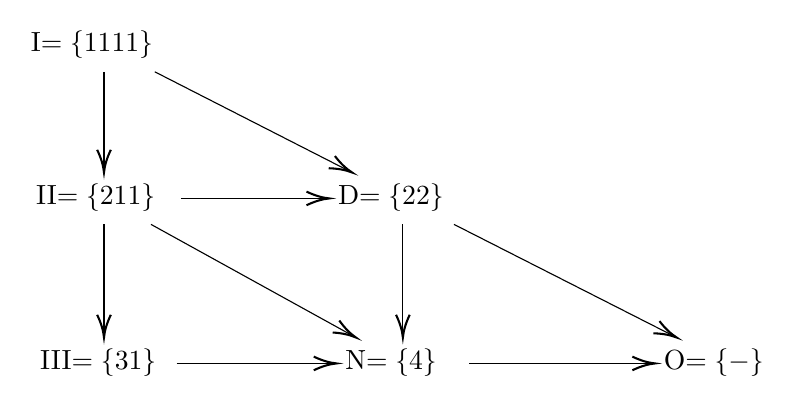
\begin{tikzpicture}[x=0.75pt,y=0.75pt,yscale=-1,xscale=1]
	%uncomment if require: \path (0,180); %set diagram left start at 0, and has height of 180
	
	
	
	% Text Node
	\draw (146,4) node [anchor=north west][inner sep=0.75pt]   [align=left] {I$=\{1111\}$};
	% Text Node
	\draw (148.5,77.5) node [anchor=north west][inner sep=0.75pt]   [align=left] {II$=\{211\}$};
	% Text Node
	\draw (294,77.5) node [anchor=north west][inner sep=0.75pt]   [align=left] {D$=\{22\}$};
	% Text Node
	\draw (150.5,157) node [anchor=north west][inner sep=0.75pt]   [align=left] {III$=\{31\}$};
	% Text Node
	\draw (297.5,157) node [anchor=north west][inner sep=0.75pt]   [align=left] {N$=\{4\}$};
	% Text Node
	\draw (451,157) node [anchor=north west][inner sep=0.75pt]   [align=left] {O$=\{-\}$};
	% Connection
	\draw    (182.5,25) -- (182.5,71.5) ;
	\draw [shift={(182.5,73.5)}, rotate = 270] [color={rgb, 255:red, 0; green, 0; blue, 0 }  ][line width=0.75]    (10.93,-3.29) .. controls (6.95,-1.4) and (3.31,-0.3) .. (0,0) .. controls (3.31,0.3) and (6.95,1.4) .. (10.93,3.29)   ;
	% Connection
	\draw    (206.99,25) -- (300.23,72.59) ;
	\draw [shift={(302.01,73.5)}, rotate = 207.04] [color={rgb, 255:red, 0; green, 0; blue, 0 }  ][line width=0.75]    (10.93,-3.29) .. controls (6.95,-1.4) and (3.31,-0.3) .. (0,0) .. controls (3.31,0.3) and (6.95,1.4) .. (10.93,3.29)   ;
	% Connection
	\draw    (219.5,86) -- (289,86) ;
	\draw [shift={(291,86)}, rotate = 180] [color={rgb, 255:red, 0; green, 0; blue, 0 }  ][line width=0.75]    (10.93,-3.29) .. controls (6.95,-1.4) and (3.31,-0.3) .. (0,0) .. controls (3.31,0.3) and (6.95,1.4) .. (10.93,3.29)   ;
	% Connection
	\draw    (182.5,98.5) -- (182.5,151) ;
	\draw [shift={(182.5,153)}, rotate = 270] [color={rgb, 255:red, 0; green, 0; blue, 0 }  ][line width=0.75]    (10.93,-3.29) .. controls (6.95,-1.4) and (3.31,-0.3) .. (0,0) .. controls (3.31,0.3) and (6.95,1.4) .. (10.93,3.29)   ;
	% Connection
	\draw    (217.5,165.5) -- (292.5,165.5) ;
	\draw [shift={(294.5,165.5)}, rotate = 180] [color={rgb, 255:red, 0; green, 0; blue, 0 }  ][line width=0.75]    (10.93,-3.29) .. controls (6.95,-1.4) and (3.31,-0.3) .. (0,0) .. controls (3.31,0.3) and (6.95,1.4) .. (10.93,3.29)   ;
	% Connection
	\draw    (205.14,98.5) -- (302.11,152.03) ;
	\draw [shift={(303.86,153)}, rotate = 208.9] [color={rgb, 255:red, 0; green, 0; blue, 0 }  ][line width=0.75]    (10.93,-3.29) .. controls (6.95,-1.4) and (3.31,-0.3) .. (0,0) .. controls (3.31,0.3) and (6.95,1.4) .. (10.93,3.29)   ;
	% Connection
	\draw    (326.5,98.5) -- (326.5,151) ;
	\draw [shift={(326.5,153)}, rotate = 270] [color={rgb, 255:red, 0; green, 0; blue, 0 }  ][line width=0.75]    (10.93,-3.29) .. controls (6.95,-1.4) and (3.31,-0.3) .. (0,0) .. controls (3.31,0.3) and (6.95,1.4) .. (10.93,3.29)   ;
	% Connection
	\draw    (351.11,98.5) -- (456.61,152.09) ;
	\draw [shift={(458.39,153)}, rotate = 206.93] [color={rgb, 255:red, 0; green, 0; blue, 0 }  ][line width=0.75]    (10.93,-3.29) .. controls (6.95,-1.4) and (3.31,-0.3) .. (0,0) .. controls (3.31,0.3) and (6.95,1.4) .. (10.93,3.29)   ;
	% Connection
	\draw    (358.5,165.5) -- (446,165.5) ;
	\draw [shift={(448,165.5)}, rotate = 180] [color={rgb, 255:red, 0; green, 0; blue, 0 }  ][line width=0.75]    (10.93,-3.29) .. controls (6.95,-1.4) and (3.31,-0.3) .. (0,0) .. controls (3.31,0.3) and (6.95,1.4) .. (10.93,3.29)   ;
	
\end{tikzpicture}
	\caption{根据主类光旋量方向的重合程度可以将外尔旋量分类成不同种类}
	\label{fig:Petrov}
\end{figure}

除此之外,根据外尔标量的定义,我们可以给出不同Petrov时空中,外尔标量为零的个数。如果我们选择$\xi ^{\boldsymbol{A}} =o^{\boldsymbol{A}}$,即$v^{\boldsymbol{a}} =l^{\boldsymbol{a}}$,那么
\begin{equation*}
	\upPsi _{\boldsymbol{ABCD}} o^{\boldsymbol{A}} o^{\boldsymbol{B}} o^{\boldsymbol{C}} o^{\boldsymbol{D}} =\upPsi _{0} ,
\end{equation*}
即如果时空为Petrov-I型,那么可以选择$\upPsi _{0} =0$。同样的,如果$l^{\boldsymbol{a}}$为Petrov-II型时空的主零方向,那么$\upPsi _{0} =\upPsi _{1} =0$。如果$l^{\boldsymbol{a}}$为Petrov-D型时空的第一个主零方向,且$n^{\boldsymbol{a}} =\iota ^{\boldsymbol{A}} \iota ^{\boldsymbol{A} '}$为第二个主零方向,那么除了$\upPsi _{0} =\upPsi _{1} =0$,我们还有$\upPsi _{4} =\upPsi _{3} =0$。同样的,III型和N型分别对应了$\upPsi _{0} =\upPsi _{1} =\upPsi _{2} =0$和$\upPsi _{0} =\upPsi _{1} =\upPsi _{2} =\upPsi _{3} =0$,而O型时空所有的外尔标量都为零,即共形平坦。


\subsection{哥德堡-萨赫定理}

现在我们考虑里奇张量为零,即黎曼张量与外尔张量重合的时空。这时我们有定理\parencite{chandrasekhar1998mathematical,goldberg2009republication}

\begin{them}[label={Goldberg-Sachs Theorem}]{哥德堡-萨赫定理(Goldberg-Sachs Theorem)}
	如果外尔张量是II型,且选择了$l^{\boldsymbol{a}}$作为主类光方向,即$\upPsi _{0} =\upPsi _{1} =0$,那么我们有
	\begin{equation*}
		\kappa =\sigma =0.
	\end{equation*}
	反之,如果$\kappa =\sigma =0$,那么
	\begin{equation*}
		\upPsi _{0} =\upPsi _{1} =0,
	\end{equation*}
	且外尔张量是II型。
\end{them}

\begin{proof}
	我们先来证明正命题。如果$\upPsi _{0} =\upPsi _{1} =0$,那么此时的比安基恒等式为
	\begin{equation*}
		\begin{cases}
			3\kappa \upPsi _{2} & =0\\
			D\upPsi _{2} & =-2\kappa \upPsi _{3} +3\rho \upPsi _{2}\\
			D\upPsi _{3} -\delta '\upPsi _{2} & =-\kappa \upPsi _{4} -2( \epsilon -\rho ) \upPsi _{3} +3\pi \upPsi _{2} ,
		\end{cases}
	\end{equation*}
	以及
	\begin{equation*}
		\begin{cases}
			3\sigma \upPsi _{2} & =0\\
			-\upDelta \upPsi _{2} & =2\sigma \upPsi _{3} -3\tau \upPsi _{2}\\
			D'\upPsi _{2} -\delta \upPsi _{3} & =-3\mu \upPsi _{2} -2( \tau -\beta ) \upPsi _{3} +\sigma \upPsi _{4} ,
		\end{cases}
	\end{equation*}
	由于时空不平坦,即$\upPsi _{2} ,\upPsi _{3} ,\upPsi _{4}$不全为零,那么$\kappa =\sigma =0$。
	
	
	
	现在来证明反论。由于标架有$6$个自由度,我们可以选择标架使得$\epsilon =0$,此时满足$\kappa =\sigma =0$,且包含这些量的里奇恒等式为
	\begin{equation}
		\begin{aligned}
			D\rho  & =\rho ^{2}\\
			\upPsi _{0} & =0\\
			D\tau  & =(\overline{\tau } +\pi )\rho +\upPsi _{1}
		\end{aligned}
		\label{eq:5.95}
	\end{equation}
	以及
	\begin{equation}
		\begin{aligned}
			D\beta  & =\overline{\rho } \beta +\upPsi _{1}\\
			\delta \rho  & =(\overline{\alpha } +\beta )\rho +(\rho -\overline{\rho } )\tau -\upPsi _{1} .
		\end{aligned}
		\label{eq:5.96}
	\end{equation}
	从\ref{eq:5.95}的第二个式子中我们给出$\upPsi _{0} =0$。此时,比安基恒等式为
	\begin{equation}
		\begin{aligned}
			D\upPsi _{1} & =4\rho \upPsi _{1}\\
			\delta \upPsi _{1} & =2(2\tau +\beta )\upPsi _{1} ,
		\end{aligned}
		\label{eq:5.97}
	\end{equation}
	以及$D,\delta $的对易子给出
	\begin{equation}
		D\delta -\delta D=(\overline{\pi } -\overline{\alpha } -\beta )D+\overline{\rho } \delta .
		\label{eq:5.98}
	\end{equation}
	现在,我们可以进一步选择规范使得$\tau =0$, 那么\ref{eq:5.97}给出
	\begin{equation*}
		\begin{cases}
			D\ln \upPsi _{1} & =4\rho ,\\
			\delta \ln \upPsi _{2} & =2\beta ,
		\end{cases}
	\end{equation*}
	故
	\begin{equation*}
		(D\delta -\delta D)\ln \upPsi _{1} =2D\beta -4\delta \rho .
	\end{equation*}
	现在,将上式的右侧带入\ref{eq:5.96}给出
	\begin{equation}
		(D\delta -\delta D)\ln \upPsi _{1} =2\overline{\rho } \beta -4(\overline{\alpha } +\beta )\rho +6\upPsi _{1} .
		\label{eq:5.99}
	\end{equation}
	然而,如果我们直接将对易子\ref{eq:5.98}应用在$\ln \upPsi _{1}$上,我们有
	\begin{equation}
		\begin{aligned}
			(D\delta -\delta D)\ln \upPsi _{1} & =(\overline{\pi } -\overline{\alpha } -\beta )D\ln \upPsi _{1} +\overline{\rho } \delta \ln \upPsi _{1}\\
			& =4(\overline{\pi } -\overline{\alpha } -\beta )\rho +2\beta \overline{\rho } .
		\end{aligned}
		\label{eq:5.100}
	\end{equation}
	为了保证\ref{eq:5.99}和\ref{eq:5.100}两侧相同,我们必须有
	\begin{equation*}
		\upPsi _{1} =\frac{2}{3}\overline{\pi } \rho ,
	\end{equation*}
	而\ref{eq:5.95}的第三式对于$\tau =0$有
	\begin{equation*}
		\upPsi _{1} =-\overline{\pi } \rho ,
	\end{equation*}
	这意味着我们必须有
	\begin{equation*}
		\upPsi _{1} =0.
	\end{equation*}
	至此正反两题证毕。
\end{proof}

哥德堡-萨赫定理的一个直接推论是,如果时空是Petrov-D型,那么当两个主类光方向$l^{\boldsymbol{a}} ,n^{\boldsymbol{a}}$重合时,即当且仅当
\begin{equation*}
	\upPsi _{0} =\upPsi _{1} =\upPsi _{3} =\upPsi _{4} =0
\end{equation*}
时,我们有
\begin{equation*}
	\kappa =\sigma =\nu =\lambda =0.
\end{equation*}
值得注意的是,广义相对论的黑洞解全部都是Petrov-D型的\parencite{chandrasekhar1998mathematical},因此我们总是能够令自旋系数$\kappa ,\sigma ,\lambda ,\nu $和除了$\upPsi _{2}$以外的外尔标量为零,这也是纽曼-彭罗斯形式对于它们特别有效的原因。